% !TeX spellcheck = eu_ES
\documentclass[eu]{ifirak}\usepackage[]{graphicx}\usepackage[]{color}
%% maxwidth is the original width if it is less than linewidth
%% otherwise use linewidth (to make sure the graphics do not exceed the margin)
\makeatletter
\def\maxwidth{ %
  \ifdim\Gin@nat@width>\linewidth
    \linewidth
  \else
    \Gin@nat@width
  \fi
}
\makeatother

\definecolor{fgcolor}{rgb}{0, 0, 0}
\newcommand{\hlnum}[1]{\textcolor[rgb]{0.659,0.4,0.051}{#1}}%
\newcommand{\hlstr}[1]{\textcolor[rgb]{0.659,0.4,0.051}{#1}}%
\newcommand{\hlcom}[1]{\textcolor[rgb]{0.333,0.533,0.09}{#1}}%
\newcommand{\hlopt}[1]{\textcolor[rgb]{0,0,0}{#1}}%
\newcommand{\hlstd}[1]{\textcolor[rgb]{0,0,0}{#1}}%
\newcommand{\hlkwa}[1]{\textcolor[rgb]{0.133,0.224,0.659}{\textbf{#1}}}%
\newcommand{\hlkwb}[1]{\textcolor[rgb]{0.549,0.114,0.412}{\textbf{#1}}}%
\newcommand{\hlkwc}[1]{\textcolor[rgb]{0.659,0.573,0.133}{\textbf{#1}}}%
\newcommand{\hlkwd}[1]{\textcolor[rgb]{0.659,0.133,0.482}{#1}}%

\usepackage{framed}
\makeatletter
\newenvironment{kframe}{%
 \def\at@end@of@kframe{}%
 \ifinner\ifhmode%
  \def\at@end@of@kframe{\end{minipage}}%
  \begin{minipage}{\columnwidth}%
 \fi\fi%
 \def\FrameCommand##1{\hskip\@totalleftmargin \hskip-\fboxsep
 \colorbox{shadecolor}{##1}\hskip-\fboxsep
     % There is no \\@totalrightmargin, so:
     \hskip-\linewidth \hskip-\@totalleftmargin \hskip\columnwidth}%
 \MakeFramed {\advance\hsize-\width
   \@totalleftmargin\z@ \linewidth\hsize
   \@setminipage}}%
 {\par\unskip\endMakeFramed%
 \at@end@of@kframe}
\makeatother

\definecolor{shadecolor}{rgb}{.97, .97, .97}
\definecolor{messagecolor}{rgb}{0, 0, 0}
\definecolor{warningcolor}{rgb}{1, 0, 1}
\definecolor{errorcolor}{rgb}{1, 0, 0}
\newenvironment{knitrout}{}{} % an empty environment to be redefined in TeX

\usepackage{alltt}

\usepackage{amsmath,latexsym,amssymb,natbib}
\usepackage{listings}
\usepackage{ifcommands,subfigure}
\usepackage[T1]{fontenc}
\usepackage{tcolorbox}

\newcommand{\zkk}{\guillemotleft}
\newcommand{\skk}{\guillemotright}
\newcommand{\code}[1]{\texttt{#1}}
\newcommand{\eng}[1]{\textit{#1}}
\newcommand{\hgl}[1]{\zkk #1\skk\ }
\IfFileExists{upquote.sty}{\usepackage{upquote}}{}
\begin{document}
%\SweaveOpts{concordance=TRUE}
\ikasturtea{2014/2015}
\irakasgaia{Bilaketa Heuristikoak}
\title{BHLN: Populazioan oinarritutako algoritmoak}
\date{}
\irakaslea{Borja Calvo, Usue Mori}
\author{Borja Calvo, Usue Mori}


\tel{943 01 50 13}
\mail{borja.calvo@ehu.es}




\maketitle

\begin{abstract}
Aurreko kapituluan soluzio bakarrean oinarritzen diren zenbait algoritmo ikusi ditugu. Algoritmo hauek oso portaera ezberdina izan arren, badute ezaugarri komun bat: bilaketa prozesua soluzio batetik bestera mugitzen da, soluzioak banan-banan aztertuz. Ezaugarri hau dela eta, algoritmo hauek oso algoritmo egokiak dira bilaketa espazioaren eskualde interesgarriak arakatzeko --bilaketa areagotzeko, alegia--. Alabaina, hainbat kasutan emaitza onak lortzeko bilaketa dibertsifikatzea ere beharrezkoa da. Hau honela izanik, bilaketa lokalean oinarritzen diren algoritmo batzuk dibertsifikatzeko zenbait estrategia darabilte, adibide nabarmenena tabu bilaketaren epe-luzeko memoria izanik.

Kapitulu honetan soluzioen banan-banakako azterketa alde batera utzita, soluzio multzoak erabiltzeari ekingo diogu, horixe baita, hain justu, populazioetan oinarritzen diren algoritmoen filosofia. Algoritmoaren pausu bakoitzean, soluzio bakar bat izan beharrean, soluzio multzo bat izango dugu. Testuinguru batzuetan soluzio multzo honi \hgl{soluzio-populazioa} deritzo eta, hortik, algoritmo hauen izena. Algoritmo hauekin, bilaketa prozesuan zehar, soluzio multzo hori aldatuz joango da helburu funtzioaren gidaritzapean, gelditze irizpide bat bete arte.

Oro har, populazioan oinarritutako algoritmoak bi multzotan banatu ditzakegu: algoritmo ebolutiboak eta \eng{swarm intelligence}-an oinarritutakoak. Lehenengo kategoriako algoritmoek, populazioa eboluzionarazten dute, teknika ezberdinak erabiliz, honek geroz eta soluzio hobeak izan ditzan. Adibiderik ezagunenak algoritmo genetikoak dira. Bigarren motako algoritmoak, berriz, zenbait animalien portaeran oinarritzen dira. Hauen arteko adibiderik ezagunenak, esate baterako, inurriek, janaria eta inurritegiaren arteko distantziarik motzena topatzeko darabilten mekanismoa imitatzen du.

Kapitulua bi zatitan banaturik dago, bakoitza populazioan oinarritutako algoritmo mota bati eskeinita. Lehenengo zatian, algoritmo ebolutiboen eskema orokorra ikusi ondoren, algoritmo genetikoak \cite{holland1975} eta EDAk \cite{larranaga2002,lozano2006} aurkeztuko dira. Bigarren zatian ordea, \eng{swarm intelligence} \cite{blum2008} arloan proposaturiko bi algoritmo aztertuko dira.
\end{abstract}


\section{Algoritmo Ebolutiboak}\label{sec:ebolutiboak}
1859. urtean Charles R. Darwinek \eng{On the Origin of the Species by Means of Natural Selection, or the Preservation of Favoured Races in the Struggle for Life} liburua argitaratu zuen. Tituluak berak adierazten duen bezala, liburu honetan Darwinek hautespen naturalaren teoria aurkeztu zuen. 

Eboluzioaren teoriak dioenez, belaunalditik belaunaldira zenbait mekanismoen bidez --mutazioak, esate baterako-- aldaketak ematen dira espezieetan. Aldaketa hauetako batzuei esker indibiduoak hobeto egokitzen dira haien ingurunera eta, ondorioz, bizirik mantentzeko eta, batez ere, ugaltzeko probabilitateak handitzen dira. Era berean, noski, aldaketa batzuk kaltegarriak izan daitezke, bizitzeko aukerak murriztuz. Kontutan hartuz aipatutako aldaketak heredatu egiten direla, ezaugarri onak generazioz generazio mantentzen dira; kaltegarriak direnek, ostera, galtzeko joera izaten dute. Prozesu honen bidez, espezieak haien ingurunera geroz eta hobeto egokitzeko gai dira.

Hirurogeigarren hamarkadan ikertzaileek Darwinen lana inspiraziotzat hartu zuten optimizazio metahuristikoak diseinatzeko eta geroztik, konputazio ebolutiboa konputazio zientzien arlo bereizia bilakatu da. Atal honetan bi algoritmo mota aztertuko ditugu, algoritmo genetiko klasikoak \cite{holland1975} eta EDAk (\eng{Estimation of Distribution Algorithms}) \cite{larranaga2002, lozano2006}.


\begin{figure}[t]
\centering
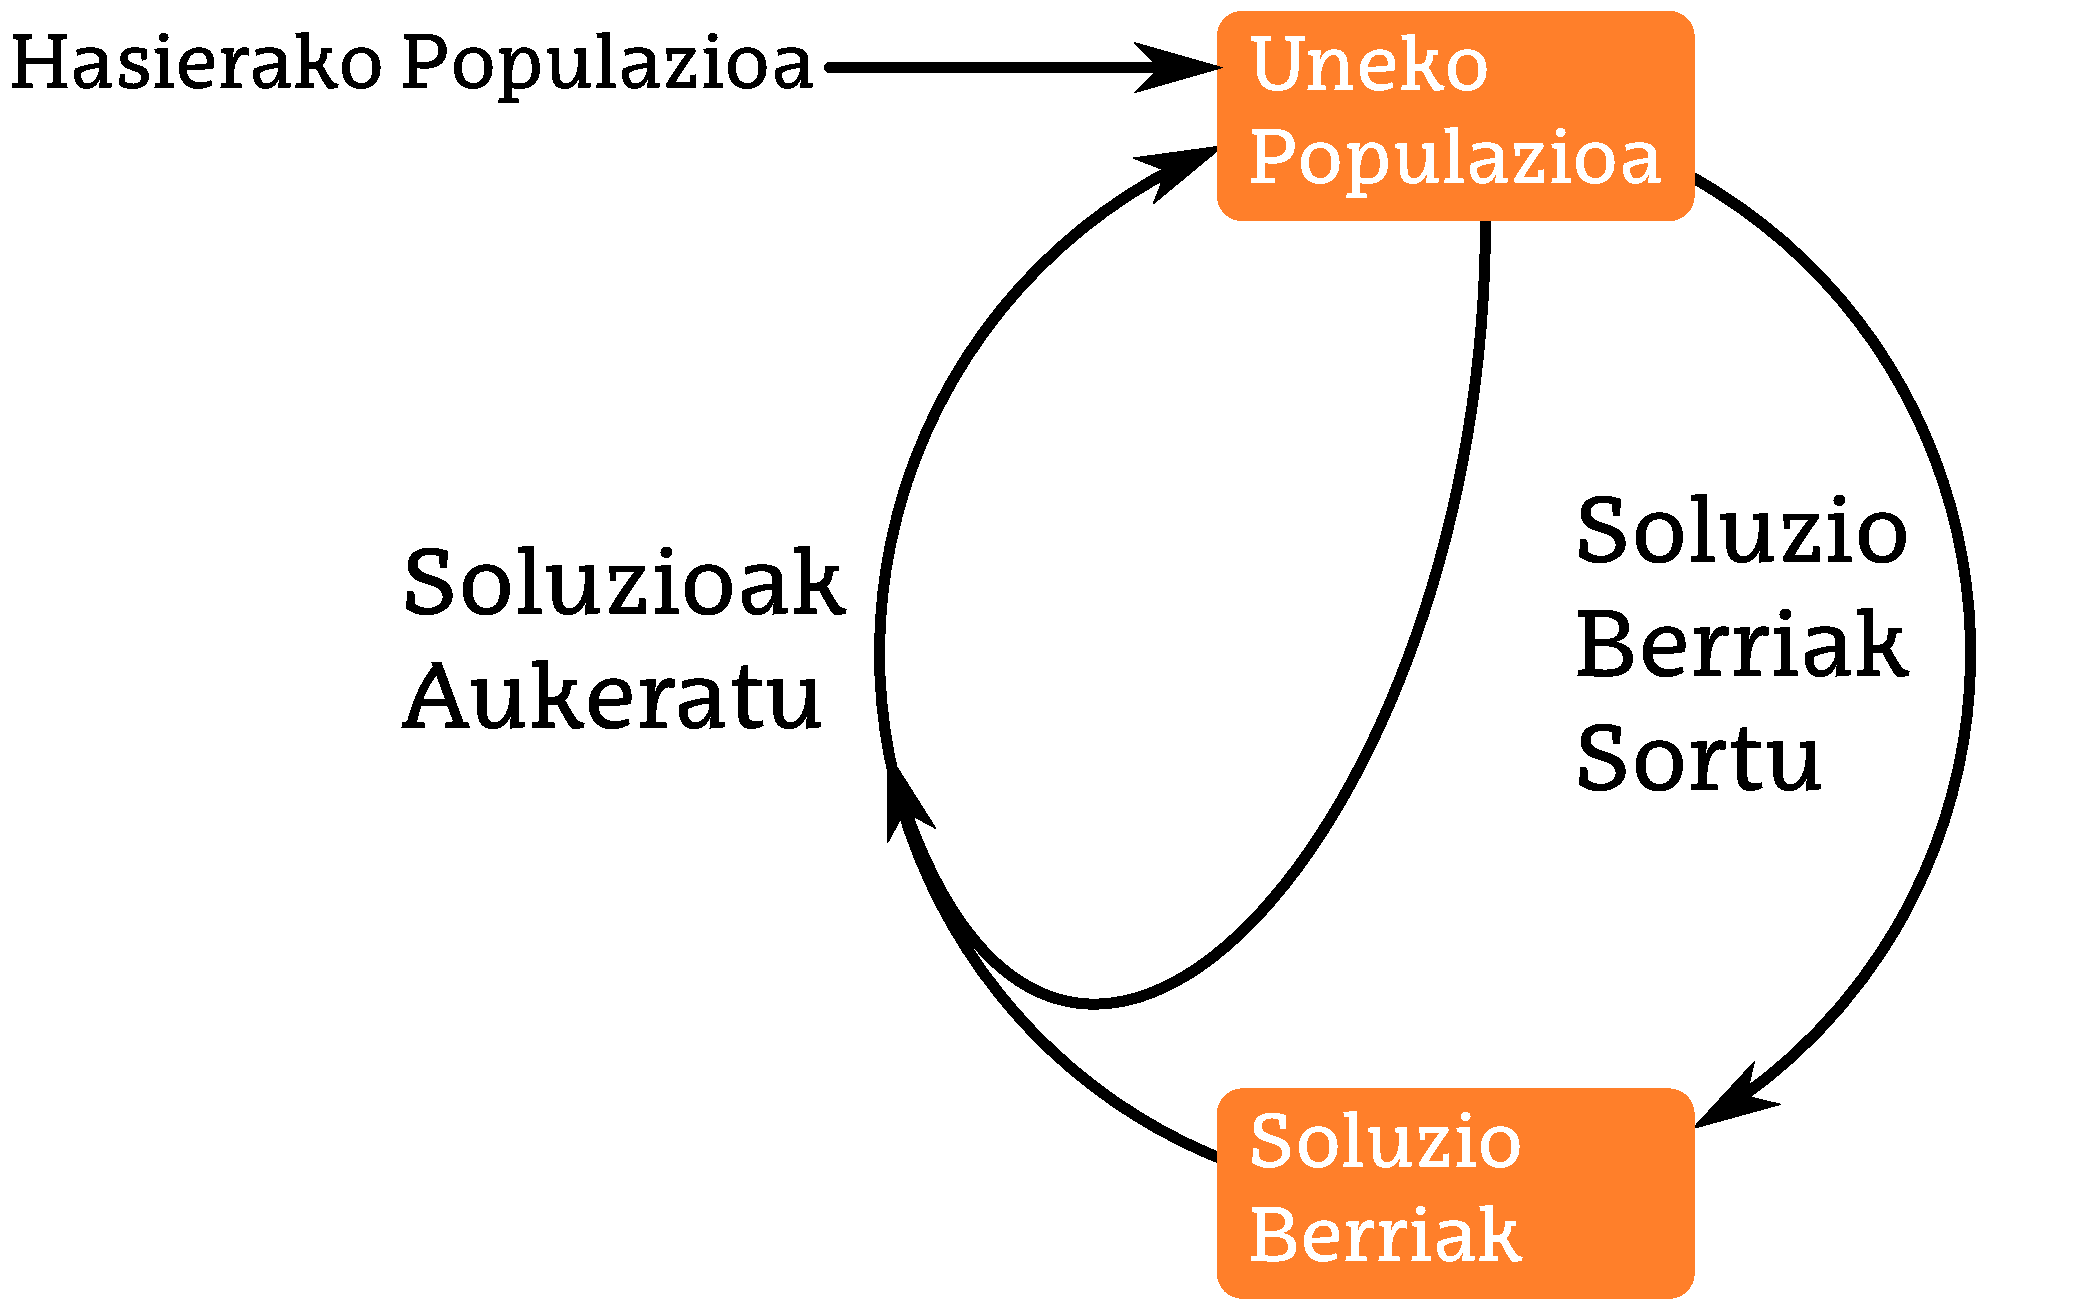
\includegraphics[height=0.2\textheight]{./Irudiak/AEB}
\caption{Algoritmo ebolutiboen eskema orokorra}
\label{fig:alg.evol}
\end{figure}


Diferentziak diferentzia, algoritmo ebolutibo guztiek \ref{fig:alg.evol} irudiko eskema orokorra jarraitzen dute. Eskema orokor honetan, bi dira giltzarri diren elementuak: soluzio berrien sorkuntza eta soluzioen hautespena. Algoritmoaren sarrera-puntua hasierako populazioa izango da; populazio horretatik abiatuz, algoritmoa begizta nagusian sartzen da, non bi pausu txandakatzen diren. Lehenik, uneko populazioko soluzioetatik abiatuz, soluzio berri multzo bat sortuko da. Ondoren, soluzio berri hauek eta uneko populazioko soluzioak kontutan hartuz, naturan bezala, hurrengo belaunaldiara pasatzeko soluzio onak aukeratuko ditugu, eta populazio berri bat sortuko dugu. Begizta nagusia etengabekoa denez, zenbait irizpide ezberdin proposatu dira algoritmoa amaitutzat emateko.

Hurrengo atalean, algoritmo orokor honen urratsak sakonago aztertuko ditugu. Hasteko, algoritmo ebolutibo guztietan antzerakoak diren pausuak azalduko ditugu eta ondoren, bi algoritmo ezberdinen xehetasunetan jarriko dugu arreta. 

\subsection{Urrats orokorrak}

Ondorengo ataletan ikusiko ditugun algoritmoen arteko diferentzia nagusia soluzio berrien sorkuntzan datza. Gaionontzeko urratsak era antzekoan burutzen dira algoritmo ezberdinetan eta horiei buruz hitz egingo dugu atal honetan.

\subsubsection{Populazioaren hasieraketa}

Nahiz eta askotan garrantzi gutxi eman, hasierako populazioa da algoritmoaren abia-puntua eta, hortaz, bere sorkuntza oso pausu garrantzitsua da, eragin handia izaten duelako algoritmoak lortutako azken emaitzan. 

Algoritmoen xedea soluzio onak topatzea izanda, pentsa dezakegu hasierako populazio on bat soluzio onez osatuta egon behar dela; alabaina, dibertsitatea soluzioen kalitatea bezain garrantzitsua da. Nahiz eta onak izan, populazioa oso soluzio antzerakoez osatuta badago, populazioaren eboluzioa oso zaila izango da eta algoritmoak azkarregi konbergitu dezake optimoa ez den soluzio batera. 

Hortaz, hasierako populazioa sortzean bi aspektu izan behar ditugu kontutan: kalitatea eta dibertsitatea. Kasu gehienetan ausazko hasieraketa erabiltzen da lehen populazioa sortzeko, hau da, ausazko soluzioak sortzen dira populazioa osatu arte. Estrategia hau erabiliz dibertsitate handiko populazioa sortuko dugu, baina kalitatea ez da handia izango. 

Ausazko laginketak lortutakoa baina dibertsitate handiagoa bermatu nahi badugu, --sasiausazko-- prozedura batzuk erabil ditzakegu. Hori dela eta, proposatu dira beste prozedura batzuk populazioak sasi-ausaz sortzeko dibertsitatea maximizatuz. Esate baterako, dibertsifikazio sekuentziala aplikatu dezakegu, zeinak soluzio berri bat onartzen duen soilik populazioan dauden soluzioekiko distantzia minimo batera badago. Adibide moduan, demagun 25 tamainako bektore bitarren 10 tamainako populazio bat sortu nahi dugula. Dibertsitatea bermatzeko populazioko soluzioen arteko Hamming distantzia minimoak 10-ekoa izan behar duela inposa dezakegu. 

Jarraian dagoen kodeak horrelako populazioak sortzen ditu. Lehenik, Hamming distantzia neurtzeko eta ausazko bektore bitarrak sortzeko funtzioak sortzen ditugu:

\begin{knitrout}
\definecolor{shadecolor}{rgb}{1, 1, 1}\color{fgcolor}\begin{kframe}
\begin{alltt}
\hlstd{> }\hlstd{hammDistance} \hlkwb{<-} \hlkwa{function} \hlstd{(}\hlkwc{v1}\hlstd{,} \hlkwc{v2}\hlstd{) \{}
\hlstd{+ }  \hlstd{d} \hlkwb{<-} \hlkwd{sum}\hlstd{(v1} \hlopt{!=} \hlstd{v2)}
\hlstd{+ }  \hlkwd{return}\hlstd{(d)}
\hlstd{+ }\hlstd{\}}
\hlstd{> }
\hlstd{> }\hlstd{createRndBinary} \hlkwb{<-} \hlkwa{function}\hlstd{(}\hlkwc{n}\hlstd{) \{}
\hlstd{+ }  \hlkwd{return} \hlstd{(}\hlkwd{runif}\hlstd{(n)} \hlopt{>} \hlnum{0.5}\hlstd{)}
\hlstd{+ }\hlstd{\}}
\end{alltt}
\end{kframe}
\end{knitrout}

 Gero, soluzioak ausaz sortzen ditugu eta, distantzia minimoko baldintza bete ezean, deusestatu egiten ditugu; prozedura nahi ditugun soluzio kopurua lortu arte exekutatzen da. 

\begin{knitrout}
\definecolor{shadecolor}{rgb}{1, 1, 1}\color{fgcolor}\begin{kframe}
\begin{alltt}
\hlstd{> }\hlstd{sol.size} \hlkwb{<-} \hlnum{25}
\hlstd{> }\hlstd{pop.size} \hlkwb{<-} \hlnum{10}
\hlstd{> }\hlstd{min.distance} \hlkwb{<-} \hlnum{10}
\hlstd{> }\hlstd{population} \hlkwb{<-} \hlkwd{list}\hlstd{(}\hlkwd{createRndBinary}\hlstd{(sol.size))}
\hlstd{> }\hlkwa{while} \hlstd{(}\hlkwd{length}\hlstd{(population)} \hlopt{<} \hlstd{pop.size) \{}
\hlstd{+ }  \hlstd{new.sol} \hlkwb{<-} \hlkwd{createRndBinary}\hlstd{(sol.size)}
\hlstd{+ }  \hlstd{distances} \hlkwb{<-} \hlkwd{lapply}\hlstd{(population,}
\hlstd{+ }                      \hlkwc{FUN}\hlstd{=}\hlkwa{function}\hlstd{(}\hlkwc{x}\hlstd{) \{}
\hlstd{+ }                        \hlkwd{return}\hlstd{(}\hlkwd{hammDistance} \hlstd{(x, new.sol))}
\hlstd{+ }                      \hlstd{\})}
\hlstd{+ }  \hlkwa{if} \hlstd{(}\hlkwd{min}\hlstd{(}\hlkwd{unlist}\hlstd{(distances))} \hlopt{<=} \hlstd{min.distance) \{}
\hlstd{+ }    \hlstd{population[[}\hlkwd{length}\hlstd{(population)} \hlopt{+} \hlnum{1}\hlstd{]]} \hlkwb{<-} \hlstd{new.sol}
\hlstd{+ }  \hlstd{\}}
\hlstd{+ }\hlstd{\}}
\end{alltt}
\end{kframe}
\end{knitrout}


Prozedura hau ez da batere eraginkorra, zenbait kasutan soluzio asko aztertu beharko baititugu populazioa osatu arte. Hala, beste alternatiba eraginkorrago bat dibertsifikazio paraleloa da. Kasu honetan bilaketa espazioa zatitu egiten da eta azpi-espazio bakoitzetik ausazko soluzio bat erauzten da.

Orain arte dibertsitateari bakarrik erreparatu diogu. Aldiz, hasierako popuazioaren kalitatea hobetu nahi izanez gero, hasieraketa heuristikoak erabil daitezke. Hau lortzeko era sinple bat, GRASP algoritmoetan ausazko soluzioak sortzeko erabiltzen diren prozedurak erabiltzea da. Ondoko lerroetan Bavierako hirien TSP problemarako adibide bat ikus dezakegu. Lehenik, problema kargatuko dugu.

\begin{knitrout}
\definecolor{shadecolor}{rgb}{1, 1, 1}\color{fgcolor}\begin{kframe}
\begin{alltt}
\hlstd{> }\hlstd{url} \hlkwb{<-} \hlkwd{system.file}\hlstd{(}\hlstr{"bays29.xml.zip"}\hlstd{,} \hlkwc{package}\hlstd{=}\hlstr{"metaheuR"}\hlstd{)}
\hlstd{> }\hlstd{cost.matrix} \hlkwb{<-} \hlkwd{tsplibParser}\hlstd{(url)}
\end{alltt}
\end{kframe}
\end{knitrout}

Orain, \code{tspGreedy} funtzioan oinarrituta, ausazko soluzio onak sortzeko funtzio bat definitzen dugu.

\begin{knitrout}
\definecolor{shadecolor}{rgb}{1, 1, 1}\color{fgcolor}\begin{kframe}
\begin{alltt}
\hlstd{> }\hlstd{createRndSolution} \hlkwb{<-} \hlkwa{function}\hlstd{(}\hlkwc{cl.size}\hlstd{=}\hlnum{5}\hlstd{) \{}
\hlstd{+ }  \hlkwd{tspGreedy}\hlstd{(}\hlkwc{cmatrix}\hlstd{=cost.matrix,} \hlkwc{cl.size}\hlstd{=cl.size)}
\hlstd{+ }\hlstd{\}}
\end{alltt}
\end{kframe}
\end{knitrout}

Aurreko kapituluetan azaldu bezala, \code{tspGreedy} funtzioak TSP-rako algoritmo eraikitzaile bat inplementatzen du; pausu bakoitzean, uneko hiritik zein hirira mugituko garen erabakitzen da, gertuen dauden \code{cl.size} hirietatik --5, gure kasuan-- bat ausaz aukeratuz. Honetan oinarrituz, populazioa sortzeko funtzio hau erabiliko dugu.

\begin{knitrout}
\definecolor{shadecolor}{rgb}{1, 1, 1}\color{fgcolor}\begin{kframe}
\begin{alltt}
\hlstd{> }\hlstd{pop.size} \hlkwb{<-} \hlnum{25}
\hlstd{> }\hlstd{population} \hlkwb{<-} \hlkwd{lapply}\hlstd{(}\hlnum{1}\hlopt{:}\hlstd{pop.size,}
\hlstd{+ }                     \hlkwc{FUN}\hlstd{=}\hlkwa{function}\hlstd{(}\hlkwc{x}\hlstd{) \{}
\hlstd{+ }                       \hlkwd{return}\hlstd{(}\hlkwd{createRndSolution}\hlstd{())}
\hlstd{+ }                     \hlstd{\})}
\end{alltt}
\end{kframe}
\end{knitrout}

Hautagaien zerrendaren tamainari (\code{cl.size}) problemaren tamainaren balioa ezartzen badiogu, pausu bakoitzean, aukera guztietatik bat ausaz hartuko dugu, hots, guztiz ausazkoak diren soluzioak sortuko ditugu. Azken aukera honekin, populazioaren kalitatea goiko kodearekin lortutakoa baino okerragoa izango da:

\begin{knitrout}
\definecolor{shadecolor}{rgb}{1, 1, 1}\color{fgcolor}\begin{kframe}
\begin{alltt}
\hlstd{> }\hlstd{rnd.population} \hlkwb{<-} \hlkwd{lapply} \hlstd{(}\hlnum{1}\hlopt{:}\hlstd{pop.size,}
\hlstd{+ }                          \hlkwc{FUN}\hlstd{=}\hlkwa{function}\hlstd{(}\hlkwc{x}\hlstd{) \{}
\hlstd{+ }                            \hlkwd{return}\hlstd{(}\hlkwd{createRndSolution}\hlstd{(}\hlkwc{cl.size}\hlstd{=}\hlkwd{ncol}\hlstd{(cost.matrix)))}
\hlstd{+ }                          \hlstd{\})}
\hlstd{> }\hlstd{tsp} \hlkwb{<-} \hlkwd{tspProblem}\hlstd{(cost.matrix)}
\hlstd{> }\hlstd{eval.heur} \hlkwb{<-} \hlkwd{unlist}\hlstd{(}\hlkwd{lapply}\hlstd{(population,} \hlkwc{FUN}\hlstd{=tsp}\hlopt{$}\hlstd{evaluate))}
\hlstd{> }\hlstd{eval.rnd} \hlkwb{<-} \hlkwd{unlist}\hlstd{(}\hlkwd{lapply}\hlstd{(rnd.population,} \hlkwc{FUN}\hlstd{=tsp}\hlopt{$}\hlstd{evaluate))}
\end{alltt}
\end{kframe}
\end{knitrout}


Bi populazioen ebaluazioak \eng{boxplot} baten bidez aldera ditzakegu:

\begin{knitrout}
\definecolor{shadecolor}{rgb}{1, 1, 1}\color{fgcolor}\begin{kframe}
\begin{alltt}
\hlstd{> }\hlstd{df} \hlkwb{<-} \hlkwd{rbind}\hlstd{(}\hlkwd{data.frame}\hlstd{(}\hlkwc{Method}\hlstd{=}\hlstr{"Heuristic"}\hlstd{,} \hlkwc{Evaluation}\hlstd{=eval.heur),}
\hlstd{+ }            \hlkwd{data.frame}\hlstd{(}\hlkwc{Method}\hlstd{=}\hlstr{"Random"}\hlstd{,} \hlkwc{Evaluation}\hlstd{=eval.rnd))}
\hlstd{> }\hlkwd{ggplot}\hlstd{(df,} \hlkwd{aes}\hlstd{(}\hlkwc{x}\hlstd{=Method,} \hlkwc{y}\hlstd{=Evaluation))} \hlopt{+} \hlkwd{geom_boxplot}\hlstd{()}
\end{alltt}
\end{kframe}
\end{knitrout}

\begin{figure}[t]
\centering
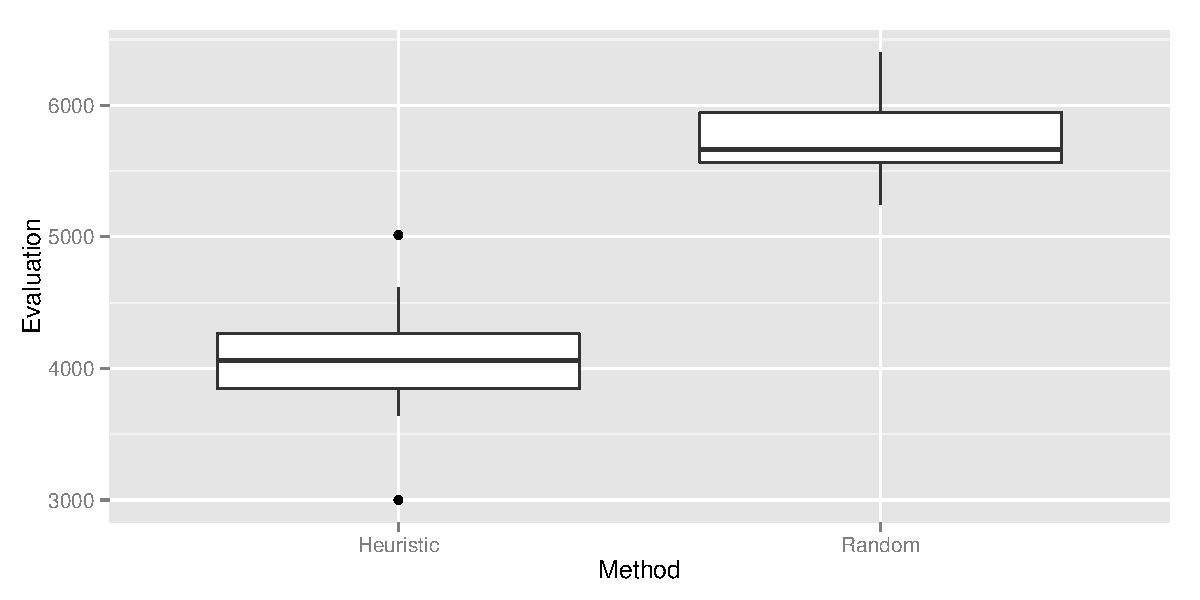
\includegraphics[height=0.33\textheight]{./Irudiak/plot_heur_vs_rnd-1}
\caption{Ausazko hasieraketa eta hasieraketa heuristikoaren arteko konparaketa. Y ardatzak metodo bakoitzarekin sortutako soluzioen \eng{fitness}-a adierazten du.}\label{fig:heur_vs_rnd_init_pop}
\end{figure}

\ref{fig:heur_vs_rnd_init_pop} irudiak lortutako emaitzak erakusten ditu. Helburua minimizazioa dela kontutan hartuz, argi eta garbi ikus daiteke heuristikoa erabiliz sortutako soluzioak hobeak direla.

Soluzioak sortzeko metodoak ez ezik, populazioaren tamainak ere badu eragin handia azken emaitzan, eta  egokitu beharreko oso parametro garrantzitsua da. Algoritmoak darabiltzan populazioak txikiegiak badira, dibertsitatea mantentzea oso zaila izango da eta, hortaz, belaunaldi gutxitan algoritmoak konbergitu egingo du, ziurrenik optimoa ez den soluzio batera. Beste aldetik, populazioak handiegiak badira, konbergentzia abiadura motelagoa izango da baina, ondorioz, kostu konputazionala ere handiagoa bilakatuko da; hurrengo atalean adibide baten bidez ikusiko dugu hau. Honenbestez, ez dago irizpide finkorik populazioen tamaina ezartzeko eta problema bakoitzerako balio egoki bat bilatu beharko da. Edonola ere, irizpide orokor gisa esan dezakegu populazioak azkar konbergitzen badu --hots, soluzioen arteko distantzia azkar txikitzen bada--, soluzio hobeak lortzeko modua populazioaren tamaina handitzea izan daitekeela. 


\subsubsection{Hautespena}

Algoritmo ebolutibotan populazioko soluzio batzuen aukeraketa urrats garrantzitsua da, populazioaren eboluzioa kontrolatzen duen prozesua baita. Orokorrean, populazioan dauden soluziorik onenak hautatzea da gehien erabiltzen den hautespen irizpidea: hautespen \zkk elitista\skk\. Alabaina, soluzio onak aukeratzea garrantzitsua bada ere, dibertsitatea mantentzearren, tarteka soluzio txarrak sartzea ere komenigarria izaten da. Hau zuzenean egin daiteke, baina badaude aukeraketa metodo egokiago batzuk soluzio txarrak estrategia probabilistikoak erabiliz aukeratzen dituztenak.

Erruleta-hautespena,  (\textit{Roulette Wheel selection}, ingelesez) deritzon estrategian soluzioak erruleta batean kokatzen dira; soluzio bakoitzari, bere ebaluazioarekiko proportzionala den, erruletaren zati bat esleituko zaio. Hau honela, \ref{fig:roulette} irudian ikus daitekeen bezala, erruleta jaurtitzen den bakoitzean indibiduo bat hautatzen da. Hautatua izateko probabilitatea erruleta zatiaren tamaina eta, hortaz, indibiduoen ebaluazioarekiko proportzionala da. Indibiduo bat baino gehiago aukeratu behar baldin badugu, behar adina erruleta jaurtiketa egin ditzakegu. 

Azkenik, esan beharra dago, \eng{fitness}aren magnitudea problema eta, batez ere, instantzien araberakoa dela. Hori dela eta, erruleta banatzeko probabilitateak zuzenean helburu funtzioaren balioak erabiliz kalkulatzen badira, oso distribuzio erradikalak izan ditzakegu. Arazo hau ekiditeko, helburu funtzioaren balioa zuzenean erabili beharrean soluzioen ranking-a erabiltzea posible da.

\begin{figure}[t]
\centering
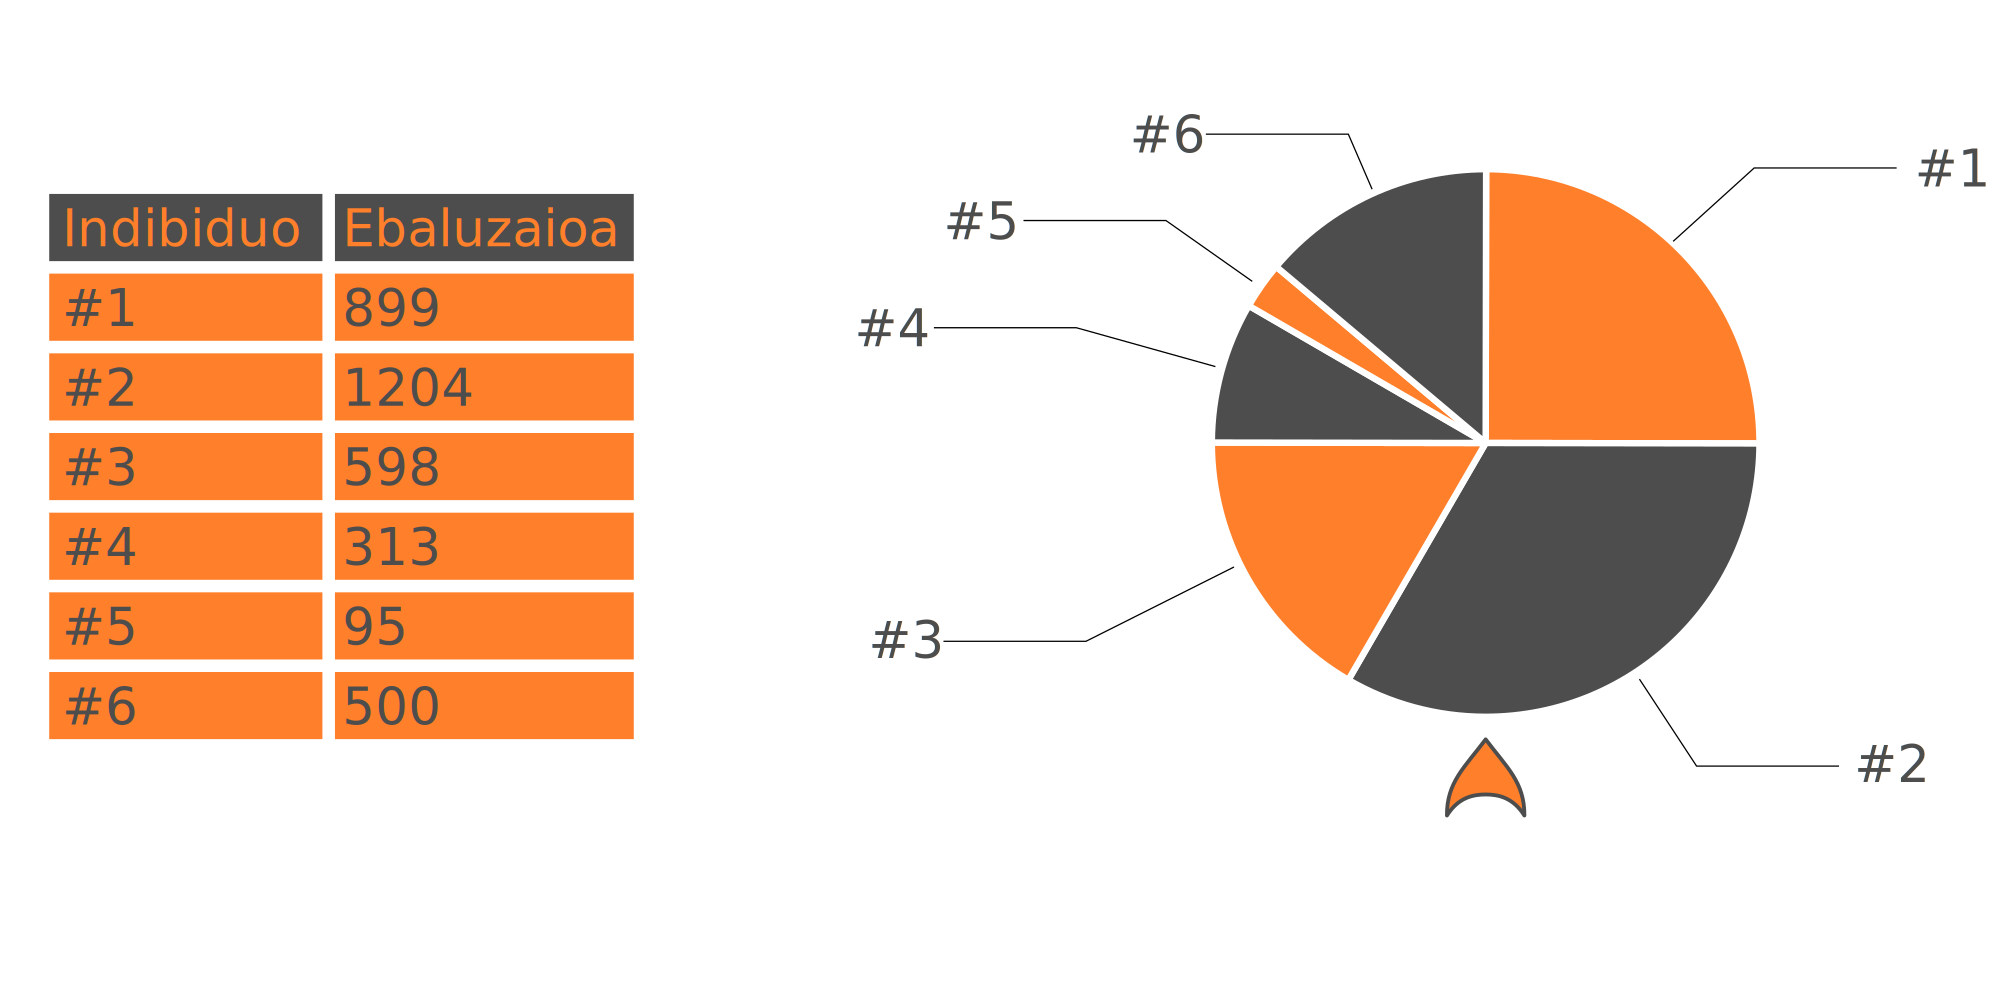
\includegraphics[width=0.7\linewidth]{./Irudiak/roulette}
\caption{Erruleta-hautespena. Indibiduo bakoitzaren erruletaren zatia bere ebaluazioarekiko proportzionala da. Erruleta jaurtitzen den bakoitzean indibiduo bat aukeratzen da, bere \eng{fitness}arekiko proportzionala den probabilitatearekin. Adibidean, 2. indibiduoa da hautatu dena.}
\label{fig:roulette}
\end{figure}

Beste hautespen probabilistiko mota bat Lehiaketa-hautespena da. Estrategia honekin soluzioen aukeraketa bi pausutan egiten da. Lehenengo urratsean indibiduo guztietatik azpi-multzo bat aukeratzen da, guztiz ausaz (ebaluazioa kontutan hartu barik). Ondoren, azpi-multzo honetatik soluziorik onena hautatzen dugu. Azpi-multzoen eraketa guztiz ausaz egiten denez, hauetako batzuk, oso soluzio txarrez osatuta egon daitezke. Kasu hauetan, nahiz eta onena aukeratu, populazio berrirako gordeko dugun soluzioa ez da ona izango eta, honenbestez, soluzio on eta txarren aukeraketa baimentzen du hautespen metodo honek. 

\subsubsection{Gelditze Irizpideak}

Lehen apiatu bezala, algoritmo ebolutiboen begizta nagusia amaigabea da eta, beraz, gelditzeko irizpideren bat ezarri behar dugu, bilaketak amaiera izan dezan. Hurbilketarik sinpleena irizpide estatikoak erabiltzea da, hala nola, denbora maximoa ezartzea, ebaluazioak mugatzea, etab.

Bestalde, gelditzeko irizpide dinamikoak, hau da, eboluzioaren prozesuari erreparatzen diotenak ere erabili daitezke. Balunaldiz belaunaldi populazioan dauden soluzioak geroz eta hobeak dira eta, aldi berean, populazioaren dibertsitatea murrizten da, soluzio batera konbergitzeko joerarekin. Hau hala izanik, populazioaren dibertsitatea gelditze irizpide dinamikoak eraikitzeko erabil daiteke.

Dibertsitatea soluzioei zein beraien \eng{fitness}-ari erreparatuz neur daiteke. Esate baterako, soluzioen arteko distatzia neurtzerik badago, indibiduoen arteko bataz besteko distantzia minimo bat ezar dezakegu gelditze irizpide gisa.

\subsubsection{Algoritmo Genetikoak}

Atal honetan algoritmo genetikoetan \cite{holland1975} soluzio berriak nola sortzen diren ikusiko dugu. Algoritmo genetikoak naturan espezieen eboluzioarekin gertatzen dena imitatzen dute eta, beraz, fenomeno honekin zenbait paralelismo ezar daitezke:

\begin{itemize}
\item Espezie bateko indibiduoak = Problemaren soluzioak
\item Indibiduoen egokitasuna --\eng{fitness}-a, alegia-- = Soluzioaren ebaluazioa
\item Espeziearen populazioa = Soluzio multzoa/populazioa
\item Ugalketa = Soluzio berrien sorkuntza
\end{itemize}

Beraz, algoritmo genetikoetan soluzio berriak sortzeko estrategiak diseinatzean indibiduen ugalketa prozesuan oinarrituko gara.  Ugalketa prozesuaren xedea zenbait indibiduo emanda --bi, normalean--, indibiduo berriak sortzea da. Ohikoena prozesu hau bi pausutan banatzea da: soluzioen gurutzaketa eta mutazioa. Lehenaren helburua \hgl{guraso}-soluzioek dituzten ezaugarriak soluzio berriei pasatzea da, espezieen gurutzaketan jazotzen den bezala. Bigarrenarena, berriz, sortutako soluzio berriei ezaugarri berriak eranstea da. Jarraian soluzioak maneiatzeko bi operadore hauek aztertuko ditugu.

\begin{figure}[tb]
\centering
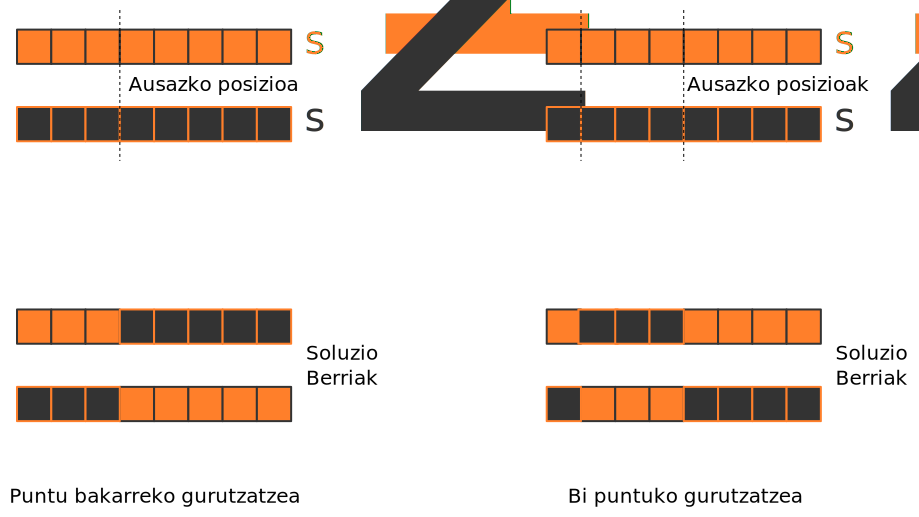
\includegraphics[width=0.7\linewidth]{./Irudiak/point_crossover}
\caption{Gurutzatze-operadoreak bektoreen bidezko kodeketarekin erabiltzeko}
\label{fig:point_crossover}
\end{figure}

\subsubsection{Gurutzaketa} 

Bi soluzio --edo gehiago-- gurutzatzen ditugunean euren propietateak sortutako soluzio berriei transmititzea da helburua. Optimizazio arloan, soluzioen arteko gurutzaketak \hgl{gurutzaketa-operadore}-en --\eng{crossover}, ingelesez-- bidez egiten dira. Operadore hauek soluzioen kodeketarekin dihardute eta, beraz, gurutzatze operadore zehatz bat hautatzean soluzioak nola adieratzen ditugun aintzat hartu beharko dugu. 

Badaude kodeketa klasikoekin erabil daitezkeen zenbait oinarrizko gurutzaketa operadore. Ezagunena puntu bakarreko gurutzaketa -- \eng{one-point crossover}, ingelesez -- deritzona da. Demagun soluzioak bektoreen bidez kodetzen ditugula. Bi soluzio, $s_1$ eta $s_2$ hartuz, operadore honek beste bi soluzio berri sortzen ditu. Horretarako, lehenik eta behin, ausazko posizio bat, $i$, aukeratu behar da. Hau egin ahala, lehenengo soluzio berria $s_1$ soluziotik lehenengo $i$ elementuak eta $s_2$ soluziotik gainontzekoak ($i+1$-tik aurrerakoak) kopiatuz sortuko dugu. Era berean, bigarren soluzio berria $s_2$-tik lehenengo $i$ elementuak eta $s_1$-etik $i+1$ posiziotik aurrerako elementuak kopiatuz sortuko dugu.  \ref{fig:point_crossover} irudiaren ezkerraldean \eng{one-point crossover} operazioaren aplikazioaren adibide bat ikus daiteke. Gainera, eskuineko irudiak operadore hau nola orokortu daitekeen erakusten du, puntu bakar bat erabili beharrean bi, hiru, etab. puntu erabiliz. 

Azken operadore orokorrago honi, \eng{k-point crossover} deritzo eta \code{metaheuR} liburutegiko \code{kPointCrossover} funtzioan inplementaturik dago. Ikus ditzagun bere erabileraren adibide batzuk:

\begin{knitrout}
\definecolor{shadecolor}{rgb}{1, 1, 1}\color{fgcolor}\begin{kframe}
\begin{alltt}
\hlstd{> }\hlstd{A.sol} \hlkwb{<-} \hlkwd{rep}\hlstd{(}\hlstr{"A"}\hlstd{,} \hlnum{10}\hlstd{)}
\hlstd{> }\hlstd{B.sol} \hlkwb{<-} \hlkwd{rep}\hlstd{(}\hlstr{"B"}\hlstd{,} \hlnum{10}\hlstd{)}
\hlstd{> }\hlstd{A.sol}
\end{alltt}
\begin{verbatim}
##  [1] "A" "A" "A" "A" "A" "A" "A" "A" "A" "A"
\end{verbatim}
\begin{alltt}
\hlstd{> }\hlstd{B.sol}
\end{alltt}
\begin{verbatim}
##  [1] "B" "B" "B" "B" "B" "B" "B" "B" "B" "B"
\end{verbatim}
\begin{alltt}
\hlstd{> }\hlkwd{kPointCrossover}\hlstd{(A.sol, B.sol,} \hlnum{1}\hlstd{)}
\end{alltt}
\begin{verbatim}
## [[1]]
##  [1] "A" "A" "A" "A" "A" "A" "A" "A" "B" "B"
## 
## [[2]]
##  [1] "B" "B" "B" "B" "B" "B" "B" "B" "A" "A"
\end{verbatim}
\begin{alltt}
\hlstd{> }\hlkwd{kPointCrossover}\hlstd{(A.sol, B.sol,} \hlnum{5}\hlstd{)}
\end{alltt}
\begin{verbatim}
## [[1]]
##  [1] "A" "A" "A" "B" "A" "A" "A" "B" "A" "B"
## 
## [[2]]
##  [1] "B" "B" "B" "A" "B" "B" "B" "A" "B" "A"
\end{verbatim}
\begin{alltt}
\hlstd{> }\hlkwd{kPointCrossover}\hlstd{(A.sol, B.sol,} \hlnum{20}\hlstd{)}
\end{alltt}


{\ttfamily\noindent\color{warningcolor}{\#\# Warning in kPointCrossover(A.sol, B.sol, 20): The length of the vectors is 10 so at most there can be 9 cut points. The parameter will be updated to this limit}}\begin{verbatim}
## [[1]]
##  [1] "A" "B" "A" "B" "A" "B" "A" "B" "A" "B"
## 
## [[2]]
##  [1] "B" "A" "B" "A" "B" "A" "B" "A" "B" "A"
\end{verbatim}
\end{kframe}
\end{knitrout}

Azken adibidean ikus daitekeen bezala, $n$ tamainako bektore bat izanik, gehienez $n-1$ puntuko gurutzaketa aplikatu dezakegu; edonola ere, balio handiago bat aukeratzen badugu funtzioak abisu bat emango du eta puntu kopuruaren parametroa bere balio maximoan ezarriko du. Balio maximoa aukeratuz gero, jatorrizko \hgl{guraso} soluzioen elementuak tartekatuta agertuko dira soluzio berrietan; operadore honi \eng{uniform crossover} deritzo.

Erabiliko dugun puntu kopuruak eragin handia izan dezake algoritmoaren performantzian eta, hortaz, egokitu beharreko algoritmoaren parametroa da. 

\eng{k-point crossover} operadorea nahiko orokorra da, ia edozen bektoreari aplikatu ahal baitzaio. Hala eta guztiz ere, kodeketa batzuetan beste operadore espezifikoagoak erabiltzea egokiagoa izan daiteke\cite{gwiazda2006}. Esate baterako, soluzioak bektore errealen bidez kodetuta badaude, bi soluzio era ezberdin askotan konbina daitezke; adibidez, bataz bestekoa kalkulatuz. Ikus dezagun operadore hau nola inplementa daitekeen R-n:

\begin{knitrout}
\definecolor{shadecolor}{rgb}{1, 1, 1}\color{fgcolor}\begin{kframe}
\begin{alltt}
\hlstd{> }\hlstd{meanCrossover} \hlkwb{<-} \hlkwa{function}\hlstd{(}\hlkwc{sol1}\hlstd{,} \hlkwc{sol2}\hlstd{) \{}
\hlstd{+ }  \hlstd{new.solution} \hlkwb{<-} \hlstd{(sol1} \hlopt{+} \hlstd{sol2)} \hlopt{/} \hlnum{2}
\hlstd{+ }  \hlkwd{return}\hlstd{(new.solution)}
\hlstd{+ }\hlstd{\}}
\hlstd{> }
\hlstd{> }\hlstd{s1} \hlkwb{<-} \hlkwd{runif}\hlstd{(}\hlnum{10}\hlstd{)}
\hlstd{> }\hlstd{s2} \hlkwb{<-} \hlkwd{runif}\hlstd{(}\hlnum{10}\hlstd{)}
\hlstd{> }\hlstd{s1}
\end{alltt}
\begin{verbatim}
##  [1] 0.97872844 0.49811371 0.01331584 0.25994613 0.77589308 0.01637905
##  [7] 0.09574478 0.14216354 0.21112624 0.81125644
\end{verbatim}
\begin{alltt}
\hlstd{> }\hlstd{s2}
\end{alltt}
\begin{verbatim}
##  [1] 0.03654720 0.89163741 0.48323641 0.46666453 0.98422408 0.60134555
##  [7] 0.03834435 0.14149569 0.80638553 0.26668568
\end{verbatim}
\begin{alltt}
\hlstd{> }\hlkwd{meanCrossover}\hlstd{(s1, s2)}
\end{alltt}
\begin{verbatim}
##  [1] 0.50763782 0.69487556 0.24827612 0.36330533 0.88005858 0.30886230
##  [7] 0.06704457 0.14182962 0.50875588 0.53897106
\end{verbatim}
\end{kframe}
\end{knitrout}

Permutazioak ere bektoreak dira baina, bete beharreko murrizketak direla eta, \eng{k-point crossover} operadorea ezin da erabili kodeketa mota honekin.  Ikus dezagun hau argiago ikusten lagunduko digun adibide bat. Izan bitez bi permutazio, $s_1 = 12345678$ eta $s_2=87654321$, eta gurutzatze puntu bat, $i=3$. Lehenengo soluzio berria lortzeko $s_1$ soluziotik lehendabiziko hiru posizioak kopiatuko ditugu, hau da, $123$, eta besteak $s_2$-tik, hots, $54321$. Hortaz, lortutako soluzioa $s^\prime = 12354321$ izango zen baina, zoritxarrez, hau ez da permutazio bat. Hortaz, permutazioak gurutatzeko operadore bereziak behar ditugu. 

Aukera asko izan arren \cite{talbi2009}, hemen puntu bakarreko gurutzatze operadorearen baliokidea ikusiko dugu. Puntu bateko gurutzaketan bezala, hasteko, puntu bat aukeratuko dugu ausaz, $i$. Ondoren, lehenengo soluzio berria sortzeko, \hgl{guraso} soluzio baten lehenengo $i$ posizioetako balioak zuzenean kopiatuko ditugu; gainontzeko balioak zuzenean beste \hgl{guraso} soluziotik kopiatu beharrean, ordena bakarrik hartuko dugu kontutan. Hau da, aurreko adibidera itzuliz, soluzio berria sortzeko $s_1$-etik lehenengo 3 elementuak zuzenean kopiatuko ditugu, $123$, eta falta direnak, $45678$, $s_2$-an agertzen diren ordenean kopiatuko ditugu, hots, $87654$. Emaitza, beraz, $s^\prime = 12387654$ izango da eta, kasu honetan bai, permutazio bat. Era berean, bigarren soluzio berri bat sor daiteke $s_2$-tik lehenengo hiru posizioak kopiatuz ($876$) eta gainontzekoak $s_1$-n agertzen diren ordenean kopiatuz ($12345$); beste soluzioa, beraz, $87612345$ izango da. Operadore honi \hgl{Order crossover} deritzo eta \code{metaheuR} liburutegian \code{orderCrossover} funtzioan \footnote{Funtzio honetan inplementatuta dagoena \eng{2-point crossover} operadorea da. Hau da, bi puntu erabiltzen dira eta, soluzioak eraikitzeko, bi puntuen artean dagoen soluzio zatia soluzio batetik zuzenean kopiatu ondoren, gainontzeko elementuak beste \hgl{guraso} soluzioan agertzen diren ordenean ezartzen dira.}.
 inplementaturik dago. 

\begin{knitrout}
\definecolor{shadecolor}{rgb}{1, 1, 1}\color{fgcolor}\begin{kframe}
\begin{alltt}
\hlstd{> }\hlstd{sol1} \hlkwb{<-} \hlkwd{randomPermutation}\hlstd{(}\hlnum{10}\hlstd{)}
\hlstd{> }\hlstd{sol2} \hlkwb{<-} \hlkwd{identityPermutation}\hlstd{(}\hlnum{10}\hlstd{)}
\hlstd{> }\hlkwd{as.numeric}\hlstd{(sol1)}
\end{alltt}
\begin{verbatim}
##  [1]  3  7  8  2  1  4 10  5  9  6
\end{verbatim}
\begin{alltt}
\hlstd{> }\hlkwd{as.numeric}\hlstd{(sol2)}
\end{alltt}
\begin{verbatim}
##  [1]  1  2  3  4  5  6  7  8  9 10
\end{verbatim}
\begin{alltt}
\hlstd{> }\hlstd{new.solutions} \hlkwb{<-} \hlkwd{orderCrossover}\hlstd{(sol1, sol2)}
\hlstd{> }\hlkwd{as.numeric}\hlstd{(new.solutions[[}\hlnum{1}\hlstd{]])}
\end{alltt}
\begin{verbatim}
##  [1]  1  3  4  2  5  6  7  8  9 10
\end{verbatim}
\begin{alltt}
\hlstd{> }\hlkwd{as.numeric}\hlstd{(new.solutions[[}\hlnum{2}\hlstd{]])}
\end{alltt}
\begin{verbatim}
##  [1]  3  7  8  4  2  1 10  5  9  6
\end{verbatim}
\end{kframe}
\end{knitrout}


\subsubsection{Mutazioa} 

Naturan bezala, gure populazioak eboluzionatu ahal izateko dibertsitatea garrantzitsua da. Hori dela eta, behin gurutzatze-operadorearen bidez soluzio berriak lortuta, hauetan ausazko aldaketak eragin ohi dira mutazio operadorearen bidez. 

Mutazioaren kontzeptua ILS algoritmoko perturbazioaren antzerakoa da eta kasu horretan bezalaxe, operadore ezberdinak erabil daitezke mutazioa burutzeko. Hala nola, ILS-an bezala, algoritmoa diseinatzean erabaki behar dugu zenbateko aldaketak eragingo ditugun soluzioetan. Esate baterako, permutazio bat mutatzeko ausazko trukaketak erabil ditzakegu baina zenbat posizio trukatuko ditugun aldez aurretik erabaki beharko dugu.

Mutazio operadorea era probabilistikoan aplikatzen da; hau da, ez zaie soluzio guztiei aplikatzen. Hortaz, mutazioari lotutako bi parametro izango ditugu: mutazio probabilitatea eta mutazioaren magnitudea.

Mutazio operadorea aukeratzean --eta baita diseinatzean ere-- hainbat gauza hartu behar dira kontuan. Hasteko, soluzioen bideragarritasuna mantentzea garrantzitsua da, hau da, mutazio operadorea bideragarria den soluzio bati aplikatuz gero, emaitzak soluzio bideragarria izan behar du. Bestalde, bilaketa prozesuak soluzio bideragarrien espazio osoa arakatzeko gaitasuna izan behar du eta, hori bermatzeko, mutazio operadoreak edozein soluzio sortzeko gai izan behar du. Hau da, edozein soluzio hartuta, mutazio operadorearen bidez beste edozein soluzio sortzea posible izan behar du. Amaitzeko, lokaltasuna ere mantendu behar da --hau da, mutazioak eragindako aldaketa txikia izan behar da--, gurasoengandik heredatutako ezaugarriak galdu ez daitezen.


\begin{ifalgorithm}[t]
\begin{ifpseudo}{Algoritmo Genetikoak}
\item \In\ \texttt{evaluate}, \texttt{select\_reproduction}, \texttt{select\_replacement}, \texttt{cross}, \texttt{mutate} eta \texttt{!stop\_criterion} operadoreak
\item \In\ \texttt{init\_pop} hasierako populazioa
\item \In\ \texttt{mut\_prob} mutazio probabilitatea
\item \Out\ \texttt{best\_sol}
\item \texttt{pop=init\_pop}
\item \While \texttt{stop\_criterion} \Do
\item \T{\texttt{evaluate(pop)}}
\item \T{\texttt{ind\_rep = select\_reproduction(pop)}}
\item \T{\texttt{new\_ind = reproduce(ind\_rep)}}
\item \T{\textbf{for} \textbf{each} \texttt{n} in \texttt{new\_ind} \Do}
\item \TT{\texttt{mut\_prob} probabilitatearekin egin \texttt{mutate(n)}}
\item \T{\Done}
\item \T{\texttt{evaluate(new\_ind)}}
\item \T{\If \texttt{new\_ind} multzoan \texttt{best\_ind} baino hobea den soluziorik badago}
\item \TT{Eguneratu \texttt{best\_sol}}
\item \T{\EIf}
\item \T{\texttt{pop=select\_replacement(pop,new\_ind)}}
\item \Done
\end{ifpseudo}
\caption{Algoritmo genetikoen sasikodea}\label{alg:algoritmo_genetikoak}
\end{ifalgorithm}

Honenbestez, algoritmo genetiko orokorra \ref{alg:algoritmo_genetikoak} irudian ikus daiteke eta sasikode hay \code{metaheuR} paketeko \code{basicGeneticAlgorithm} funtzioan inplementaturik dago. Ikus dezagun funtzio honen erabilpenaren adibide bat \eng{graph coloring} problemaren instantzia bat ebazteko. Lehenik, ausazko grafo bat sortuko dugu problemaren instantzia sortzeko.

\begin{knitrout}
\definecolor{shadecolor}{rgb}{1, 1, 1}\color{fgcolor}\begin{kframe}
\begin{alltt}
\hlstd{> }\hlkwd{library}\hlstd{(igraph)}
\hlstd{> }\hlstd{n} \hlkwb{<-} \hlnum{50}
\hlstd{> }\hlstd{rnd.graph} \hlkwb{<-} \hlkwd{aging.ba.game}\hlstd{(}\hlkwc{n}\hlstd{=n,} \hlkwc{pa.exp}\hlstd{=}\hlnum{2}\hlstd{,} \hlkwc{aging.exp}\hlstd{=}\hlnum{0}\hlstd{,} \hlkwc{m}\hlstd{=}\hlnum{3}\hlstd{,} \hlkwc{directed}\hlstd{=}\hlnum{FALSE}\hlstd{)}
\hlstd{> }\hlstd{gcp} \hlkwb{<-} \hlkwd{graphColoringProblem}\hlstd{(}\hlkwc{graph}\hlstd{=rnd.graph)}
\end{alltt}
\end{kframe}
\end{knitrout}

Orain zenbait elementu definitu behar ditugu. Lehenengoa, hasierako populazioa izango da eta, sortu ahal izateko, lehenik, bere tamaina ezarri behar dugu. Hau algoritmoaren parametro garrantzitsu bat denez, bi balio ezberdinekin probatuko dugu, emaitzak alderatzeko: $n$ eta $10n$. Behin hasierako populazioaren tamaina definituta bertako soluzioak ausaz sortuko ditugu eta, bideragarriak ez badira, zuzenduko egingo ditugu \code{gcp} objektuaren \code{correct} funtzioa erabiliz.

\begin{knitrout}
\definecolor{shadecolor}{rgb}{1, 1, 1}\color{fgcolor}\begin{kframe}
\begin{alltt}
\hlstd{> }\hlstd{n.pop.small} \hlkwb{<-} \hlstd{n}
\hlstd{> }\hlstd{n.pop.big} \hlkwb{<-} \hlnum{10} \hlopt{*} \hlstd{n}
\hlstd{> }\hlstd{levels} \hlkwb{<-} \hlkwd{paste}\hlstd{(}\hlstr{"C"}\hlstd{,} \hlnum{1}\hlopt{:}\hlstd{n,} \hlkwc{sep}\hlstd{=}\hlstr{""}\hlstd{)}
\hlstd{> }\hlstd{createRndSolution} \hlkwb{<-} \hlkwa{function}\hlstd{(}\hlkwc{x}\hlstd{) \{}
\hlstd{+ }  \hlstd{sol} \hlkwb{<-} \hlkwd{factor}\hlstd{(}\hlkwd{paste}\hlstd{(}\hlstr{"C"}\hlstd{,} \hlkwd{sample}\hlstd{(}\hlnum{1}\hlopt{:}\hlstd{n,} \hlkwc{size}\hlstd{=n,} \hlkwc{replace}\hlstd{=}\hlnum{TRUE}\hlstd{),}
\hlstd{+ }                      \hlkwc{sep}\hlstd{=}\hlstr{""}\hlstd{),} \hlkwc{levels}\hlstd{=levels)}
\hlstd{+ }  \hlkwd{return}\hlstd{(gcp}\hlopt{$}\hlkwd{correct}\hlstd{(sol))}
\hlstd{+ }\hlstd{\}}
\hlstd{> }\hlstd{pop.small} \hlkwb{<-} \hlkwd{lapply}\hlstd{(}\hlnum{1}\hlopt{:}\hlstd{n.pop.small,} \hlkwc{FUN}\hlstd{=createRndSolution)}
\hlstd{> }\hlstd{pop.big}   \hlkwb{<-} \hlkwd{lapply}\hlstd{(}\hlnum{1}\hlopt{:}\hlstd{n.pop.big,} \hlkwc{FUN}\hlstd{=createRndSolution)}
\end{alltt}
\end{kframe}
\end{knitrout}

Hasierako populazioaz gain, ondoko parametro hauek ezarri behar ditugu:

\begin{itemize}
\item Hautespen operadoreak - Hurrengo belaunaldira zuzenean pasatuko diren soluzioak aukeratzeko hautespen elitista erabiliko dugu, populazio erdia aukeratuz; zein soluzio gurutzatuko diren aukeratzeko, berriz, lehiaketa hautespena erabiliko dugu.
\item Mutazioa - Soluzioak mutatzeko \code{factorMutation} funtzioa erabiliko dugu. Funtzio honek zenbait posizio ausaz aukeratzen ditu eta bertako balioak ausaz aldatzen ditu. Funtzioak parametro bat du, \code{ratio}, aldatuko diren posizioen ratioa adierazten duena. Gure kasuan 0.1 balioa erabiliko dugu, alegia, posizioen \%10-a aldatuko da mutazioa aplikatzen denean. Soluzioak zein probabilitatearekin mutatuko ditugun soluzioak ere aurrez finkatu behar da, \code{mutation.rate} parametroaren bidez. Gure kasuan, probabilitatea bat zati populazioaren tamaina izango da.
\item Gurutzaketa - Soluzioak gurutzatzeko \eng{k-point crossover} operadorea erabiliko dugu, $k = 2$ finkatuz. 
\item Beste parametro batzuk - Algoritmo genetikoaren parametroaz gain, beste bi parametro finkatuko ditugu, \code{non.valid = 'discard'}, bideraezina diren soluzioak baztertu behar direla adierazteko, eta \code{resources}, gelditze irizpidea finkatzeko ($5n^2$ ebaluazio kopuru maximoa erabiliko dugu).
\end{itemize}

\begin{figure}[t]
\subfigure[Algoritmo genetikoaren progresioa]{
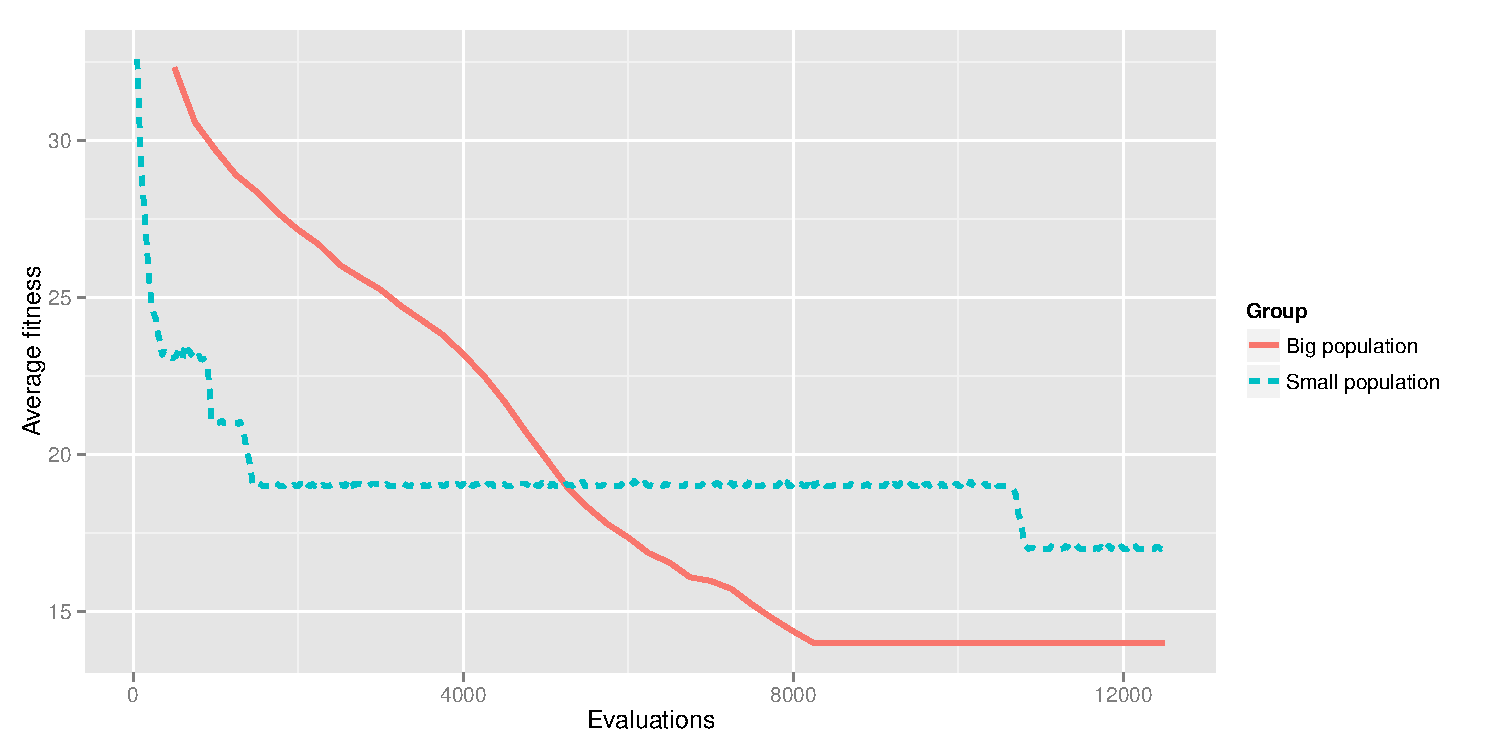
\includegraphics[width=0.65\textwidth] {./Irudiak/ga_graph_col_3-1}
}\qquad
\subfigure[Lortutako soluzioa]{
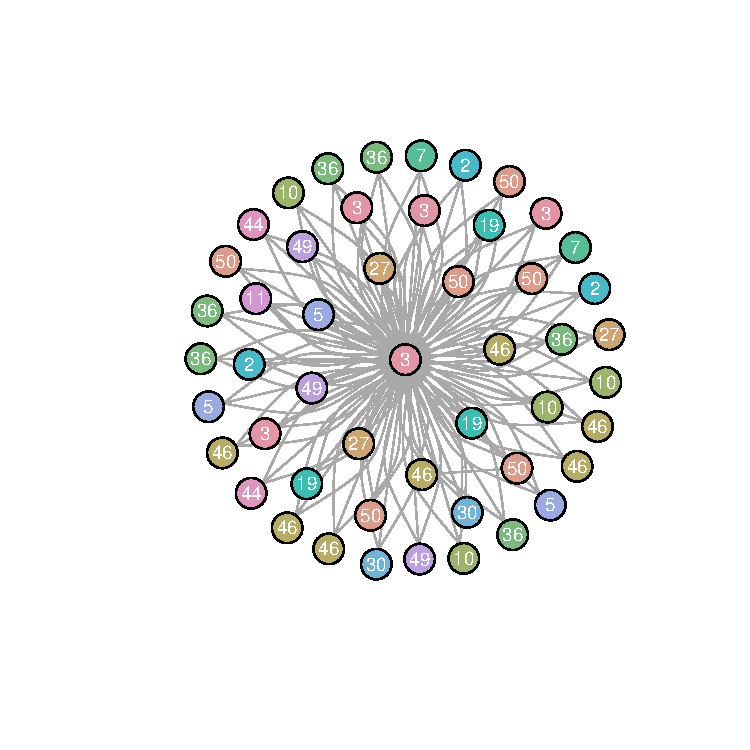
\includegraphics[width=0.30\textwidth] {./Irudiak/ga_graph_col_4-1}
}\\
\caption{Definitutako algoritmo genetikoaren progresioa \eng{graph coloring} problemaren instantzia batean batean, bi populazio tamaina ezberdin erabiliz. Ezkerrean, tamaina handiko populazioarekin lortutako soluzioa ikus daiteke.}\label{fig:ga_progress}
\end{figure}

Jarraian parametro hauek erabiliz algoritmo genetikoa exekutatzeko kodea ikus dezakegu.


\begin{knitrout}
\definecolor{shadecolor}{rgb}{1, 1, 1}\color{fgcolor}\begin{kframe}
\begin{alltt}
\hlstd{> }\hlstd{args} \hlkwb{<-} \hlkwd{list}\hlstd{()}
\hlstd{> }\hlstd{args}\hlopt{$}\hlstd{evaluate}             \hlkwb{<-} \hlstd{gcp}\hlopt{$}\hlstd{evaluate}
\hlstd{> }\hlstd{args}\hlopt{$}\hlstd{initial.population}   \hlkwb{<-} \hlstd{pop.small}
\hlstd{> }\hlstd{args}\hlopt{$}\hlstd{selectSubpopulation}  \hlkwb{<-} \hlstd{elitistSelection}
\hlstd{> }\hlstd{args}\hlopt{$}\hlstd{selection.ratio}      \hlkwb{<-} \hlnum{0.5}
\hlstd{> }\hlstd{args}\hlopt{$}\hlstd{selectCross}          \hlkwb{<-} \hlstd{tournamentSelection}
\hlstd{> }\hlstd{args}\hlopt{$}\hlstd{mutate}               \hlkwb{<-} \hlstd{factorMutation}
\hlstd{> }\hlstd{args}\hlopt{$}\hlstd{ratio}                \hlkwb{<-} \hlnum{0.1}
\hlstd{> }\hlstd{args}\hlopt{$}\hlstd{mutation.rate}        \hlkwb{<-} \hlnum{1} \hlopt{/} \hlkwd{length}\hlstd{(args}\hlopt{$}\hlstd{initial.population)}
\hlstd{> }\hlstd{args}\hlopt{$}\hlstd{cross}                \hlkwb{<-} \hlstd{kPointCrossover}
\hlstd{> }\hlstd{args}\hlopt{$}\hlstd{k}                    \hlkwb{<-} \hlnum{2}
\hlstd{> }\hlstd{args}\hlopt{$}\hlstd{non.valid}            \hlkwb{<-} \hlstr{"discard"}
\hlstd{> }\hlstd{args}\hlopt{$}\hlstd{resources}            \hlkwb{<-} \hlkwd{cResource}\hlstd{(}\hlkwc{evaluations}\hlstd{=}\hlnum{5} \hlopt{*} \hlstd{n}\hlopt{^}\hlnum{2}\hlstd{)}
\hlstd{> }
\hlstd{> }\hlstd{bga.small} \hlkwb{<-} \hlkwd{do.call}\hlstd{(basicGeneticAlgorithm, args)}
\hlstd{> }
\hlstd{> }\hlstd{args}\hlopt{$}\hlstd{initial.population}   \hlkwb{<-} \hlstd{pop.big}
\hlstd{> }\hlstd{args}\hlopt{$}\hlstd{mutation.rate}        \hlkwb{<-} \hlnum{1} \hlopt{/} \hlkwd{length}\hlstd{(args}\hlopt{$}\hlstd{initial.population)}
\hlstd{> }
\hlstd{> }\hlstd{bga.big} \hlkwb{<-} \hlkwd{do.call}\hlstd{(basicGeneticAlgorithm, args)}
\hlstd{> }
\hlstd{> }\hlkwd{plotProgress}\hlstd{(}\hlkwd{list}\hlstd{(}\hlstr{"Big population"}\hlstd{=bga.big,} \hlstr{"Small population"}\hlstd{=bga.small),} \hlkwc{size}\hlstd{=}\hlnum{1.1}\hlstd{)} \hlopt{+}
\hlstd{+ }  \hlkwd{labs}\hlstd{(}\hlkwc{y}\hlstd{=}\hlstr{"Average fitness"}\hlstd{)} \hlopt{+} \hlkwd{aes}\hlstd{(}\hlkwc{linetype}\hlstd{=Group)}
\end{alltt}
\end{kframe}
\end{knitrout}





\ref{fig:ga_progress} irudian bi populazio tamaina ezberdin erabiliz bilaketaren progresioa ikus daiteke. Populazioa txikia denean algoritmoak oso azkar konbergitzen du 19 kolore darabiltzan soluzio batera. Populazioko soluzio gehienak oso antzerakoak direnean soluzio berriak sortzeko bide bakarra mutazioa da, baina prozesu hori oso motela denez, grafikan ikus daiteke soluzioen bataz besteko \eng{fitness}a ez dela aldatzen. 

Populazioaren tamaina handitzen dugunean konbergentzia zailagoa da eta grafikan ikus daiteke helburu funtzioaren balioaren eboluzioa motelagoa izan arren, lortutako soluzioa hobea dela.

\begin{figure}[t]
\centering
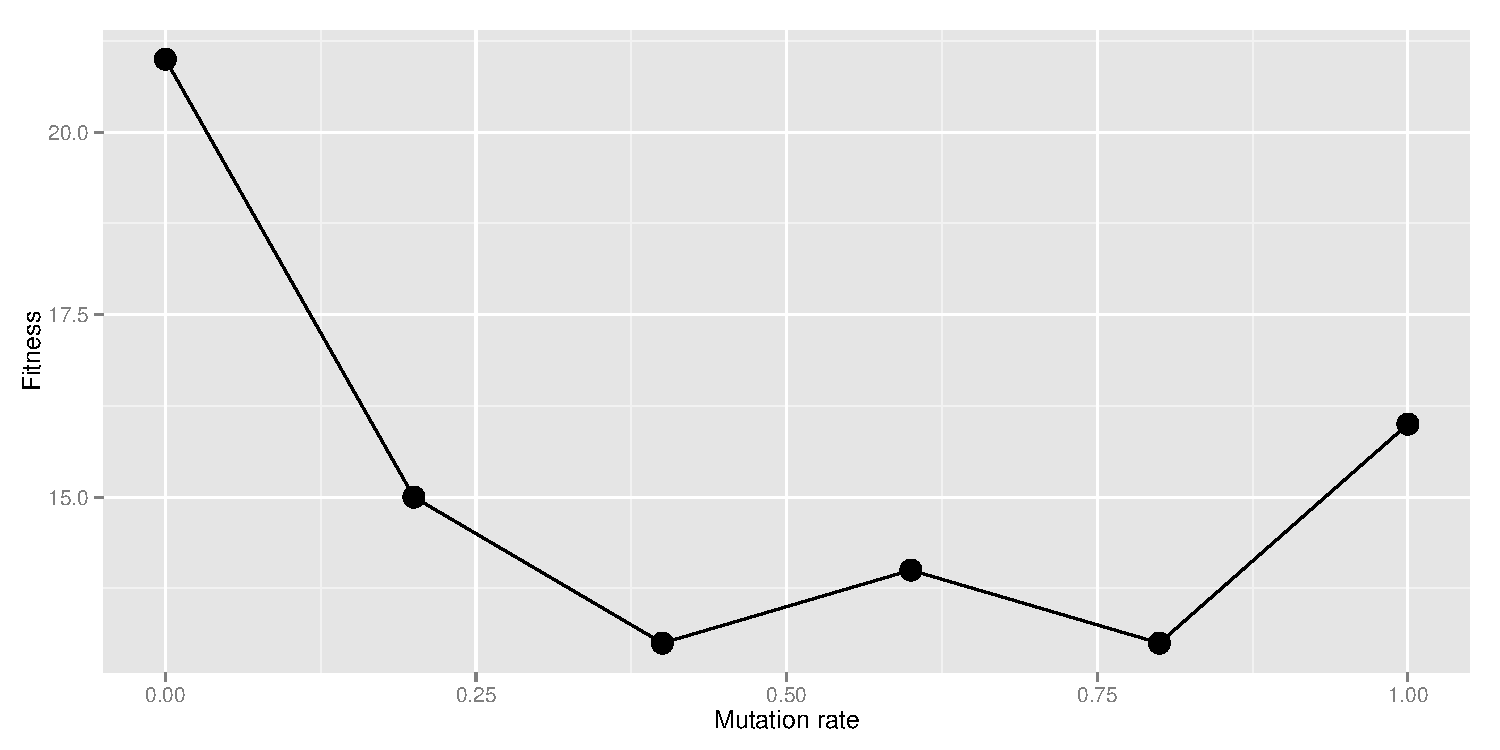
\includegraphics[width=0.75\textwidth] {./Irudiak/ga_mut_rate-1}
\caption{Mutazio probabilitatearen eragina algoritmo genetikoaren azken emaitzan. Irudian ikus daitekeen bezala, soluziorik onena ematen duen mutazio probabilitatearen balioa 0.5 inguruan dago (zehazki, 0.6). }\label{fig:ga_mutrate}
\end{figure}

Populazioaren tamaina ez ezik, beste hainbat parametrok ere eragin handia izan dezakete algoritmoaren emaitzan; esate baterako, mutazioaren probabilitatea. Adibide gisa, populazio tamaina txikia erabiliz mutazio probabilitate ezberdinak probatuko ditugu, eta, bakoitzarekin lortutako emaitzak alderatuko ditugu.

\begin{knitrout}
\definecolor{shadecolor}{rgb}{1, 1, 1}\color{fgcolor}\begin{kframe}
\begin{alltt}
\hlstd{> }\hlstd{args}\hlopt{$}\hlstd{initial.population}   \hlkwb{<-} \hlstd{pop.small}
\hlstd{> }\hlstd{args}\hlopt{$}\hlstd{verbose}              \hlkwb{<-} \hlnum{FALSE}
\hlstd{> }\hlstd{args}\hlopt{$}\hlstd{resources}            \hlkwb{<-} \hlkwd{cResource}\hlstd{(}\hlkwc{evaluations}\hlstd{=n}\hlopt{^}\hlnum{2}\hlstd{)}
\hlstd{> }
\hlstd{> }\hlstd{testMutProb} \hlkwb{<-} \hlkwa{function} \hlstd{(}\hlkwc{rate}\hlstd{) \{}
\hlstd{+ }  \hlstd{args}\hlopt{$}\hlstd{mutation.rate} \hlkwb{<-} \hlstd{rate}
\hlstd{+ }  \hlstd{res} \hlkwb{<-} \hlkwd{do.call}\hlstd{(basicGeneticAlgorithm, args)}
\hlstd{+ }  \hlkwd{return}\hlstd{(}\hlkwd{getEvaluation}\hlstd{(res))}
\hlstd{+ }\hlstd{\}}
\hlstd{> }
\hlstd{> }\hlstd{ratios} \hlkwb{<-} \hlkwd{seq}\hlstd{(}\hlnum{0}\hlstd{,}\hlnum{1}\hlstd{,}\hlnum{0.2}\hlstd{)}
\hlstd{> }\hlstd{evaluations} \hlkwb{<-} \hlkwd{sapply}\hlstd{(ratios ,} \hlkwc{FUN} \hlstd{= testMutProb)}
\hlstd{> }
\hlstd{> }\hlstd{df} \hlkwb{<-} \hlkwd{data.frame}\hlstd{(}\hlstr{"Mutation_rate"}\hlstd{=ratios,} \hlstr{"Fitness"}\hlstd{=evaluations)}
\hlstd{> }\hlkwd{ggplot}\hlstd{(df,} \hlkwd{aes}\hlstd{(}\hlkwc{x}\hlstd{=Mutation_rate,} \hlkwc{y}\hlstd{=Fitness))} \hlopt{+} \hlkwd{geom_line}\hlstd{()} \hlopt{+} \hlkwd{geom_point}\hlstd{(}\hlkwc{size}\hlstd{=}\hlnum{5}\hlstd{)} \hlopt{+}
\hlstd{+ }  \hlkwd{labs}\hlstd{(}\hlkwc{x}\hlstd{=}\hlstr{"Mutation rate"}\hlstd{)}
\end{alltt}
\end{kframe}
\end{knitrout}


\ref{fig:ga_mutrate} irudian lortutako emaitzak ikus daitezke. Grafikoak agerian uzten du mutazio probabilitate txikiegiak zein handiegiak ezartzea kaltegarria dela bilaketa prozesuarenzat, probabilitate egokiena 0.5 ingurukoa izanik. Jokabide honen zergatia bilatzen badugu, konturatzen gara probabilitate txikien kasuan emaitzak txarrak direla, populazioaren dibertsitatea txikia delako eta, ondorioz, konbergentzia goiztiarra ematen delako. Probabilitate handiekin berriz, arazoa justo kontrakoa izan daiteke, alegia, bilaketa ia ausazkoa dela eta beraz konbergentzia oso zaila dela. Hau egiaztatzeko, goiko experimentua errepika dezakezu ebaluazio kopuru maximoa handituz.

\subsection{Estimation of Distribution Algorithms}

Algoritmo genetikoetan uneko populazioa indibiduo berriak sortzeko erabiltzen da, naturan inspiratutako gurutzatze eta mutazio operadoreak aplikatuz.  Prozesu honen bitartez, populazioan dauden ezaugarriak mantentzea espero dugu. 

Zenbait ikertzailek ideia hau hartu eta ikuspuntu matematikotik birformulatu zuten. Honela, gurutzatze eta mutazioa erabili beharrean, eredu probabilistikoak erabiltzea proposatu zuten, populazioaren \hgl{esentzia} jasotzeko helburuarekin. Hauxe da, EDA -- \eng{Estimation of Distribution Algorithms} -- algoritmoen ideia nagusia. 

Algoritmo genetikoen eta EDA motako algoritmoen artean dagoen diferentzia bakarra indibiduo berriak sortzeko erabiltzen den estrategia da. Gurutzaketa eta mutazioa erabili beharrean, uneko populazioa eredu probabilistiko bat doitzeko erabiltzen da. Ondoren, eredu hori laginduko dugu behar adina indibiduo sortzeko.

EDA algoritmoen gakoa, beraz, eredu probabilistikoa da. Ildo honetan, esan beharra dago eredua soluzioen kodeketari lotuta dagoela, soluzio adierazpide bakoitzari probabilitate bat esleitu beharko diolako. 

Konplexutasun ezberdineko eredu probabilistikoen erabilera proposatu da literaturan, baina badago hurbilketa sinple bat oso hedatua dagoena: UMDA -- \eng{Univariate Marginal Distribution Algorithm} --. Kasu honetan soluzioaren osagaiak -- bektore bat bada, bere posizioak -- independenteak direla suposatuko dugu eta, hortaz, osagai bakoitzari dagokion probabilitate marjinala estimatuko dugu. Gero, indibiduoak sortzean soluzioaren osagaiak banan-banan aukeratuko ditugu probabilitate hauek jarraituz. 

Probabilitate marjinalak maneiatzeko \code{metaheuR} paketeko \code{UnivariateMarginals} objektua erabil dezakegu. Bere erabilera ikusteko, populazio txiki bat sortuko dugu eta probabilitate marginalak kalkulatuko ditugu. 

\begin{knitrout}
\definecolor{shadecolor}{rgb}{1, 1, 1}\color{fgcolor}\begin{kframe}
\begin{alltt}
\hlstd{> }\hlstd{population} \hlkwb{<-} \hlkwd{lapply}\hlstd{(}\hlnum{1}\hlopt{:}\hlnum{5}\hlstd{,}
\hlstd{+ }                     \hlkwc{FUN}\hlstd{=}\hlkwa{function}\hlstd{(}\hlkwc{x}\hlstd{) \{}
\hlstd{+ }                       \hlstd{res} \hlkwb{<-} \hlkwd{factor}\hlstd{(}\hlkwd{sample}\hlstd{(}\hlnum{1}\hlopt{:}\hlnum{3}\hlstd{,} \hlnum{10}\hlstd{,} \hlkwc{replace}\hlstd{=}\hlnum{TRUE}\hlstd{),} \hlkwc{levels}\hlstd{=}\hlnum{1}\hlopt{:}\hlnum{3}\hlstd{)}
\hlstd{+ }                       \hlkwd{return}\hlstd{(res)}
\hlstd{+ }                     \hlstd{\})}
\end{alltt}
\end{kframe}
\end{knitrout}

Orain, \code{univariateMarginals} funtzioa erabiliz probabilitate marginalak kalkulatuko ditugu:

\begin{knitrout}
\definecolor{shadecolor}{rgb}{1, 1, 1}\color{fgcolor}\begin{kframe}
\begin{alltt}
\hlstd{> }\hlstd{model} \hlkwb{<-} \hlkwd{univariateMarginals}\hlstd{(}\hlkwc{data}\hlstd{=population)}
\hlstd{> }\hlkwd{do.call}\hlstd{(rbind, population)}
\end{alltt}
\begin{verbatim}
##      [,1] [,2] [,3] [,4] [,5] [,6] [,7] [,8] [,9] [,10]
## [1,]    1    2    2    3    1    3    3    2    2     1
## [2,]    1    1    3    2    3    2    3    3    2     3
## [3,]    3    1    2    1    1    2    1    2    3     2
## [4,]    2    2    2    1    3    3    3    1    3     2
## [5,]    3    2    3    2    2    3    1    2    3     3
\end{verbatim}
\begin{alltt}
\hlstd{> }\hlstd{model}\hlopt{@}\hlkwc{prob.table}
\end{alltt}
\begin{verbatim}
##   [,1] [,2] [,3] [,4] [,5] [,6] [,7] [,8] [,9] [,10]
## 1  0.4  0.4  0.0  0.4  0.4  0.0  0.4  0.2  0.0   0.2
## 2  0.2  0.6  0.6  0.4  0.2  0.4  0.0  0.6  0.4   0.4
## 3  0.4  0.0  0.4  0.2  0.4  0.6  0.6  0.2  0.6   0.4
\end{verbatim}
\end{kframe}
\end{knitrout}

Sortutako soluzioek 10 elementu dituzte (10 posizioko bektore kategorikoak dira) eta populazioak 5 soluzio ditu. Lehenengo elementu edo posizioari erreparatzen badiogu, 5 soluzioetatik lehenengo biak 1 balioa dute, laugarrenak 2 balioa eta beste biak 3 balioa. Hortaz, elementu horretarako, 1 eta 3 balioen probabilitatea 0.4 izango da --$\frac{2}{5}$, alegia-- eta 2 balioaren probabilitatea 0.2 izango da, marginaleen taulan ikus daitekeen bezala.

Ikasitako eredu probabilistikoa soluzio berriak sortzeko erabil daiteke, posizioz-posizio dagokion marginala laginduz; laginketa \code{simulate} funtzioaren bidez egiten da.

\begin{knitrout}
\definecolor{shadecolor}{rgb}{1, 1, 1}\color{fgcolor}\begin{kframe}
\begin{alltt}
\hlstd{> }\hlkwd{simulate}\hlstd{(model,} \hlkwc{nsim}\hlstd{=}\hlnum{2}\hlstd{)}
\end{alltt}
\begin{verbatim}
## [[1]]
##  [1] 3 1 2 2 1 3 3 2 2 3
## Levels: 1 2 3
## 
## [[2]]
##  [1] 2 2 2 2 3 3 3 3 3 1
## Levels: 1 2 3
\end{verbatim}
\end{kframe}
\end{knitrout}

UMDA \code{basicEda} funtzioaren bidez exekutatu dezakegu eta, segidan, aurreko ataleko problema ebazteko erabiliko dugu. Horretarako, bakarrik hautespen operadoreak eta ereduak ikasteko funtzioak zehaztu behar ditugu --algoritmo genetikoekin komunak diren parametroez gain--.

\begin{knitrout}
\definecolor{shadecolor}{rgb}{1, 1, 1}\color{fgcolor}\begin{kframe}
\begin{alltt}
\hlstd{> }\hlstd{args} \hlkwb{<-} \hlkwd{list}\hlstd{()}
\hlstd{> }\hlstd{args}\hlopt{$}\hlstd{evaluate}             \hlkwb{<-} \hlstd{gcp}\hlopt{$}\hlstd{evaluate}
\hlstd{> }\hlstd{args}\hlopt{$}\hlstd{initial.population}   \hlkwb{<-} \hlstd{pop.small}
\hlstd{> }\hlstd{args}\hlopt{$}\hlstd{selectSubpopulation}  \hlkwb{<-} \hlstd{elitistSelection}
\hlstd{> }\hlstd{args}\hlopt{$}\hlstd{selection.ratio}      \hlkwb{<-} \hlnum{0.5}
\hlstd{> }\hlstd{args}\hlopt{$}\hlstd{learn}                \hlkwb{<-} \hlstd{univariateMarginals}
\hlstd{> }\hlstd{args}\hlopt{$}\hlstd{non.valid}            \hlkwb{<-} \hlstr{"discard"}
\hlstd{> }\hlstd{args}\hlopt{$}\hlstd{resources}            \hlkwb{<-} \hlkwd{cResource}\hlstd{(}\hlkwc{evaluations} \hlstd{= n}\hlopt{^}\hlnum{2}\hlstd{)}
\hlstd{> }
\hlstd{> }\hlstd{umda} \hlkwb{<-} \hlkwd{do.call}\hlstd{(basicEda, args)}
\hlstd{> }
\hlstd{> }\hlkwd{plotProgress}\hlstd{(umda,} \hlkwc{size}\hlstd{=}\hlnum{1.1}\hlstd{)} \hlopt{+}
\hlstd{+ }  \hlkwd{geom_line}\hlstd{(}\hlkwd{aes}\hlstd{(}\hlkwc{y}\hlstd{=Current_sol} \hlopt{+} \hlstd{Current_sd),} \hlkwc{col}\hlstd{=}\hlstr{"gray40"}\hlstd{,} \hlkwc{linetype}\hlstd{=}\hlnum{2}\hlstd{)} \hlopt{+}
\hlstd{+ }  \hlkwd{geom_line}\hlstd{(}\hlkwd{aes}\hlstd{(}\hlkwc{y}\hlstd{=Current_sol} \hlopt{-} \hlstd{Current_sd),} \hlkwc{col}\hlstd{=}\hlstr{"gray40"}\hlstd{,} \hlkwc{linetype}\hlstd{=}\hlnum{2}\hlstd{)} \hlopt{+}
\hlstd{+ }  \hlkwd{labs}\hlstd{(}\hlkwc{y}\hlstd{=}\hlstr{"Average fitness"}\hlstd{)}
\end{alltt}
\end{kframe}
\end{knitrout}

\begin{figure}[t]
\centering
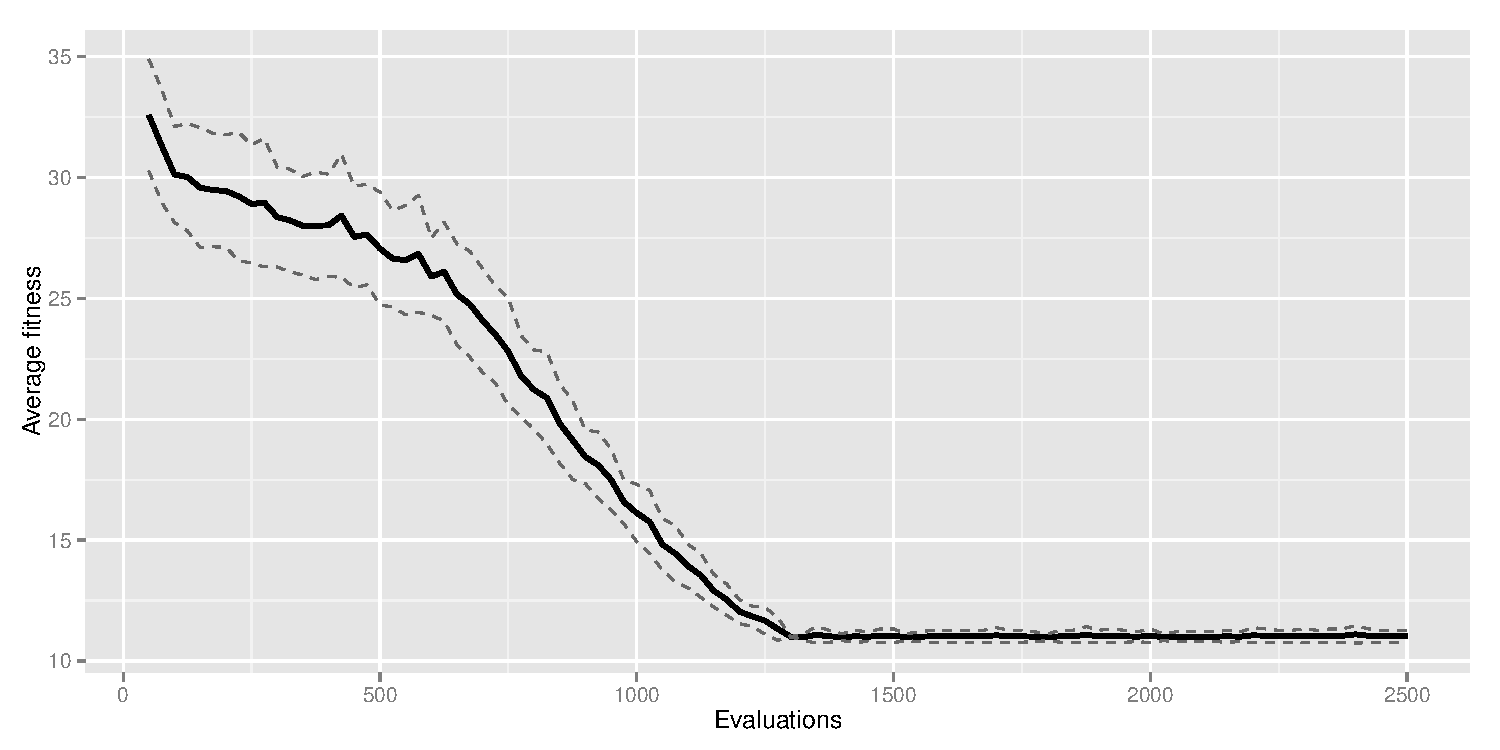
\includegraphics[width=0.75\textwidth] {./Irudiak/umda_gc-1}
\caption{UMDA algoritmoaren progresioa \eng{graph coloring} problemaren istantzia batean aplikatuta. Marra jarraituak populazioko soluzioen bataz-besteko \eng{fitness}a adierazten du; marra etenek, berriz, desbiderazio estandarra adierazten dute. Ikus daiteke populazioak konbergitzen duen heinean soluzioen \eng{fitness}aren aldakortasuna murrizten dela.}\label{fig:umda}
\end{figure}

Bilaketaren progresioa \ref{fig:umda} irudian erakusten da. Marra etenek populazioan dauden soluzioen \eng{fitness}aren desbiderapena erakusten dute eta marra jarraikiak, ordea, populazioko soluzioen fitness-aren batez-bestekoa. Populazioak eboluzionatu ahala, populazioaren dibertsitatea murrizten dela ikus dezakegu desbiderapenaren murrizketan erreparatuz. Amaieran, bilaketak 11 kolore darabiltzan soluzio batera konbergitzen du.

Marjinalak kalkulatzeko estrategia ia edozein bektore motarekin erabil daitezke zuzenean; alabaina, balio errealak baditugu, marjinalak zein probabilitate distribuzioarekin modelatuko ditugun erabaki beharko dugu aurrez. Aukera ezberdin asko daude baina ohiko distribuzio bat distribuzio normala da. Gainera, soluzioek murrizketak dituztenean, permutazioetan kasu, gauzak konplikatu egiten dira. 

Permutazio multzo bat izanik, posible da marjinalak bektore kategorikoekin bezala estimatzea baina, ondoren, eredua lagintzen dugunean ez ditugu halabeharrez permutazioak lortuko, balio errepikatuak ager baitaitezke. Hona hemen adibide bat:

\begin{knitrout}
\definecolor{shadecolor}{rgb}{1, 1, 1}\color{fgcolor}\begin{kframe}
\begin{alltt}
\hlstd{> }\hlstd{n} \hlkwb{<-} \hlnum{5}
\hlstd{> }\hlstd{generateRndPopulation} \hlkwb{<-} \hlkwd{lapply}\hlstd{(}\hlnum{1}\hlopt{:}\hlnum{50}\hlstd{,}
\hlstd{+ }                   \hlkwc{FUN}\hlstd{=}\hlkwa{function}\hlstd{(}\hlkwc{x}\hlstd{) \{}
\hlstd{+ }                     \hlstd{res} \hlkwb{<-} \hlkwd{factor}\hlstd{(}\hlkwd{as.numeric}\hlstd{(}\hlkwd{randomPermutation}\hlstd{(n)),} \hlkwc{levels}\hlstd{=}\hlnum{1}\hlopt{:}\hlstd{n)}
\hlstd{+ }                     \hlkwd{return}\hlstd{(res)}
\hlstd{+ }                   \hlstd{\})}
\hlstd{> }\hlstd{perm.umda} \hlkwb{<-} \hlkwd{univariateMarginals}\hlstd{(generateRndPopulation)}
\hlstd{> }\hlkwd{simulate}\hlstd{(perm.umda)}
\end{alltt}
\begin{verbatim}
## [[1]]
## [1] 3 2 1 4 4
## Levels: 1 2 3 4 5
\end{verbatim}
\end{kframe}
\end{knitrout}

Arazo hau sahiesteko, soluzio berriak lagintzean, permutazioak dakarzten murrizketak aintzat hartu behar dira. Honela, laginketa prozesuan lehenengo elementua ausaz aukeratuko dugu, zuzenean marjinala erabiliz. 

\begin{knitrout}
\definecolor{shadecolor}{rgb}{1, 1, 1}\color{fgcolor}\begin{kframe}
\begin{alltt}
\hlstd{> }\hlstd{marginals} \hlkwb{<-} \hlstd{perm.umda}\hlopt{@}\hlkwc{prob.table}
\hlstd{> }\hlstd{remaining} \hlkwb{<-} \hlnum{1}\hlopt{:}\hlstd{n}
\hlstd{> }\hlstd{probabilities} \hlkwb{<-} \hlstd{marginals[,}\hlnum{1}\hlstd{]}
\hlstd{> }\hlstd{new.element} \hlkwb{<-} \hlkwd{sample}\hlstd{(remaining,} \hlkwc{size}\hlstd{=}\hlnum{1}\hlstd{,} \hlkwc{prob}\hlstd{=probabilities)}
\hlstd{> }\hlstd{new.solution} \hlkwb{<-} \hlstd{new.element}
\end{alltt}
\end{kframe}
\end{knitrout}

Ondoren, bigarren elementua aukeratu aurretik, lehenengo posiziorako aukeratu dugun elementua kendu beharko dugu aukera posibleetatik eta marjinalak honen arabera eguneratu--erabili dugun elementuaren probabilitatea kendu eta normalizatu, gelditzen diren elementuen probabilitateen batura 1 izan dadin--:

\begin{knitrout}
\definecolor{shadecolor}{rgb}{1, 1, 1}\color{fgcolor}\begin{kframe}
\begin{alltt}
\hlstd{> }\hlstd{id} \hlkwb{<-} \hlkwd{which}\hlstd{(remaining} \hlopt \hlstd{new.element)}
\hlstd{> }\hlstd{remaining} \hlkwb{<-} \hlstd{remaining [}\hlopt{-}\hlstd{id]}
\hlstd{> }\hlstd{marginals} \hlkwb{<-} \hlstd{marginals[}\hlopt{-}\hlstd{id, ]}
\hlstd{> }\hlstd{probabilities} \hlkwb{<-} \hlstd{marginals[,} \hlnum{2}\hlstd{]}
\hlstd{> }\hlstd{probabilities} \hlkwb{<-} \hlstd{probabilities} \hlopt{/} \hlkwd{sum}\hlstd{(probabilities)}
\hlstd{> }\hlstd{new.element} \hlkwb{<-} \hlkwd{sample}\hlstd{(remaining,} \hlkwc{size}\hlstd{=}\hlnum{1}\hlstd{,} \hlkwc{prob}\hlstd{=probabilities)}
\hlstd{> }\hlstd{new.solution} \hlkwb{<-} \hlkwd{c}\hlstd{(new.solution, new.element)}
\end{alltt}
\end{kframe}
\end{knitrout}

Estrategia berbera aplikatzen dugu 3. eta 4. elementuak erauzteko.

\begin{knitrout}
\definecolor{shadecolor}{rgb}{1, 1, 1}\color{fgcolor}\begin{kframe}
\begin{alltt}
\hlstd{> }\hlstd{id} \hlkwb{<-} \hlkwd{which}\hlstd{(remaining} \hlopt \hlstd{new.element)}
\hlstd{> }\hlstd{remaining} \hlkwb{<-} \hlstd{remaining [}\hlopt{-}\hlstd{id]}
\hlstd{> }\hlstd{marginals} \hlkwb{<-} \hlstd{marginals[}\hlopt{-}\hlstd{id, ]}
\hlstd{> }\hlstd{probabilities} \hlkwb{<-} \hlstd{marginals[,} \hlnum{3}\hlstd{]}
\hlstd{> }\hlstd{probabilities} \hlkwb{<-} \hlstd{probabilities} \hlopt{/} \hlkwd{sum}\hlstd{(probabilities)}
\hlstd{> }\hlstd{new.element} \hlkwb{<-} \hlkwd{sample}\hlstd{(remaining,} \hlkwc{size}\hlstd{=}\hlnum{1}\hlstd{,} \hlkwc{prob}\hlstd{=probabilities)}
\hlstd{> }\hlstd{new.solution} \hlkwb{<-} \hlkwd{c}\hlstd{(new.solution, new.element)}
\hlstd{> }
\hlstd{> }\hlstd{id} \hlkwb{<-} \hlkwd{which}\hlstd{(remaining} \hlopt \hlstd{new.element)}
\hlstd{> }\hlstd{remaining} \hlkwb{<-} \hlstd{remaining [}\hlopt{-}\hlstd{id]}
\hlstd{> }\hlstd{marginals} \hlkwb{<-} \hlstd{marginals[}\hlopt{-}\hlstd{id, ]}
\hlstd{> }\hlstd{probabilities} \hlkwb{<-} \hlstd{marginals[,} \hlnum{3}\hlstd{]}
\hlstd{> }\hlstd{probabilities} \hlkwb{<-} \hlstd{probabilities} \hlopt{/} \hlkwd{sum}\hlstd{(probabilities)}
\hlstd{> }\hlstd{new.element} \hlkwb{<-} \hlkwd{sample}\hlstd{(remaining,} \hlkwc{size}\hlstd{=}\hlnum{1}\hlstd{,} \hlkwc{prob}\hlstd{=probabilities)}
\hlstd{> }\hlstd{new.solution} \hlkwb{<-} \hlkwd{c}\hlstd{(new.solution, new.element)}
\end{alltt}
\end{kframe}
\end{knitrout}

Amaitzeko, permutazioaren azken elementua definitzeko, soberan geratzen den  elementua aukeratuko dugu zuzenean.

\begin{knitrout}
\definecolor{shadecolor}{rgb}{1, 1, 1}\color{fgcolor}\begin{kframe}
\begin{alltt}
\hlstd{> }\hlstd{id} \hlkwb{<-} \hlkwd{which}\hlstd{(remaining} \hlopt \hlstd{new.element)}
\hlstd{> }\hlstd{remaining} \hlkwb{<-} \hlstd{remaining [}\hlopt{-}\hlstd{id]}
\hlstd{> }\hlstd{new.solution} \hlkwb{<-} \hlkwd{c}\hlstd{(new.solution, remaining)}
\hlstd{> }\hlstd{new.solution}
\end{alltt}
\begin{verbatim}
## [1] 4 3 5 1 2
\end{verbatim}
\end{kframe}
\end{knitrout}

Prozesu honekin probabilitate marjinalak erabil daitezke permutazioak sortzeko baina arazo bat dauka: eredua lagintzen dugun bakoitzean probabilitateak aldatzen ditugu eta, hortaz, lagintzen duguna ez da zehazki populaziotik ikasi dugun eredua. Beste era batean esanda, populaziotik ateratako \hgl{esentzia} galdu dezakegu. Hau ez gertatzeko, permutazio espazioetan definitutako probabilitate distribuzioak erabil ditzakegu; esate baterako, Mallows eredua, \code{metaheuR} paketean dagoen \code{MallowsModel} objektuak inplementatzen duena.


\section{Swarm Intelligence}\label{sec:swarm}

Eboluzioaren bidez natura indibiduoen diseinua \hgl{optimizatzeko} gai da; alabaina, naturan optimizazio estrategiak beste hainbat egoeratan ere ageri dira. Adibide gisa, animalia sozialen portaera eta jokabideak optimizazio algoritmoak sortzeko inspirazio iturri izan dira sarritan. 

Zenbait espezietako indibiduoak --intsektuak, batik bat-- banan-banan hartuta, oso izaki sinpleak dira baina, taldeka lan egiten dutenean, ataza konplexuak era oso eraginkorrean burutzeko gai dira. Esate baterako, inurriak eta erleak elikagai-iturri onenak aukeratzeko gai dira eta, hauen kapazitate eta egoeraren arabera, ingurunea esploratzen duten indibiduen kopurua egokitzen dute iturri berriak lortu ahal izateko; era berean, bizitzeko toki egokienak aukeratzeko gai dira.

Honelako bizidun multzoetan erabakiak ez dira era zentralizatuan hartzen --alegia, ez dago agintzen duen \hgl{nagusi}\negthickspace{}rik --. Beraz, mekanismo sinple batzuk jarraituz eta, batez ere, haien arteko komunikazioari esker, kolonia bateko indibiduoak elkar antolatzeko gai dira, inolako koordinazio zentralizaturik gabe.

Mota honetako portaerak dira zehazki \eng{swarm intelligence} deritzon arloaren inspirazio iturria. Mota honetako algoritmoak lehenengo aldiz 1988. urtean robotika arloan proposatu ziren \cite{beni1988}, baina urte gutxi batzuetan optimizazio mundura hedatu ziren. Honela, 90. hamarkadan inurri kolonien optimizazioa --\eng{Ant Colony Optimization}, ingelesez-- proposatu zen \cite{dorigo1992, dorigo1996}.

Hurrengo bi ataletan \eng{swarm intelligence} arloan dauden bi algoritmo ezagunenak aztertuko ditugu, inurri kolonien optimizazioa eta \eng{particle swarm optimization}.


\subsection{\eng{Ant Colony Optimization}}

Inurriek, elikagai-iturri bat topatzen dutenean, inurritegitik bertara dagoen biderik motzena topatzeko gaitasuna dute. Inurri bakar batek ezin du horrelakorik egin baina, taldeka, komunikazio mekanismo sinpleei esker, ataza konplexu hau burutzeko gai dira. Erabiltzen den komunikazio mota zeharkakoa da, inurriek jariatzen duten molekula mota berezi baten bidez gauzatzen dena:  feromona. 

Inurriak toki batetik bestera mugitzean, beste inurriek detektatu dezaketen feromona-lorratz bat uzten dute. Inurriak, haien kolonia-kideak utzitako feromona lorratzak detektatzeko gai dira eta honetaz baliatzen dira haien ibilbideak aukeratzeko. Hala, geroz eta feromona gehiago egon bide batean, orduan eta probabilitate handiagoa dago bertatik igarotzen diren inurriak bide horretatik jarraitzeko. Bestalde, inurri batek elikagai-iturri bat topatzen duenean, bidetik uzten duen feromona kopurua iturriaren kalitatearen arabera egokitzen du; geroz eta kalitate handiagoa, orduan eta feromona kopuru handiagoa jariatzen du. Azkenik, feromona lurrunkorra da, alegia, denborarekin baporatu egiten da.

\begin{figure}[t]
\centering
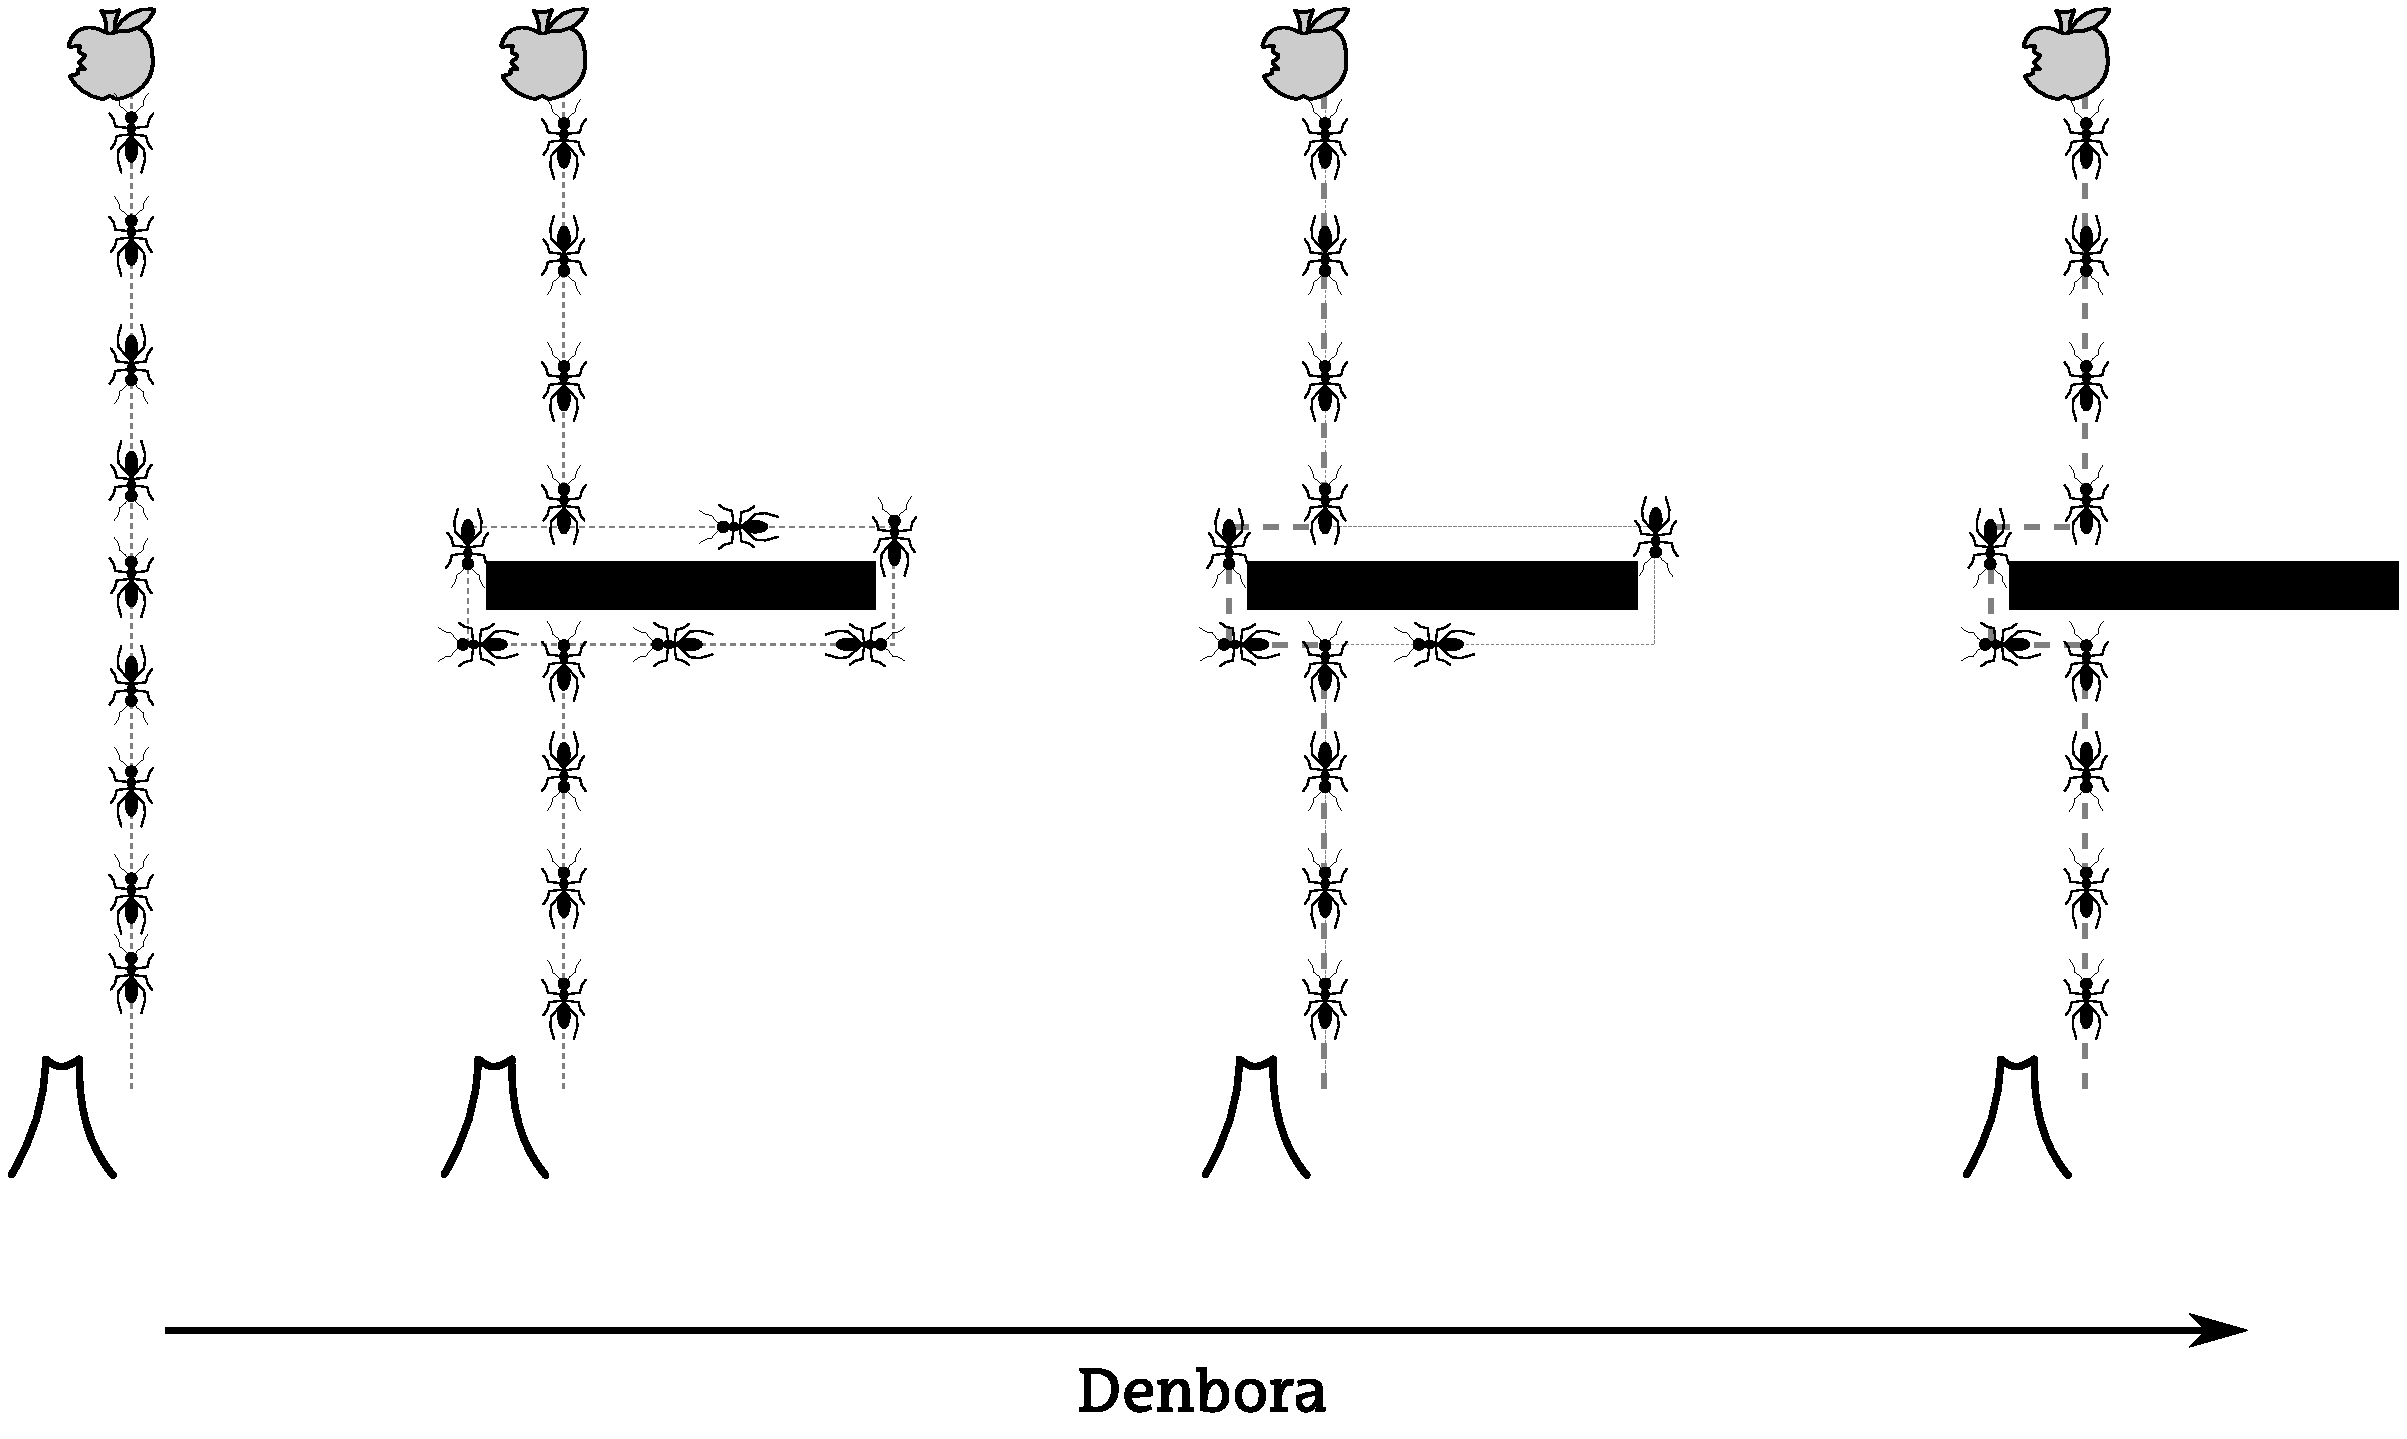
\includegraphics[width=0.75\linewidth]{./Irudiak/ants}
\caption{Feromonaren erabilera. Hasierako egoeran biderik motzena feromona lorratzak zehazten du. Bidea mozten dugunean, inurriek, eskuinetik ala ezkerretik joatea erabaki beharko dute. Hasieran erabaki hau probabilitate berdinarekin hartuko dute, feromonarik ez baitago ez ezkerrean eta ez eskuinean ere. Alabaina, eskuineko bidea luzeagoa da eta, ezkerreko bidearekin alderatuta, inurri-fluxua txikiagoa izango da, inurriek denbora gehiago beharko baitute elikadura-iturrira joan eta etorria egiteko. Arrazoi honegatik, denbora igaro ahala, eskumako lorratza ahuldu egingo da eta ezkerrekoa, berriz, indartu. Guzti honek puntu honetara iristen diren inurrien erabakia baldintzatuko du, ezkerreko bidea aukeratzeko joera areagotuz eta bi bideen arteko diferentzia handituz. Denbora nahikoa igaro ezkero eskuineko lorratza guztiz desagertuko da eta inurriak bide motzena bakarrik aukeratuko dute.}
\label{fig:ants}
\end{figure}


Arau sinple hauek erabiliz inurriak elikagai-iturri onenak aukeratzeko gai dira; are gehiago, elikagai eta inurritegiaren arteko biderik motzena ere topatu dezakete. Mekanismo honen funtzionamendua hobeto ulertzeko\ref{fig:ants} irudiari erreparatu diezaiokegu. Hasieran, bide motzena feromona lorratzaren bidez markaturik dator. Bidea moztean, eskuineko eta ezkerreko bideetan ez dago feromonarik eta, hortaz, inurri batzuk eskumatik eta beste batzuk ezkerretik joango dira, probabilitate berdinarekin. Ezkerreko bidea motzagoa denez, denbora berdinean inurri gehiago igaroko dira, ezkerreko bideako feromona-lorratza indartsuagoa bilakatuz. Denbora igaro ahala, datozen inurriak ezkerretik joateko joera handiagoa izango dute eta honek bide hau are gehiago indartuko du. Eskumako bidean lorratza apurka-apurka baporatu egingo da eta, denbora nahikoa igarotzen bada, zeharo galduko da. 

Laburbilduz, inurriek ez dituzte bi bideak konparatzen baina, hala eta guztiz ere, azkenean, bide motza soilik erabiltzea lortzen dute. \eng{Ant Colony Optimization} (ACO) deritzon metaheuristikak inurrien portaera hau hartzen du intuiziotzat eta inurri artifizialak erabiltzen ditu optimizazio problemaren soluzioak sortzeko. Soluzio hauek ez dira edonolakoak izango, izan ere, naturan bezalaxe, aurretik igarotako inurriek utzitako lorratzak jarraituz sortuko dira. 

Lorratzak feromona ereduen bidez adierazten dira eta, eredu hauek optimizazio algoritmoaren pausu bakoitzean bi eratan eguneratzen dira. Alde batetik, inurriek sortutako soluzioen kalitatea --hots, helburu funtzioaren balioa-- feromona kopurua areagotzeko erabiltzen da. Bestalde, iterazioz iterazio feromona kopurua murriztuko da, naturan ematen den baporazioa simulatuz. Feronoma eredua zehazteko, pausu bakoitzean feronomaren areagotzea eta murrizketa nola egin erabaki behar dugu.

Beraz, bi gauza behar dira ACO algoritmo bat diseinatzeko: feromona eredu bat eta soluzioak sortzeko algoritmo bat. Soluzioak sortzeko era sinpleena osagaietan oinarritzen den algoritmo eraikitzaile bat erabiltzea da. Ikus dezagun hau adibide bat.

Demagun MIS problema ebatzi nahi dugula. Problema honetarako soluzioak bektore bitarren bidez kodetzen ditugu eta, hortaz, bektoreen posizioak soluzioen osagaitzat har ditzakegu. Posizio bakoitzak bi balio posible har ditzake, 0 edo 1. Soluzio bat sortzeko, inurri artifizial bakoitzak, hasteko, soluzio bektorearen lehenengo posizioko balioa 0 edo 1 den aukeratu beharko du. Horretarako, uneko feromona kopurua hartuko du aintzat, probabilitate handiagoa esleituz feromona gehiago duen aukerari; behin lehenengo posizioko balioa finkaturik, bigarren posizioan jarriko du arreta da eta, lehenengo pausuan bezala, balio bat (0 edo 1) probabilistikoki aukeratuko du feromona kopuruan oinarrituz. Prozesu bera soluzio osoa sortu arte errepikatuko da.

Adibide honetan, feromona eredua matrize sinple baten bidez inplementa daiteke, zutabe bakoitzak soluzio bektorearen posizio bat adierazten duelarik. Bestalde, matrizeak bi errenkada izango ditu, posizio bakoitzean 0 eta 1 balioek duten feromona kopurua gordetzeko. 

Feromona eredu honen erabilera argitzeko MIS problema erabili beharrean, antzerakoa den beste problema bat erabiliko dugu: \eng{Minimum Dominating Set} (MDS). Laburki azalduz, grafo bat emanda, nodoen azpimultzo bat menderatze-multzoa da --\eng{dominating set}, ingelesez-- baldin eta azpimultzoan ez dauden nodo guztiak, gutxienez, azpimultzoko nodo bati konektatuta badaude. Grafo bat emanik, MDS problema, kardinalitate minimoko menderatze-multzoa topatzean datza. \ref{fig:MDS} irudian problema honetarako hiru soluzio ikus daitezke. 

Lehenik, ausazko grafo bat erakiko dugu MDS problemaren instantzia bat definitzeko.

\begin{figure}[t]
\subfigure[Soluzio hau bideraezina da, menderatze-multzoa ez baita]{
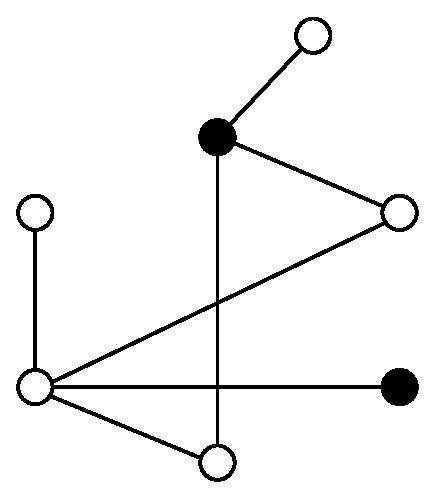
\includegraphics[width=0.3\textwidth] {./Irudiak/MDS_not}
}\qquad
\subfigure[4 tamainako menderatze-multzoa]{
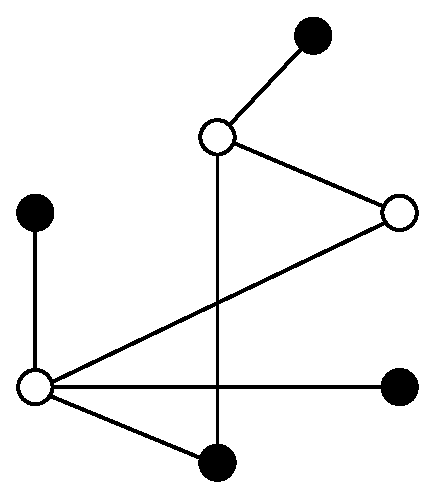
\includegraphics[width=0.3\textwidth] {./Irudiak/MDS_4}
}\qquad
\subfigure[2 tamainako menderatze-multzoa]{
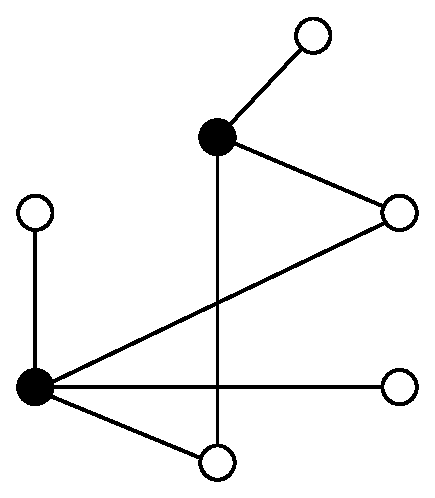
\includegraphics[width=0.3\textwidth] {./Irudiak/MDS_2}
}\\
\caption{Irudiak MDS problemarako 3 soluzio jasotzen ditu --beltzez adierazita dauden nodoak--. Lehenengoa (ezkerrean dagoena), ez da bideragarria, soluziokoa ez den nodo bat ez baitago konektatuta soluzioko nodo batekin ere. Bigarren soluzioa bideragarria da, baina ez optimoa. Azken soluzioa optimoa da, ez baitago 1 tamainako soluzio bideragarririk.}\label{fig:MDS}
\end{figure}


\begin{knitrout}
\definecolor{shadecolor}{rgb}{1, 1, 1}\color{fgcolor}\begin{kframe}
\begin{alltt}
\hlstd{> }\hlstd{n} \hlkwb{<-} \hlnum{10}
\hlstd{> }\hlstd{rnd.graph} \hlkwb{<-} \hlkwd{aging.ba.game} \hlstd{(n,} \hlnum{0.5}\hlstd{,} \hlnum{0}\hlstd{,} \hlnum{2}\hlstd{,} \hlkwc{directed}\hlstd{=}\hlnum{FALSE}\hlstd{)}
\hlstd{> }\hlstd{mdsp} \hlkwb{<-} \hlkwd{mdsProblem}\hlstd{(}\hlkwc{graph}\hlstd{=rnd.graph)}
\end{alltt}
\end{kframe}
\end{knitrout}

Bigarren pausuan, feromona eredua eraikitzeko matrizea hasieratu behar dugu. Feromona eredu mota hau \code{metaheuR} paketeko \code{VectorPheromone} klasearen bidez inplementaturik dago. Ohikoena balio finko batekin hasieratzea da. Era honetan osagai guztiak balio berdina dute eta, beraz, aukera posible guztien probabilitatea berdina izango da. Gogoratu gure adibidean feromona ereduaren matrizeak bi errenkada dituela, soluzioak bektore bitarrak direlako.

\begin{knitrout}
\definecolor{shadecolor}{rgb}{1, 1, 1}\color{fgcolor}\begin{kframe}
\begin{alltt}
\hlstd{> }\hlstd{init.trail} \hlkwb{<-} \hlkwd{matrix} \hlstd{(}\hlkwd{rep}\hlstd{(}\hlnum{1}\hlstd{,} \hlnum{2}\hlopt{*}\hlstd{n),} \hlkwc{ncol}\hlstd{=n)}
\hlstd{> }\hlstd{evaporation} \hlkwb{<-} \hlnum{0.1}
\hlstd{> }\hlstd{pheromones} \hlkwb{<-} \hlkwd{vectorPheromone}\hlstd{(}\hlkwc{binary}\hlstd{=}\hlnum{TRUE}\hlstd{,} \hlkwc{initial.trail}\hlstd{=init.trail,}
\hlstd{+ }                              \hlkwc{evaporation.factor}\hlstd{=evaporation)}
\hlstd{> }\hlstd{pheromones}\hlopt{@}\hlkwc{trail}
\end{alltt}
\begin{verbatim}
##      [,1] [,2] [,3] [,4] [,5] [,6] [,7] [,8] [,9] [,10]
## [1,]    1    1    1    1    1    1    1    1    1     1
## [2,]    1    1    1    1    1    1    1    1    1     1
\end{verbatim}
\end{kframe}
\end{knitrout}

Goiko kodean ikus daitekeen bezala, feromona eredua guztiz zehazteko, badago beste parametro bat finkatu behar dena: \code{evaporation.factor} parametroa. Parametro hau feromonaren lurrunketarekin dago erlazionatuta eta matrizean dauden balioak pausu bakoitzean zenbat murriztuko diren adierazten du; balio hau kontutan izanik, baporazioa \code{evaporate} funtzioa erabiliz egiten da.

\begin{knitrout}
\definecolor{shadecolor}{rgb}{1, 1, 1}\color{fgcolor}\begin{kframe}
\begin{alltt}
\hlstd{> }\hlkwd{evaporate}\hlstd{(pheromones)}
\hlstd{> }\hlstd{pheromones}\hlopt{@}\hlkwc{trail}
\end{alltt}
\begin{verbatim}
##      [,1] [,2] [,3] [,4] [,5] [,6] [,7] [,8] [,9] [,10]
## [1,]  0.9  0.9  0.9  0.9  0.9  0.9  0.9  0.9  0.9   0.9
## [2,]  0.9  0.9  0.9  0.9  0.9  0.9  0.9  0.9  0.9   0.9
\end{verbatim}
\begin{alltt}
\hlstd{> }\hlkwd{evaporate}\hlstd{(pheromones)}
\hlstd{> }\hlstd{pheromones}\hlopt{@}\hlkwc{trail}
\end{alltt}
\begin{verbatim}
##      [,1] [,2] [,3] [,4] [,5] [,6] [,7] [,8] [,9] [,10]
## [1,] 0.81 0.81 0.81 0.81 0.81 0.81 0.81 0.81 0.81  0.81
## [2,] 0.81 0.81 0.81 0.81 0.81 0.81 0.81 0.81 0.81  0.81
\end{verbatim}
\end{kframe}
\end{knitrout}

Esan dugun bezala, inurriek feromona ereduak soluzioak eraikitzeko erabiltzen dute. Soluzioak \code{buildSolution} funtzioaren bitartez egiten da.

\begin{knitrout}
\definecolor{shadecolor}{rgb}{1, 1, 1}\color{fgcolor}\begin{kframe}
\begin{alltt}
\hlstd{> }\hlkwd{buildSolution}\hlstd{(pheromones,} \hlnum{1}\hlstd{)}
\end{alltt}
\begin{verbatim}
## [[1]]
##  [1]  TRUE  TRUE FALSE FALSE  TRUE  TRUE FALSE  TRUE  TRUE FALSE
\end{verbatim}
\end{kframe}
\end{knitrout}

Inurriek ingurunetik ibiltzen diren heinean feromona uzten dute eta, era berean, inurri artifizialek soluzioak eraikitzen dutenean feromona kopurua handitzen dute; ereduaren eguneraketa hau \code{updateTrail} funtzioa erabiliz egiten da.

\begin{knitrout}
\definecolor{shadecolor}{rgb}{1, 1, 1}\color{fgcolor}\begin{kframe}
\begin{alltt}
\hlstd{> }\hlstd{solution} \hlkwb{<-} \hlkwd{buildSolution}\hlstd{(pheromones,} \hlnum{1}\hlstd{)[[}\hlnum{1}\hlstd{]]}
\hlstd{> }\hlstd{eval} \hlkwb{<-} \hlstd{mdsp}\hlopt{$}\hlkwd{evaluate}\hlstd{(solution)}
\hlstd{> }\hlstd{eval}
\end{alltt}
\begin{verbatim}
## [1] 4
\end{verbatim}
\begin{alltt}
\hlstd{> }\hlkwd{updateTrail}\hlstd{(}\hlkwc{object}\hlstd{=pheromones,} \hlkwc{solution}\hlstd{=solution,} \hlkwc{value}\hlstd{=eval)}
\hlstd{> }\hlstd{pheromones}\hlopt{@}\hlkwc{trail}
\end{alltt}
\begin{verbatim}
##      [,1] [,2] [,3] [,4] [,5] [,6] [,7] [,8] [,9] [,10]
## [1,] 4.81 4.81 0.81 0.81 4.81 4.81 4.81 0.81 0.81  4.81
## [2,] 0.81 0.81 4.81 4.81 0.81 0.81 0.81 4.81 4.81  0.81
\end{verbatim}
\end{kframe}
\end{knitrout}

Ikus daitekeen bezala, zutabe bakoitzean errenkada bati (inurriak aukeratutako balioari dagokionari, hain zuzen) soluzioaren helburu funtzioaren balioa gehitu zaio, inurriek utzitako lorratza irudikatuz. 

Elementu guzti hauekin, ACO sinple bat sor dezakegu. Lehenik, problema berri bat --handiagoa-- sortuko dugu.

\begin{knitrout}
\definecolor{shadecolor}{rgb}{1, 1, 1}\color{fgcolor}\begin{kframe}
\begin{alltt}
\hlstd{> }\hlstd{n} \hlkwb{<-} \hlnum{100}
\hlstd{> }\hlstd{rnd.graph} \hlkwb{<-} \hlkwd{aging.ba.game}\hlstd{(n,} \hlnum{0.5}\hlstd{,} \hlnum{0}\hlstd{,} \hlnum{3}\hlstd{,} \hlkwc{directed}\hlstd{=}\hlnum{FALSE}\hlstd{)}
\hlstd{> }\hlstd{mdsp} \hlkwb{<-} \hlkwd{mdsProblem}\hlstd{(}\hlkwc{graph}\hlstd{=rnd.graph)}
\hlstd{> }\hlstd{init.trail} \hlkwb{<-} \hlkwd{matrix} \hlstd{(}\hlkwd{rep}\hlstd{(}\hlnum{1}\hlstd{,} \hlnum{2}\hlopt{*}\hlstd{n),} \hlkwc{ncol}\hlstd{=n)}
\hlstd{> }\hlstd{pheromones} \hlkwb{<-} \hlkwd{vectorPheromone}\hlstd{(}\hlkwc{binary}\hlstd{=}\hlnum{TRUE}\hlstd{,} \hlkwc{initial.trail}\hlstd{=init.trail,}
\hlstd{+ }                              \hlkwc{evaporation.factor}\hlstd{=evaporation)}
\end{alltt}
\end{kframe}
\end{knitrout}

Orain, 500 inurri simulatuko ditugu; bakoitzak soluzio bat sortuko du eta egindako \hgl{bidean} feromona utziko du. Algoritmoaren pausu bakoitzean inurri bat simulatuko dugu eta haren ibilbidea amaitzean feromona \hgl{lurrundu} egigo dugu.

\begin{knitrout}
\definecolor{shadecolor}{rgb}{1, 1, 1}\color{fgcolor}\begin{kframe}
\begin{alltt}
\hlstd{> }\hlstd{num.ant} \hlkwb{<-} \hlnum{500}
\hlstd{> }\hlstd{sol.evaluations} \hlkwb{<-} \hlkwd{vector}\hlstd{()}
\hlstd{> }\hlkwa{for} \hlstd{(ant} \hlkwa{in} \hlnum{1}\hlopt{:}\hlstd{num.ant) \{}
\hlstd{+ }  \hlstd{solution} \hlkwb{<-} \hlstd{mdsp}\hlopt{$}\hlkwd{correct}\hlstd{(}\hlkwd{buildSolution}\hlstd{(pheromones,} \hlnum{1}\hlstd{)[[}\hlnum{1}\hlstd{]])}
\hlstd{+ }  \hlstd{eval} \hlkwb{<-} \hlstd{mdsp}\hlopt{$}\hlkwd{evaluate}\hlstd{(solution)}
\hlstd{+ }  \hlkwd{updateTrail}\hlstd{(pheromones, solution, eval)}
\hlstd{+ }  \hlkwd{evaporate}\hlstd{(pheromones)}
\hlstd{+ }  \hlstd{sol.evaluations} \hlkwb{<-} \hlkwd{c}\hlstd{(sol.evaluations, eval)}
\hlstd{+ }\hlstd{\}}
\end{alltt}
\end{kframe}
\end{knitrout}

\begin{figure}
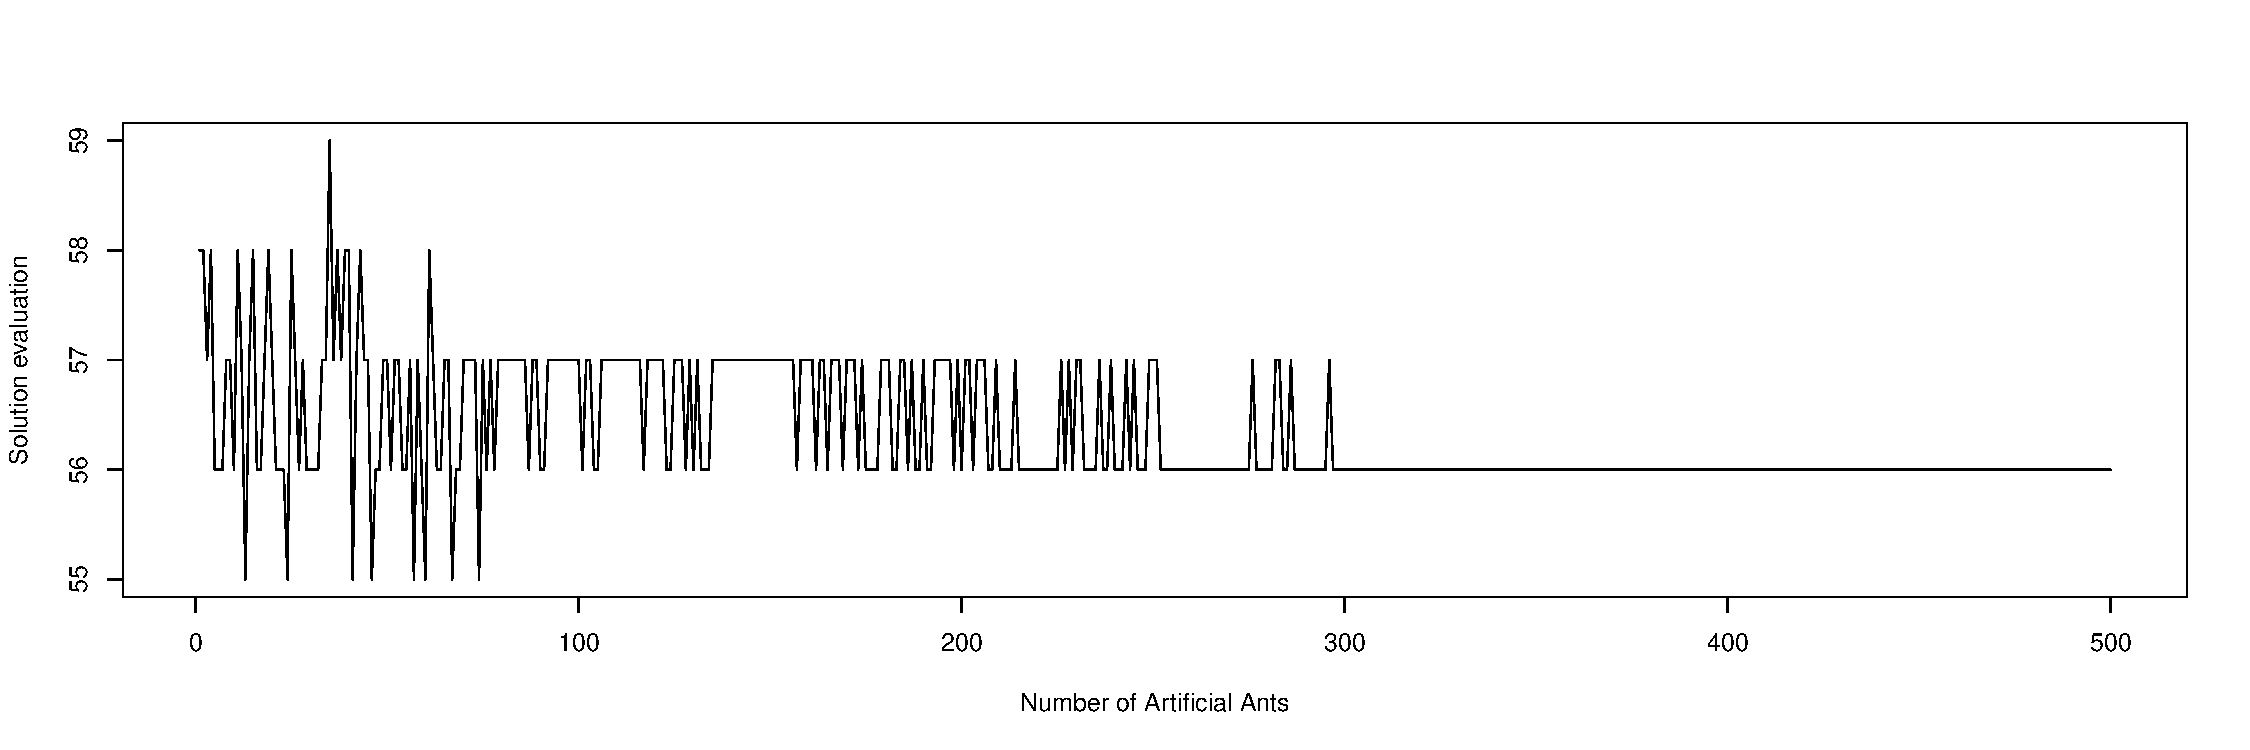
\includegraphics[width=\textwidth]{./Irudiak/ACO_MDS_8-1}
\caption{ACO sinplearen eboluzioa MDS problema batean.}\label{fig:simple_aco}
\end{figure}



\ref{fig:simple_aco} irudiak algoritmoaren eboluzioa erakusten du. Irudian, lehenengo inurriek sortutako soluzioen helburu funtzioaren balioak oso ezberdinak direla ikus daiteke. Alabaina, simulatutako inurri kopurua handitzen den heinean bariantza murriztu egiten da eta, amaieran, prozedurak soluzio bakar batera konbergitzen du. Edonola ere, soluzio hori ez da hasieran lortutakoak baino hobea. 

Portaera hau sakonago aztertu ezkero ondokoa ondorioztatzen da: nahiz eta naturan honela gertatu, optimizazioaren ikuspegitik, inurri guztiek feromona eredua eguneratzea ez da hurbilketarik onena. Hori dela eta, normalean beste estrategia bat erabili ohi da. Inurriak banan-banan simulatu ordez, tamaina zehatz bateko inurri-kolonia  bat sortzen da eta, iterazio bakoitzean, inurritegiko inurri guztiek sortutako soluzioetatik bakar bat erabiliko da feromona kopurua eguneratzeko. Soluzio bakar hau aukeratzeko bi estrategia ezberdin erabil daitezke:

\begin{itemize}
\item Iterazioko soluziorik onena aukeratu- Inurriek uneko iterazioan sortutako soluzioetatik onena aukeratzen da eta soluzio hori bakarrik erabiltzen da feromona kopurua eguneratzeko. Kasu honetan helburu funtzioaren arabera egitea ez da beharrezkoa, bakarrik soluziorik onena erabiltzen baita eguneraketan. Hori dela eta, ohikoa da balio finko bat erabiltzea.
\item Bilaketa prozesu osoan topatutako soluziorik aukeratu- Hainbat kasutan, bilaketa soluzio on baten inguruan areagotzea interesatuko zaigu. Kasu horietan, feromona ereduaren eguneraketa bilake prozesu osoan zehar topatu den soluziorik onena erabiliz egin daiteke. Aurreko puntuan bezala, eguneraketak ez du zertan  helburu funtzioaren balioarekiko proportzionala izan.
\end{itemize}


\begin{ifalgorithm}[t]
\begin{ifpseudo}{Inurri-kolonien algoritmoa}
\item \In\ \texttt{build\_solution}, \texttt{evaporate}, \texttt{add\_pheromone }, \texttt{initalize\_matrix} eta \texttt{stop\_criterion} operadoreak
\item \In\ \texttt{k\_size} koloniaren tamaina
\item \Out\ \texttt{opt\_solution}
\item \texttt{pheromone\_matrix} = \texttt{initialize\_matrix()}
\item \While !\texttt{stop\_criterion()}
\item \T{\textbf{for} \texttt{i} \textbf{in} 1:\texttt{k\_size}}
\item \TT{\texttt{solution} = \texttt{build\_solution(pheromone\_matrix)}}
\item \TT{\texttt{pheromone\_matrix} = \texttt{add\_pheromone(pheromone\_matrix,solution)}}
\item \TT{\If \texttt{solution} \texttt{opt\_solution} baino hobea da}
\item \TTT{\texttt{opt\_solution}=\texttt{solution}}
\item \TT{\EIf}
\item \T{\Done}
\item \T{\texttt{pheromone\_matrix} = \texttt{evaporate(pheromone\_matrix)}}
\item \Done
\end{ifpseudo}
\caption{Inurri-kolonien algoritmoaren sasikodea}\label{alg:ant}
\end{ifalgorithm}


Aldaketa honekin oinarrizko ACO algoritmoaren sasikodea defini dezakegu (ikusi \ref{alg:ant} algoritmoa). \code{basicAco} funtzioak Oinarrizko ACO-a inplementatzen du eta, hortaz, lehen sortutako MDS problema ebazteko erabil dezakegu. Ohiko parametroaz gain, \code{basicAco} argumentu hauek zehaztu behar dira.


\begin{itemize}
\item \code{nants} - Kolonia zenbat inurri artifizialek osatuko duten.
\item \code{pheromones} - Feromona eredua.
\item \code{update.sol} - Nola eguneratuko dugun feromona eredua. Hiru aukera daude: \code{'best.it'}, iterazio bakoitzean sortutako soluziorik onena erabili; \code{'best.all'}, bilaketan zehar lortutako soluziorik onena erabili edo \code{'all'}, sortutako soluzio guztietaz baliatu.
\item \code{update.value} - Balio bat finkatzen bada, eguneraketa guztietan feromona balio hori gehitzen zaio ereduari; \code{NULL} bada, helburu funtzioa erabiltzen da. Kontutan hartu problema batzuetan helburu funtzioak negatiboak direla eta feromona eredu batzuetan balio positiboak eta negatiboak ezin direla nahastu, arazoak egon daitezkeelako probabilitateak kalkulatzean. Hori dela eta, helburu funtzioaren zeinua kontutan hartu behar da feromona eredua hasieratzerakoan.
\end{itemize}

\begin{knitrout}
\definecolor{shadecolor}{rgb}{1, 1, 1}\color{fgcolor}\begin{kframe}
\begin{alltt}
\hlstd{> }\hlstd{args} \hlkwb{<-} \hlkwd{list}\hlstd{()}
\hlstd{> }\hlstd{args}\hlopt{$}\hlstd{evaluate}         \hlkwb{<-} \hlstd{mdsp}\hlopt{$}\hlstd{evaluate}
\hlstd{> }\hlstd{args}\hlopt{$}\hlstd{nants}            \hlkwb{<-} \hlnum{5}
\hlstd{> }
\hlstd{> }\hlstd{init.value}    \hlkwb{<-} \hlnum{1}
\hlstd{> }\hlstd{initial.trail} \hlkwb{<-} \hlkwd{matrix}\hlstd{(}\hlkwd{rep}\hlstd{(init.value,} \hlnum{2}\hlopt{*}\hlstd{n),} \hlkwc{nrow}\hlstd{=}\hlnum{2}\hlstd{)}
\hlstd{> }\hlstd{evapor}        \hlkwb{<-} \hlnum{0.1}
\hlstd{> }\hlstd{pher}          \hlkwb{<-} \hlkwd{vectorPheromone}\hlstd{(}\hlkwc{binary}\hlstd{=}\hlnum{TRUE}\hlstd{,} \hlkwc{initial.trail}\hlstd{=initial.trail,}
\hlstd{+ }                                 \hlkwc{evaporation.factor}\hlstd{=evapor)}
\hlstd{> }\hlstd{args}\hlopt{$}\hlstd{pheromones}   \hlkwb{<-} \hlstd{pher}
\hlstd{> }\hlstd{args}\hlopt{$}\hlstd{update.sol}   \hlkwb{<-} \hlstr{"best.it"}
\hlstd{> }\hlstd{args}\hlopt{$}\hlstd{update.value} \hlkwb{<-} \hlstd{init.value} \hlopt{/} \hlnum{10}
\hlstd{> }\hlstd{args}\hlopt{$}\hlstd{non.valid}    \hlkwb{<-} \hlstr{"correct"}
\hlstd{> }\hlstd{args}\hlopt{$}\hlstd{valid}        \hlkwb{<-} \hlstd{mdsp}\hlopt{$}\hlstd{is.valid}
\hlstd{> }\hlstd{args}\hlopt{$}\hlstd{correct}      \hlkwb{<-} \hlstd{mdsp}\hlopt{$}\hlstd{correct}
\hlstd{> }
\hlstd{> }\hlstd{args}\hlopt{$}\hlstd{resources}    \hlkwb{<-} \hlkwd{cResource}\hlstd{(}\hlkwc{iterations}\hlstd{=}\hlnum{100}\hlstd{)}
\hlstd{> }\hlstd{args}\hlopt{$}\hlstd{verbose}      \hlkwb{<-} \hlnum{FALSE}
\hlstd{> }
\hlstd{> }\hlstd{results.aco} \hlkwb{<-} \hlkwd{do.call}\hlstd{(basicAco, args)}
\hlstd{> }\hlkwd{plotProgress}\hlstd{(results.aco)} \hlopt{+} \hlkwd{labs}\hlstd{(}\hlkwc{y}\hlstd{=}\hlstr{"Average evaluation"}\hlstd{)}
\end{alltt}
\end{kframe}
\end{knitrout}

\begin{figure}
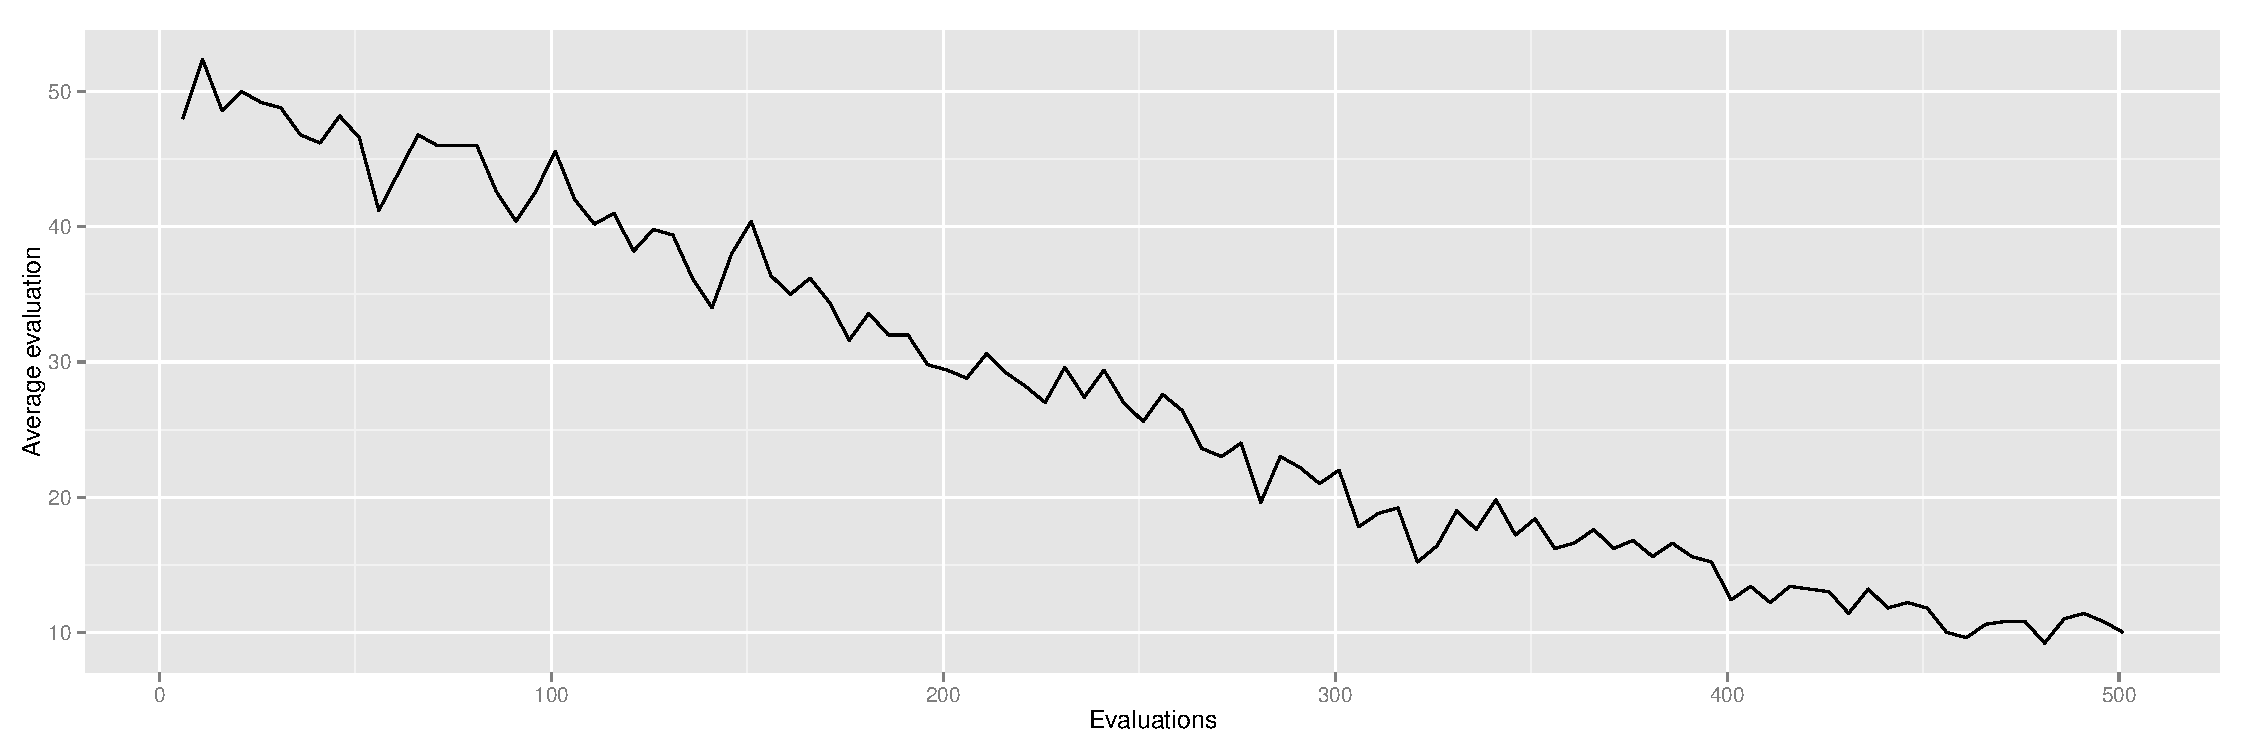
\includegraphics[width=\textwidth]{./Irudiak/ACO_MDS_10-1}
\caption{Oinarrizko ACO algoritmoaren eboluzioa MDS problema batean.}\label{fig:basic_aco}
\end{figure}

\ref{fig:basic_aco} irudiak oinarrizko ACO algoritmoaren progresioa irudikatzen du. Algoritmo honek, lehen inplementatu dugun ACO sinpleak aztertzen duen soluzio kopuru berdina aztertzen du baina, aurrekoa ez bezala, iterazioz iterazio soluzioa hobetuz doa. Grafikoan batazbesteko \eng{fitness}-ak bariabilidade handia duela ikus daiteke. Hau oso kolonia txikia erabili dugulako da --5 inurri bakarrik--. Balio hori handitzen badugu, prograsioa leunagoa izango da --eta, ziurrenik, emaitzak hobeak izango dira--, baina ebaluazio gehiago beharko ditugu.

ACO algoritmoen mamia soluzioen eraikuntza da eta, hortaz, soluzioen osagaien definizioa oso garrantzitsua da; osagaiek ez badute problemaren izaera kontutan hartzen, feromona ereduak ez du soluzioen informazioa behar bezala jasoko eta zentzua galduko du. Hau agerian gelditzen da jarraian dagoen adibidean.

Demagun LOP problema bat ebazteko ACO algoritmo bat erabili nahi dugula. Problema honetarako soluzioak permutazioen bidez kodetzen ditugunez, kodeketa mota honentzat egokia den feromona eredu bat behar dugu. Lehen ideia bazala, bektoreekin erabilitako eredu bera erabil dezakegu, soluzioen eraikuntzan permutazioak sortzeko behar diren aldaketak egiten baditugu betiere. Hau da, feronoma eredua matrize karratu batean gordeko dugu. Bertan, soluzioen posizio bakoitzeko (errenkadak) balio posible bakoitzari (zutabeak) dagokion feromona kopurua gordeko dugu. Gero, soluzioak osatzerakoan, urrats bakoitzean, aurretik aukeratu gabeko balioetatik bat aukertuko dugu, bakoitzaren feromona kopurua kontutan hartuz, noski. Eredu honek UMDA definitzeko erabili genuen matrizearen antzerako bat erabiltzen du. 

Dena dela, hau ez da feronoma eredu posible bakarra. TSP probleman ikusi genuen permutazioek grafo osoko ziklo Hamiltoniarrak adierazten dituztela. Hau da, $n$ nodoko grafo oso bat izanik, edozein permutaziok $n$ nodoak behin eta soilik behin bisitatzen dituen ibilbide bat adierazten du. Beraz, permutazioak osatzeko, nodoak lotzen dituzten ertzak erabil ditzakegu.

Ideia hau erabiliz beste feromona eredu bat plantea dezakegu. Eredu honek ere matrize karratu bat erabiliko du, baina matrizearen interpretazioa --eta, hortaz, soluzioen eraikuntza-- ezberdina da. Kasu honetan, matrizeak grafoaren ertzak adierazten ditu. Alegia, matrizearen $(i,j)$ posizioan $i$ nodotik $j$ nodorako bideari dagokion feromona kopurua gordeko dugu. Adibidez, 3421 permutazioari dagozkion matrizeko posizioak $(3,4); (4,2)$ eta $(2,1)$ dira --problemaren arabera, $(1,3)$ posizioa ere erabiltzea interesgarria izan daiteke, baina guk ez dugu aintzat hartuko gure adibidean--.

Bi eredu hauek \code{metaheuR} librutegian inplementaturik daude, \code{PermuPosPheromone} eta  \code{PermuLinkPheromone} objektuetan. Jarraian, bi eredu hauek LOP problema bat ebazteko erabiliko ditugu eta emaitzak alderatuko ditugu.

\begin{knitrout}
\definecolor{shadecolor}{rgb}{1, 1, 1}\color{fgcolor}\begin{kframe}
\begin{alltt}
\hlstd{> }\hlstd{n} \hlkwb{<-} \hlnum{100}
\hlstd{> }\hlstd{rnd.mat} \hlkwb{<-} \hlkwd{matrix}\hlstd{(}\hlkwd{round}\hlstd{(}\hlkwd{runif}\hlstd{(n}\hlopt{^}\hlnum{2}\hlstd{)}\hlopt{*}\hlnum{100}\hlstd{), n)}
\hlstd{> }\hlstd{lop}     \hlkwb{<-} \hlkwd{lopProblem}\hlstd{(}\hlkwc{matrix}\hlstd{=rnd.mat)}
\hlstd{> }
\hlstd{> }\hlstd{args} \hlkwb{<-} \hlkwd{list}\hlstd{()}
\hlstd{> }\hlstd{args}\hlopt{$}\hlstd{evaluate} \hlkwb{<-} \hlstd{lop}\hlopt{$}\hlstd{evaluate}
\hlstd{> }\hlstd{args}\hlopt{$}\hlstd{nants}    \hlkwb{<-} \hlnum{15}
\hlstd{> }
\hlstd{> }\hlstd{init.value}    \hlkwb{<-} \hlnum{1}
\hlstd{> }\hlstd{initial.trail} \hlkwb{<-} \hlkwd{matrix}\hlstd{(}\hlkwd{rep}\hlstd{(init.value, n}\hlopt{^}\hlnum{2} \hlstd{), n)}
\hlstd{> }\hlstd{evapor}        \hlkwb{<-} \hlnum{0.9}
\hlstd{> }\hlstd{pher}          \hlkwb{<-} \hlkwd{permuLinkPheromone}\hlstd{(}\hlkwc{initial.trail}\hlstd{=initial.trail,}
\hlstd{+ }                                    \hlkwc{evaporation.factor}\hlstd{=evapor)}
\hlstd{> }\hlstd{args}\hlopt{$}\hlstd{pheromones}   \hlkwb{<-} \hlstd{pher}
\hlstd{> }\hlstd{args}\hlopt{$}\hlstd{update.sol}   \hlkwb{<-} \hlstr{"best.it"}
\hlstd{> }\hlstd{args}\hlopt{$}\hlstd{update.value} \hlkwb{<-} \hlstd{init.value} \hlopt{/} \hlnum{10}
\hlstd{> }\hlstd{args}\hlopt{$}\hlstd{resources}    \hlkwb{<-} \hlkwd{cResource}\hlstd{(}\hlkwc{iterations}\hlstd{=}\hlnum{250}\hlstd{)}
\hlstd{> }\hlstd{args}\hlopt{$}\hlstd{verbose}      \hlkwb{<-} \hlnum{FALSE}
\hlstd{> }
\hlstd{> }\hlstd{aco.links} \hlkwb{<-} \hlkwd{do.call}\hlstd{(basicAco, args)}
\hlstd{> }
\hlstd{> }\hlstd{args}\hlopt{$}\hlstd{pheromones} \hlkwb{<-} \hlkwd{permuPosPheromone}\hlstd{(initial.trail, evapor)}
\hlstd{> }\hlstd{aco.pos} \hlkwb{<-} \hlkwd{do.call}\hlstd{(basicAco, args)}
\hlstd{> }
\hlstd{> }\hlkwd{plotProgress}\hlstd{(}\hlkwd{list}\hlstd{(}\hlstr{"Position"}\hlstd{=aco.pos,} \hlstr{"Link"}\hlstd{=aco.links))}
\end{alltt}
\end{kframe}
\end{knitrout}

\begin{figure}
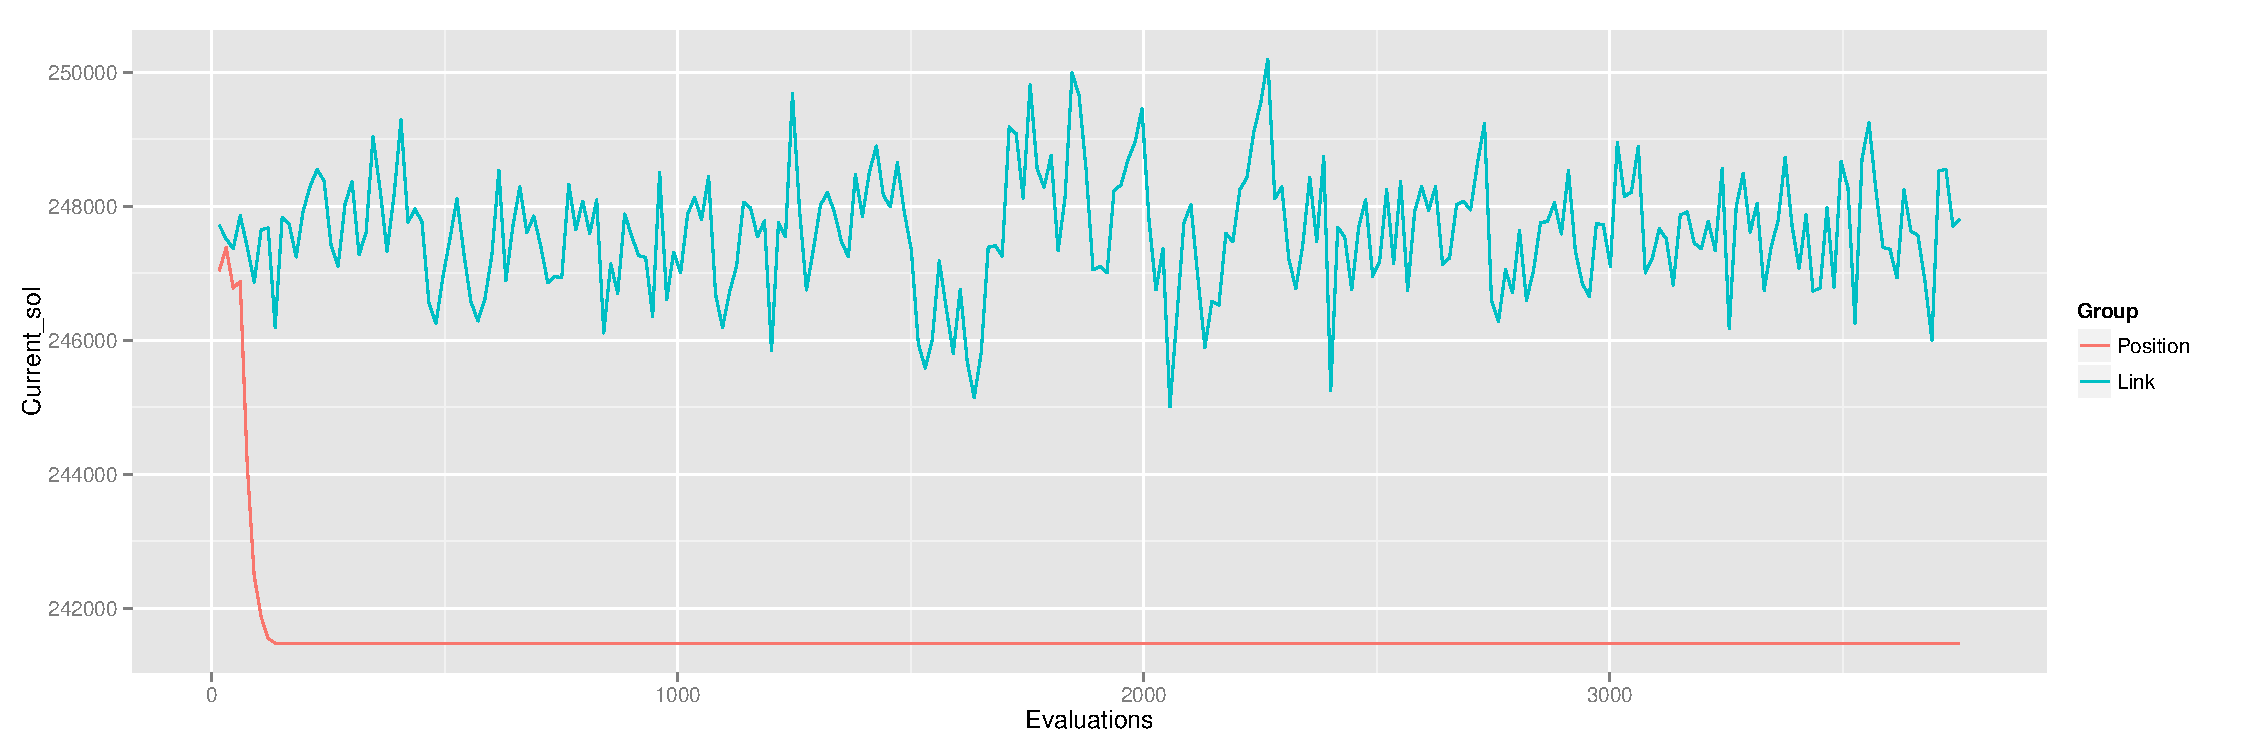
\includegraphics[width=\textwidth]{./Irudiak/ACO_LOP-1}
\caption{Oinarrizko ACO algoritmoaren eboluzioa LOP problema batean.}\label{fig:aco_lop}
\end{figure}

\ref{fig:aco_lop} irudiak esperimentuaren emaitza erakusten du. Grafikan argi ikus daiteke noden arteko loturak soluzioen osagaitzat hartzen direnean, bilaketak ez duela aurrera egiten. Soluzioaren ssagaiak posizioak direnean, berriz, iterazioz iterazio soluzioa hobetu egiten da. Honen arrazoia sinplea da: LOP probleman, soluzioko posizio absolutuak dira aspektu garrantzitsuena, eta ez zein elementu dagoen zeinen ondoan.

\begin{figure}
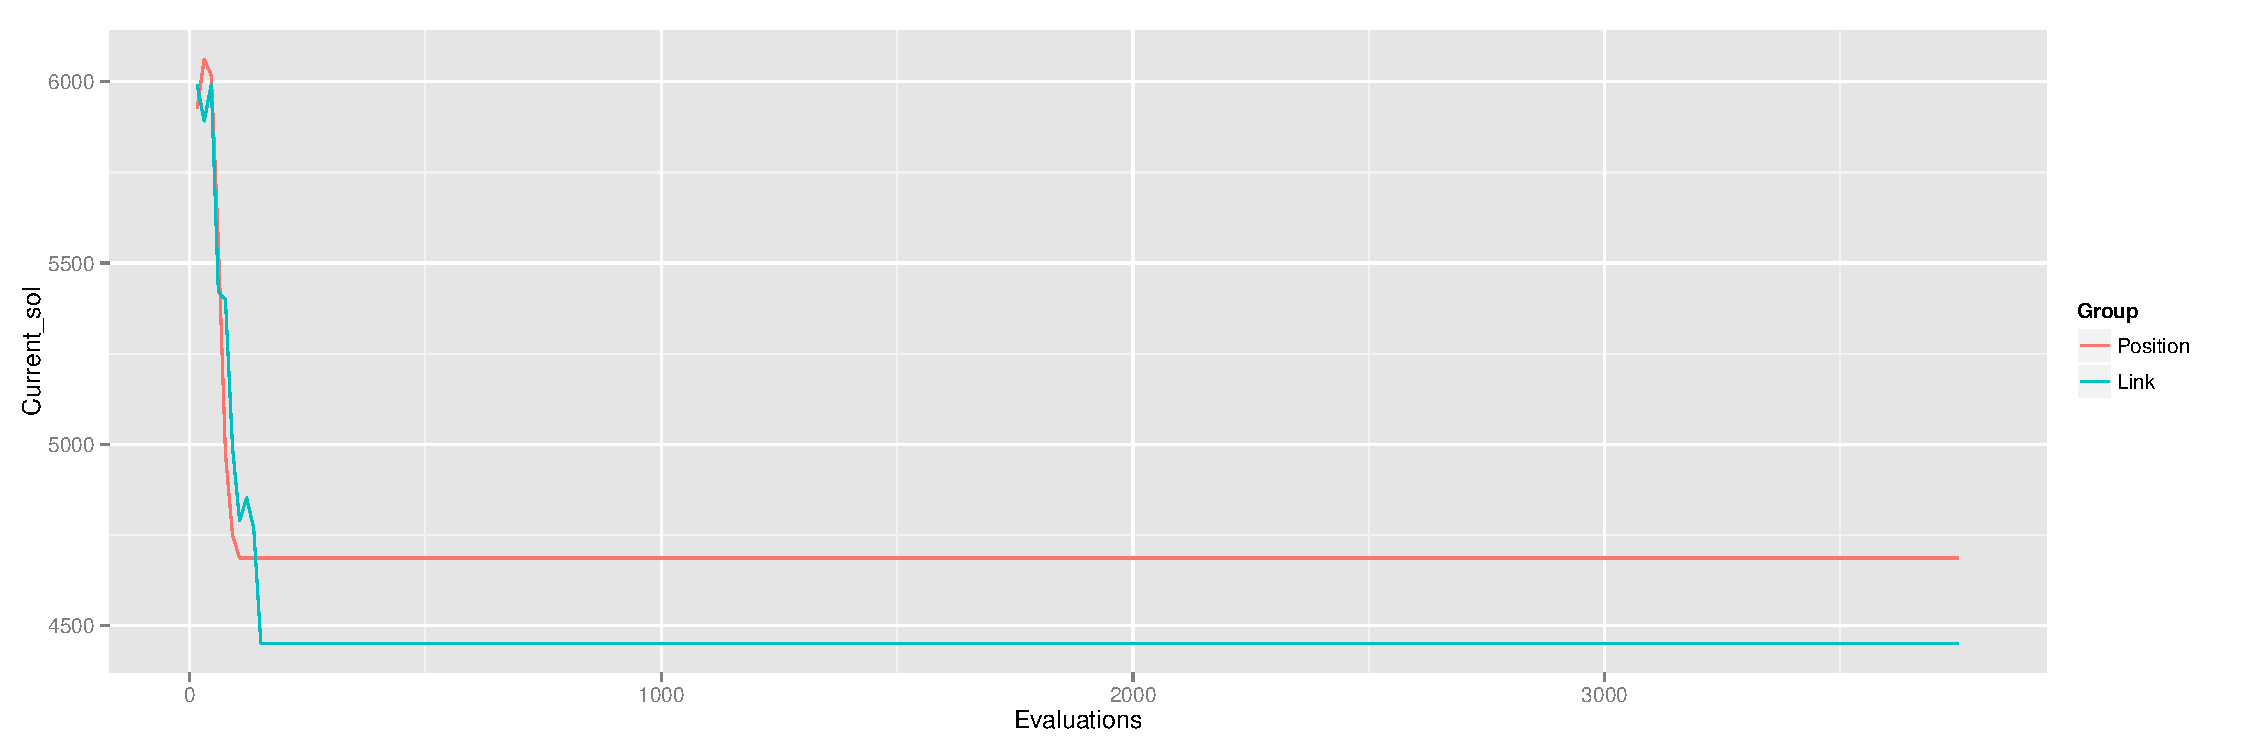
\includegraphics[width=\textwidth]{./Irudiak/ACO_TSP-1}
\caption{Oinarrizko ACO algoritmoaren eboluzioa TSP problema batean.}\label{fig:aco_tsp}
\end{figure}

TSP problemarako, ordea, ertzetan oinarritzen den eredua egokia da, izan ere, zein hiritik zein hirira joan behar dugun interesatzen zaigu. Jarraian hau frogatzeko esperimentu bat egingo dugu; emaitzak \ref{fig:aco_tsp} irudian daude.


\begin{knitrout}
\definecolor{shadecolor}{rgb}{1, 1, 1}\color{fgcolor}\begin{kframe}
\begin{alltt}
\hlstd{> }\hlstd{url} \hlkwb{<-} \hlkwd{system.file}\hlstd{(}\hlstr{"bays29.xml.zip"}\hlstd{,} \hlkwc{package}\hlstd{=}\hlstr{"metaheuR"}\hlstd{)}
\hlstd{> }\hlstd{cost.matrix} \hlkwb{<-} \hlkwd{tsplibParser}\hlstd{(url)}
\hlstd{> }\hlstd{n} \hlkwb{<-} \hlkwd{ncol}\hlstd{(cost.matrix)}
\hlstd{> }\hlstd{tsp} \hlkwb{<-} \hlkwd{tspProblem}\hlstd{(}\hlkwc{cmatrix}\hlstd{=cost.matrix)}
\hlstd{> }
\hlstd{> }\hlstd{args} \hlkwb{<-} \hlkwd{list}\hlstd{()}
\hlstd{> }\hlstd{args}\hlopt{$}\hlstd{evaluate} \hlkwb{<-} \hlstd{tsp}\hlopt{$}\hlstd{evaluate}
\hlstd{> }\hlstd{args}\hlopt{$}\hlstd{nants}    \hlkwb{<-} \hlnum{15}
\hlstd{> }
\hlstd{> }\hlstd{init.value}    \hlkwb{<-} \hlnum{1}
\hlstd{> }\hlstd{initial.trail} \hlkwb{<-} \hlkwd{matrix}\hlstd{(}\hlkwd{rep}\hlstd{(init.value, n}\hlopt{^}\hlnum{2} \hlstd{), n)}
\hlstd{> }\hlstd{evapor}        \hlkwb{<-} \hlnum{0.9}
\hlstd{> }\hlstd{pher}          \hlkwb{<-} \hlkwd{permuLinkPheromone}\hlstd{(}\hlkwc{initial.trail}\hlstd{=initial.trail,}
\hlstd{+ }                                    \hlkwc{evaporation.factor}\hlstd{=evapor)}
\hlstd{> }\hlstd{args}\hlopt{$}\hlstd{pheromones}   \hlkwb{<-} \hlstd{pher}
\hlstd{> }\hlstd{args}\hlopt{$}\hlstd{update.sol}   \hlkwb{<-} \hlstr{"best.it"}
\hlstd{> }\hlstd{args}\hlopt{$}\hlstd{update.value} \hlkwb{<-} \hlstd{init.value} \hlopt{/} \hlnum{10}
\hlstd{> }\hlstd{args}\hlopt{$}\hlstd{resources}    \hlkwb{<-} \hlkwd{cResource}\hlstd{(}\hlkwc{iterations}\hlstd{=}\hlnum{250}\hlstd{)}
\hlstd{> }\hlstd{args}\hlopt{$}\hlstd{verbose}      \hlkwb{<-} \hlnum{FALSE}
\hlstd{> }
\hlstd{> }\hlstd{aco.links} \hlkwb{<-} \hlkwd{do.call}\hlstd{(basicAco, args)}
\hlstd{> }
\hlstd{> }\hlstd{args}\hlopt{$}\hlstd{pheromones} \hlkwb{<-} \hlkwd{permuPosPheromone}\hlstd{(initial.trail, evapor)}
\hlstd{> }\hlstd{aco.pos} \hlkwb{<-} \hlkwd{do.call}\hlstd{(basicAco, args)}
\hlstd{> }
\hlstd{> }\hlkwd{plotProgress} \hlstd{(}\hlkwd{list}\hlstd{(}\hlstr{"Position"}\hlstd{=aco.pos,} \hlstr{"Link"}\hlstd{=aco.links))}
\end{alltt}
\end{kframe}
\end{knitrout}

Ikus daitekeen bezala, TSP-aren kasuan bi ereduak problemaren informazioa ondo adierazteko gai dira eta, hortaz, bilaketak bi kasuetan aurrera egiten du.

Orain arte ikusi ditugun adibide guztietan feromonak bakarrik erabili ditugu soluzioak eraikitzeko. Oinarrizko algoritmoan horrela izan arren, problema zehatz bat ebatzi behar denean, informazio heuristikoa ere sartu ohi da, posible den kasuetan. Adibide gisa, TSPrako algoritmo eraikitzaile gutiziatsu tipikoan, hurrengo hiria hautatzeko hirien arteko distantzia erabiltzen da. Beraz, goiko adibidean, soluzioak eraikitzean, hiri batetik bestera joateari dagokion feromona kopurua soilik erabili beharrean,  hirien arteko distantzia ere kontutan har dezakegu osagai bakoitzaren probabilitatea definitzerakoan.


\subsection{Particle Swarm Optimization}

Intsektu sozialen portaera \textit{swarm} adimenaren adibide tipikoa da, baina ez da bakarra; animali handiagotan ere inspirazioa bilatu izan da inspirazioa sarrita. Esate baterako, txori-saldotan ehundaka indibiduo era sinkronizatuan mugitzen dira haien arteak talkarik egin gabe. Multzo horietan ez dago  taldea kontrolatzen duen indibiduorik; txori bakoitzak bere inguruan dauden txorien portaera aztertzen du eta honen arabera berea egokitzen du. Era horretan, arau sinple batzuk\footnote{txori batetik gertuegi banago, urrundu egiten naiz, adibidez} besterik ez dira behar sistema osoa antolatzeko.

\begin{figure}[t]
\centering
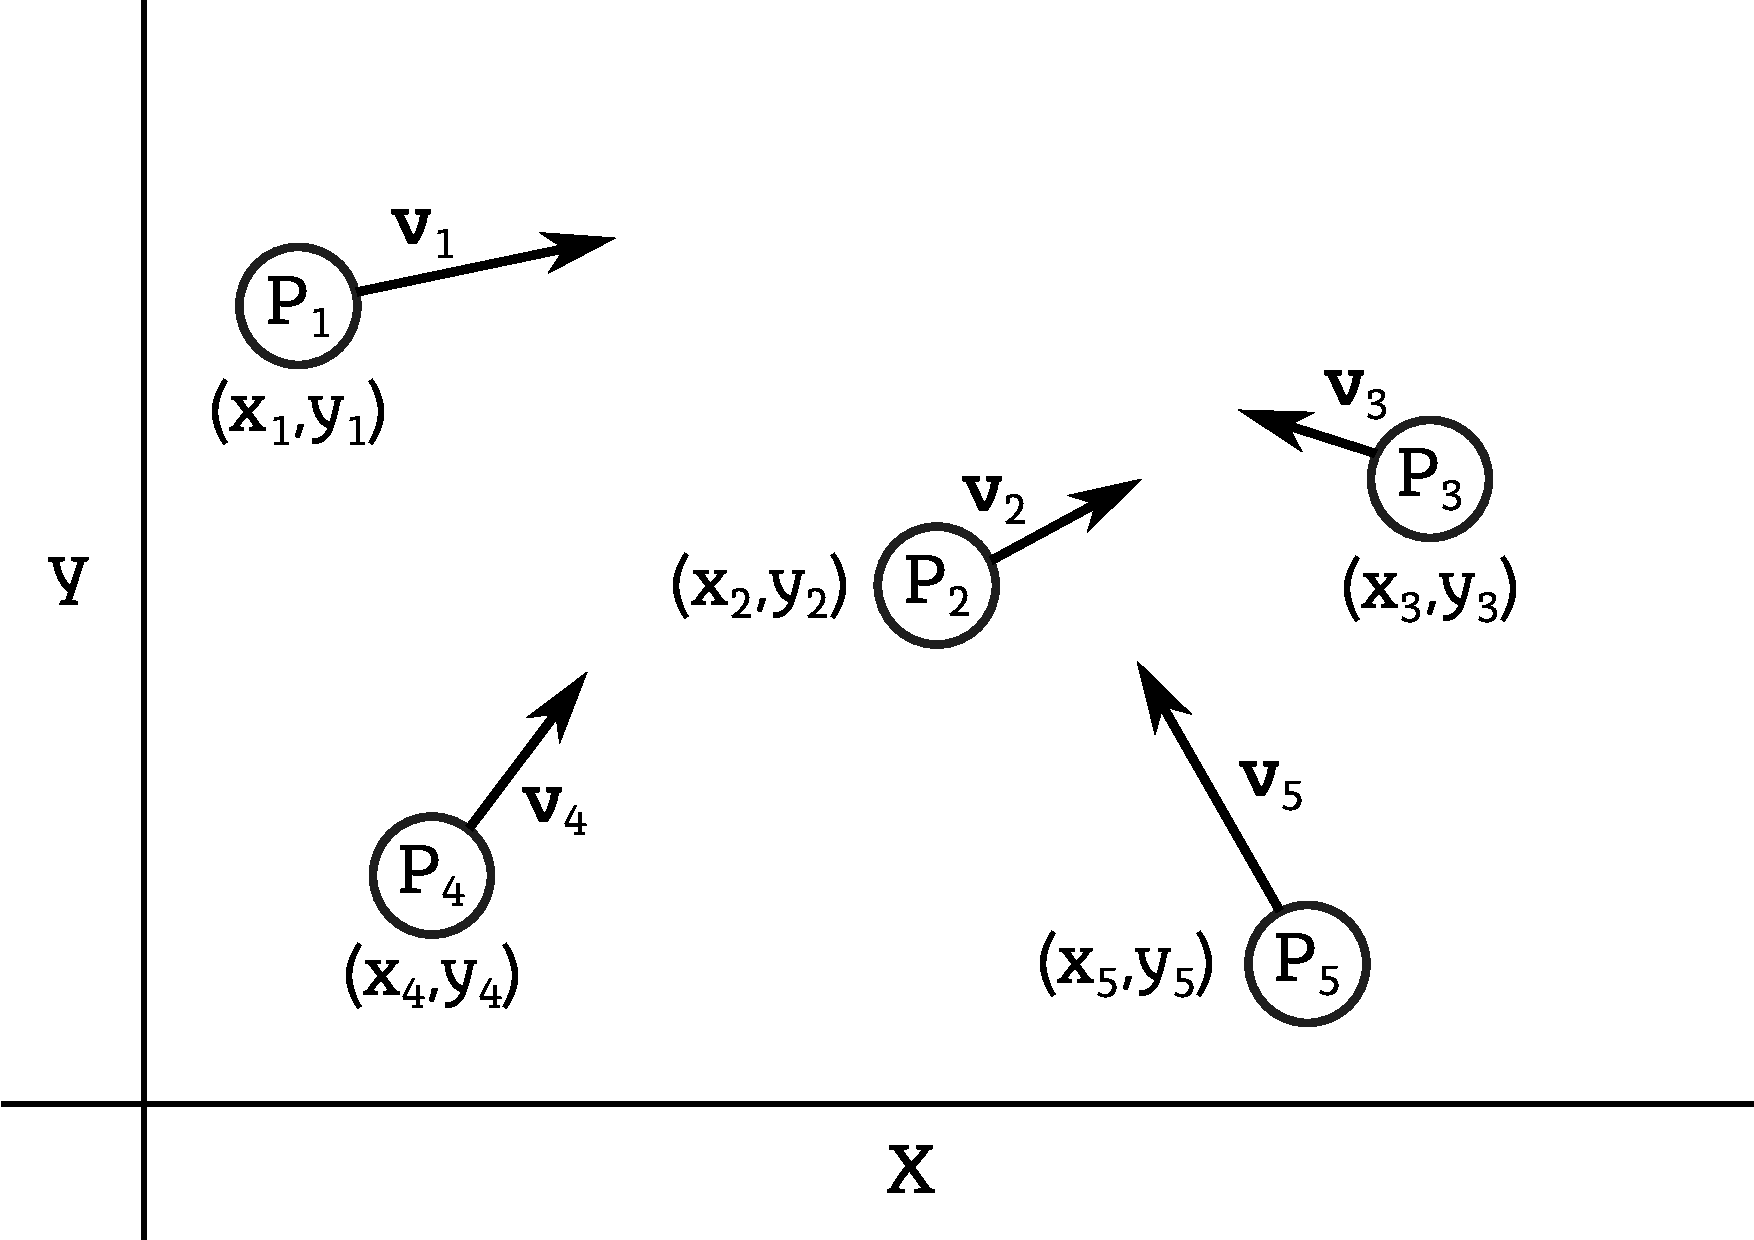
\includegraphics[width=0.6\linewidth]{./Irudiak/PSO_1}
\caption{PSO algoritmoak erabiltzen dituen partikulen adibidea. Partikula bakoitzak bere kokapena $(x_i,y_i)$ eta bere abiadura ($\mathbf{v}_i$) du}\label{fig:PSO}
\end{figure}


Animali talde hauen portaera inspiraziotzat hartuta, 1995ean Kennedy eta Eberhartek \textit{Particle Swarm Optimization} (PSO) algoritmoa proposatu zuten \cite{kennedy1995}, optimizazio numerikoko problemak ebazteko\footnote{Hau da, atal honetan ikusiko dugun algoritmoak bektore errealekin dihardu. Edonola ere, problema konbinatorialak ebazteko PSO bertsioak ere aurki daitezke.}. Algoritmoaren ideia sinplea da oso; bilaketa espazioan barrena mugitzen den partikula multzo bat erabiltzen da bilaketa aurrera eramateko. 

Uneoro partikula bakoitzak kokapen eta abiadura zehatz bat izango du, \ref{fig:PSO} irudian erakusten den bezala. Partikula bakoitzaren posizioak problemarako soluzio bat adieraziko du. Irudiko adibidean bilaketa espazioak bi aldagai besterik ez ditu ($X$ eta $Y$), eta sisteman 5 partikula daude, $P_1$, $P_2$, $P_3$, $P_4$ eta $P_5$-era.

Bilaketa gauzatzeko, PSO algoritmoaren iterazio bakoitzean partikula guztien kokapena eguneratzen da, haien abiadurak erabiliz. Partikulen abiadurak finko mantendu ezkero, denak infinitura joango lirateke. Hori ez gertatzeko, iterazio bakoitzean abiadura ere eguneratu behar da; azken eguneraketa honetan datza, hain zuzen, algoritmoaren gakoa. 

Lehen aipatu bezala, algoritmoaren inspirazioa txori-maldoen portaera da. Txori bakoitzak nora mugitu behar den erabakitzeko, bere ingurunean dauden txoriei erreparetzen die. Era berean, algoritmoan partikula baten abiadura eguneratzeko partikula horrek duen informazioa ez ezik, inguruneko partikulek dutena ere erabiltzen da. Hain zuzen ere, $i$. partikularen abiadura eguneratzeko ondoko ekuazioa erabiltzen da:

\begin{align*}
\mathbf{v}_i(t) = \mathbf{v}_i(t-1) +  C_1 \mathbf{\rho}_1 [\mathbf{p}_i - \mathbf{x}_i(t-1)] + C_2 \mathbf{\rho}_2 [\mathbf{p}_g - \mathbf{x}_i(t-1)]
\end{align*}

Ekuazio hau hiru osagaiz osatuta dago:

\begin{itemize}
\item $\mathbf{v}_i(t-1)$ - $i$. partikulak aurreko iterazioan zeukan abiadura; termino honek partikularen inertzia adirazten du.
\item $C_1 {\mathbf \rho_1} [\mathbf{p}_i - \mathbf{x}_i(t-1)]$ - Termino honetan $\mathbf{p}_i$-k $i$. partikulak bilaketa prozesuan topatu duen soluziorik onena adierazten du --ingelesez \eng{personal best} deritzona--. Termino honek eguneraketaren alderdi \hgl{kognitiboa} adierazten du, hots, partikulak berak jasotako informazioa. $C_1$ konstantea terminoaren eragina definitzeko erabiltzen da eta $\mathbf{\rho}_1$ soluzioaren tamainako ausazko bektore bat da.
\item $C_2 \mathbf{\rho}_2 [\mathbf{p}_g - \mathbf{x}_i(t-1)]$ - Termino honetan $\mathbf{p}_g$-k $i$. partikularen inguruan dauden partikulek bilaketa prozesuan topatu duten soluziorik onena adierazten du --ingelesez \eng{global best} deritzona--. Termino honek eguneraketaren alderdi \hgl{soziala} adierazten du, hots, beste partikulengandik jasotako informazioa. $C_2$ konstantea terminoaren eragina definitzeko erabiltzen da eta $\mathbf{\rho}_2$ soluzioaren tamainako ausazko bektore bat da.
\end{itemize}


Ekuazioaren azken terminoak partikulen arteko elkarrekintza simulatzen du. Horretarako, partikulen ingurune-egitura definitu behar da. Kasu honetan, ingurune kontzeptua ez da bilaketa lokalean erabiltzen den berdina, partikula bakoitzaren ingurunea aurrez ezarritakoa baita; ez du partikularen kokapenarekin zerikusirik, alegia. Partikula bakoitzaren ingurunea grafo baten bidez adieraz daiteke, non bi partikula konektatuta dauden baldin eta soilik baldin bata bestearen ingurunean badaude. 

Lehenengo hurbilketa, grafo osoa erabiltzea da, hots, edozein partikularen ingurunean beste gainontzeko partikula guztiak egongo dira; hurbilketa sofistikatuago batzuk, grafo osoa erabili beharrean, beste zenbait topologia erabiltzen dituzte (eraztunak, izarrak, toroideak, etab.).

Abiaduren eguneraketari buruzko azken puntu bezala esan beharra dago, goian dagoen ekuazioa zuzenean erabiltzen bada, abiadurak dibergitzeko joera izango duela, alegia, abiaduraren modulua gero eta handiagoa izango da. Arazo hau ekiditeko, kalkulatutako abiadurari muga bat ezartzea ohikoa izaten da.

Behin uneko iterazioaren abiadura kalkulatuta, abiadura partikularen kokapena eguneratzeko erabiltzen da:

\begin{align*}
\mathbf{x}_i(t) = \mathbf{x}_i(t-1) + \mathbf{v}_i(t-1)
\end{align*}


\begin{ifalgorithm}[t]\label{alg:pso}
\begin{ifpseudo}{PSO algoritmoa}
\item \In\ \texttt{initialize\_position}, \texttt{initialize\_velocity}, \texttt{update\_velocity}, \texttt{evaluate} eta \texttt{stop\_criterion} operadoreak
\item \In\ \texttt{num\_particles} partikula kopurua
\item \Out\ \texttt{opt\_solution}
\item \texttt{gbest = p[1]}
\item \textbf{for each} \texttt{i} \textbf{in} \texttt{1:num\_particles} \Do
\item \T{\texttt{p[i]=initialize\_position(i)}}
\item \T{\texttt{v[i]=initialize\_velocity(i)}}
\item \T{\texttt{pbest[i]=p[i]}}
\item \T{\If \texttt{evaluate(p[i])<evaluate(gbest)}}
\item \TT{\texttt{gbest = p[i]}}
\item \T{\EIf}
\item \Done
\item \While !\texttt{stop\_criterion()} \Do
\item \T{\textbf{for each} \texttt{i} \textbf{in} \texttt{particle\_set}}
\item \T{\Do}
\item \TT{\texttt{v[i]} = update\_velocity(i)}
\item \TT{\texttt{p[i] = p[i] + v[i]}}
\item \TT{\If \texttt{evaluate(p[i])<evaluate(pbest[i])}}
\item \TTT{\texttt{pbest[i]}=\texttt{p[i]}}
\item \TT{\EIf}
\item \TT{\If \texttt{evaluate(p[i])<evaluate(gbest)}}
\item \TTT{\texttt{gbest}=\texttt{p[i]}}
\item \TT{\EIf}
\item \T{\Done}
\item \Done
\item \texttt{opt\_solution = gbest}
\end{ifpseudo}
\caption{\textit{Particle Swarm Optimization} algoritmoaren sasikodea}
\end{ifalgorithm}


Iterazio bakoitzean lortutako soluzio --hots, posizio-- berriak ebaluatu eta, behar izanez gero, partikulen \eng{personal} ($\mathbf{p}_i$) eta \eng{global best} ($\mathbf{p}_g$) balioak eguneratu behar dira. Urrats guzti hauek \ref{alg:pso} algoritmoan biltzen dira.


Algoritmo hau \code{metaheuR} paketeko \code{basicPso} funtzioan inplementaturk dago. Erabilera erakusteko, optimizazio numerikoan \eng{benchmark} gisa erabiltzen den Rosenbrock funtzioa erabiliko dugu; problema sortzeko \code{rosenbrockProblem} funtzioa erabili behar dugu.


\begin{knitrout}
\definecolor{shadecolor}{rgb}{1, 1, 1}\color{fgcolor}\begin{kframe}
\begin{alltt}
\hlstd{> }\hlstd{n} \hlkwb{<-} \hlnum{10}
\hlstd{> }\hlstd{rsb.problem} \hlkwb{<-} \hlkwd{rosenbrockProblem}\hlstd{(}\hlkwc{size}\hlstd{=n)}
\end{alltt}
\end{kframe}
\end{knitrout}

Algoritmoa aplikatu ahal izateko, partikula kopurua, hasierako kokapenak eta abiadurak, abiadura maximoa, \eng{personal best} koefizientea eta \eng{global best} koefizientea ezarri behar ditugu:

\begin{knitrout}
\definecolor{shadecolor}{rgb}{1, 1, 1}\color{fgcolor}\begin{kframe}
\begin{alltt}
\hlstd{> }\hlstd{nparticles} \hlkwb{<-} \hlnum{100}
\hlstd{> }\hlstd{ipos} \hlkwb{<-} \hlkwd{lapply}\hlstd{(}\hlnum{1}\hlopt{:}\hlstd{nparticles,}
\hlstd{+ }               \hlkwc{FUN}\hlstd{=}\hlkwa{function} \hlstd{(}\hlkwc{i}\hlstd{) \{}
\hlstd{+ }                 \hlkwd{return}\hlstd{(}\hlkwd{runif}\hlstd{(n))}
\hlstd{+ }               \hlstd{\})}
\hlstd{> }\hlstd{args} \hlkwb{<-} \hlkwd{list}\hlstd{()}
\hlstd{> }\hlstd{args}\hlopt{$}\hlstd{initial.positions}  \hlkwb{<-} \hlstd{ipos}
\hlstd{> }\hlstd{args}\hlopt{$}\hlstd{initial.velocity}   \hlkwb{<-} \hlnum{0}
\hlstd{> }\hlstd{args}\hlopt{$}\hlstd{max.velocity}       \hlkwb{<-} \hlnum{5}
\hlstd{> }\hlstd{args}\hlopt{$}\hlstd{c.personal}         \hlkwb{<-} \hlnum{2}
\hlstd{> }\hlstd{args}\hlopt{$}\hlstd{c.best}             \hlkwb{<-} \hlnum{4}
\end{alltt}
\end{kframe}
\end{knitrout}

Horrez gain, helburu funtzioa eta baliabide konputazionalak ere finkatu behar ditugu.

\begin{knitrout}
\definecolor{shadecolor}{rgb}{1, 1, 1}\color{fgcolor}\begin{kframe}
\begin{alltt}
\hlstd{> }\hlstd{args}\hlopt{$}\hlstd{evaluate}  \hlkwb{<-} \hlstd{rsb.problem}\hlopt{$}\hlstd{evaluate}
\hlstd{> }\hlstd{args}\hlopt{$}\hlstd{resources} \hlkwb{<-} \hlkwd{cResource}\hlstd{(}\hlkwc{time}\hlstd{=}\hlnum{10}\hlstd{)}
\hlstd{> }
\hlstd{> }\hlstd{res.pso} \hlkwb{<-} \hlkwd{do.call}\hlstd{(basicPso, args)}
\hlstd{> }
\hlstd{> }\hlkwd{plotProgress}\hlstd{(res.pso,} \hlkwc{x}\hlstd{=}\hlstr{"iterations"}\hlstd{,} \hlkwc{y}\hlstd{=}\hlstr{"best"}\hlstd{)} \hlopt{+} \hlkwd{labs}\hlstd{(}\hlkwc{y}\hlstd{=}\hlstr{"Best Solution"}\hlstd{)}
\hlstd{> }\hlkwd{plotProgress}\hlstd{(res.pso,} \hlkwc{x}\hlstd{=}\hlstr{"iterations"}\hlstd{)} \hlopt{+} \hlkwd{labs}\hlstd{(}\hlkwc{y}\hlstd{=}\hlstr{"Average Solution"}\hlstd{)}
\end{alltt}
\end{kframe}
\end{knitrout}

\ref{fig:Rosenbrock} irudiak bilaketaren progresioa erakusten du. Ezkerreko grafikoan partikulen batazbesteko ebaluazioa erakusten da, iterazioz iterazio; eskubikoan, berriz, bilaketan zehar topatutako soluziorik onenaren \eng{fitness}-aren progresioa erakusten da. Beste algoritmoetan ez bezala, partikulen helburu funtzioen balioek ez dute konbergitzen; hala eta guztiz ere, bilaketak aurrera egiten du eta, azkenean, optimotik oso hurbil gelditzen da --Rosenbrock funtzioaren balio minimoa 0 da--.


\begin{figure}[t]
\subfigure[Batazbesteko soluzioaren progresioa]{
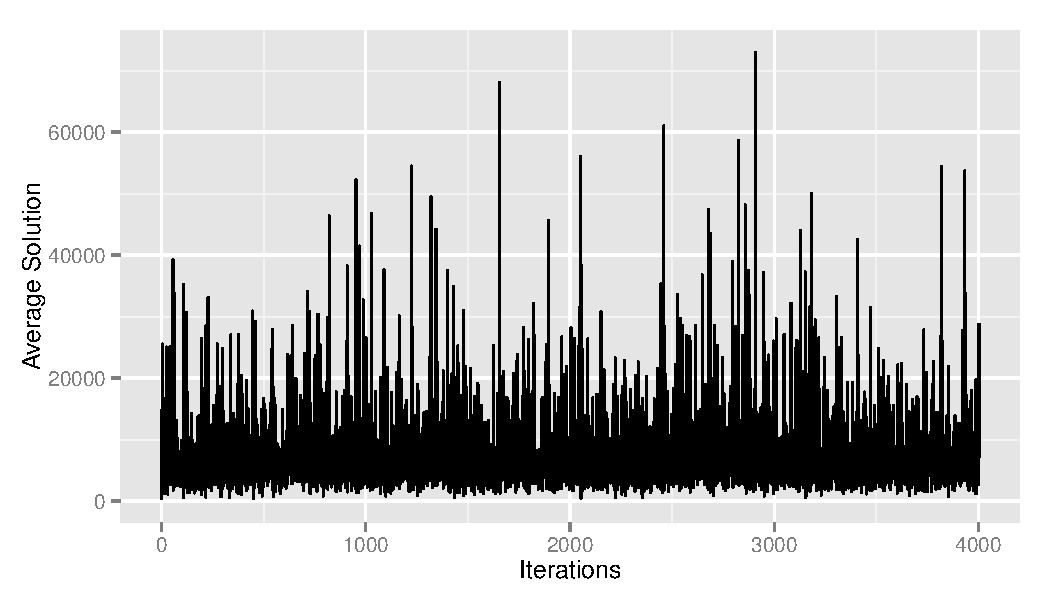
\includegraphics[width=0.45\textwidth] {./Irudiak/PSO_3-2}
}\qquad
\subfigure[Soluzio onenaren progresioa]{
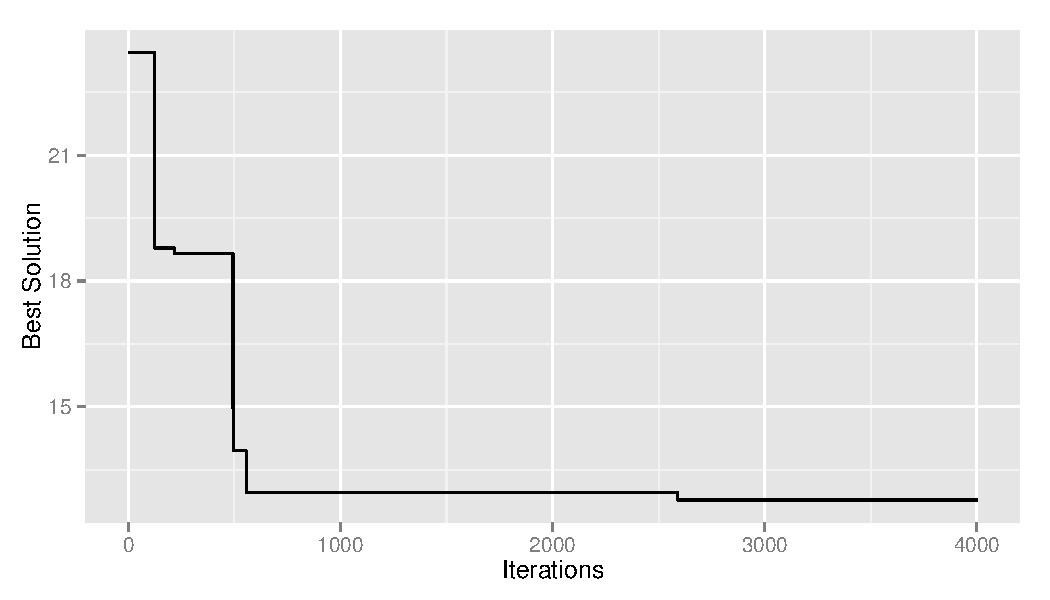
\includegraphics[width=0.45\textwidth] {./Irudiak/PSO_3-1}
}\\
\caption{PSO algoritmoaren progresioa Rosenbrock probleman}\label{fig:Rosenbrock}
\end{figure}


\bibliographystyle{plain}
\bibliography{references}

\end{document}
